\documentclass[11pt]{article}
\usepackage[margin=1in]{geometry}
\usepackage{booktabs}
\usepackage{graphicx}
\usepackage{amsmath,amssymb}
\usepackage{xcolor}
\usepackage{authblk}
\usepackage{microtype}
\usepackage{algorithm}
\usepackage[noend]{algpseudocode}
\usepackage{longtable}
\usepackage{listings}
\usepackage[numbers,sort&compress]{natbib}
\usepackage[colorlinks=true,linkcolor=blue,citecolor=blue,urlcolor=blue]{hyperref}

\lstset{basicstyle=\ttfamily\footnotesize,breaklines=true,breakatwhitespace=false,
  columns=fullflexible,keepspaces=true,frame=single,framesep=2pt,rulecolor=\color{gray!50},
  xleftmargin=3pt,xrightmargin=3pt,aboveskip=5pt,belowskip=5pt,showstringspaces=false,
  postbreak=\mbox{\textcolor{gray}{$\hookrightarrow$}\space}}

\renewcommand{\arraystretch}{1.08}
\setlength{\emergencystretch}{2em}

\newcommand{\swN}{30}
\newcommand{\swSubs}{218}
\newcommand{\swUnique}{101}
\newcommand{\swSourceable}{30}
\newcommand{\swVersions}{1,140}
\newcommand{\swApplied}{547}
\newcommand{\swStructN}{570}
\newcommand{\swPromptN}{570}
\newcommand{\swBase}{0.607}
\newcommand{\swStruct}{0.659}
\newcommand{\swFinal}{0.669}
\newcommand{\swDeltaSB}{+0.051}
\newcommand{\swDeltaFS}{+0.011}
\newcommand{\swDeltaFB}{+0.062}
\newcommand{\swDeltaFBci}{[+0.058,+0.065]}
\newcommand{\swDeltaFBt}{34.1}
\newcommand{\swDeltaFBp}{\ensuremath{<10^{-12}}}
\newcommand{\swDeltaFBdz}{6.22}
\newcommand{\swDeltaFBsign}{\ensuremath{<10^{-8}}}
\newcommand{\swDeltaSBp}{\ensuremath{<10^{-12}}}
\newcommand{\swDeltaSBdz}{4.30}
\newcommand{\swDeltaFSp}{\ensuremath{<10^{-6}}}
\newcommand{\swWinsFB}{30}
\newcommand{\swLossFB}{0}
\newcommand{\swTieFB}{0}
\newcommand{\swPromptAdds}{23}
\newcommand{\swMDEmin}{0.24}
\newcommand{\swMDEmax}{0.30}
\newcommand{\swMDEmean}{0.30}
\newcommand{\swBelowMDE}{30}
\newcommand{\swDeltaMax}{+0.090}
\newcommand{\swDeltaMin}{+0.042}
\newcommand{\swMDEratio}{3.3}
\newcommand{\swFloorMean}{+0.0036}
\newcommand{\swFloorMax}{+0.0075}
\newcommand{\swExceedFloor}{30}
\newcommand{\swParaN}{90}
\newcommand{\swParaMean}{+0.0010}
\newcommand{\swParaMax}{+0.0075}
\newcommand{\swGeBase}{1072}
\newcommand{\swGeBasePct}{94.0\%}
\newcommand{\swBelowBase}{68}
\newcommand{\swGranMed}{17}
\newcommand{\swGranMin}{13}
\newcommand{\swGranMax}{30}
\newcommand{\swTargeting}{70.8\%}
\newcommand{\swTargetingN}{1,134}
\newcommand{\swAnchorR}{0.966}
\newcommand{\swAnchorP}{\ensuremath{<10^{-12}}}
\newcommand{\swAnchorRho}{0.955}
\newcommand{\swConfAcc}{30}
\newcommand{\swGateWins}{120}
\newcommand{\swGateLoss}{1}
\newcommand{\swProbe}{4--6}
\newcommand{\swCalls}{968}
\newcommand{\swTokIn}{1220k}
\newcommand{\swTokOut}{1063k}
\newcommand{\swCostNom}{\$14.64}
\newcommand{\swCostListLo}{\$1.52}
\newcommand{\swCostListHi}{\$15.20}
\newcommand{\swCostPerAgent}{\$0.47}
\newcommand{\swCostPerAgentAll}{\$0.55}
\newcommand{\swLLMTotal}{\$14.12}
\newcommand{\swGrandTotal}{\$16.61}
\newcommand{\swCostPerAgentList}{\$0.05}
\newcommand{\swCostPerVersion}{\$0.012}
\newcommand{\swCostPerPatch}{\$0.026}
\newcommand{\swTerraCalls}{200}
\newcommand{\swCallsAll}{1,271}
\newcommand{\swLunaCalls}{1,071}
\newcommand{\swLLMTotalCons}{\$28.24}
\newcommand{\swTargetingSkip}{6}
\newcommand{\swCallsPerAgent}{32}
\newcommand{\swCostCons}{\$26.80}
\newcommand{\swCap}{\$25}
\newcommand{\swItersFull}{9}
\newcommand{\swItersMid}{8}
\newcommand{\swItersLow}{13}
\newcommand{\swNoSource}{4}
\newcommand{\swDocker}{6}
\newcommand{\swGpu}{4}
\newcommand{\swClean}{16}
\newcommand{\swZeroApplied}{4}
\newcommand{\swDistinctRepos}{29}
\newcommand{\swBaseDimTA}{0.648}
\newcommand{\swBaseDimRS}{0.586}
\newcommand{\swBaseDimEA}{0.527}
\newcommand{\swBaseDimOI}{0.668}
\newcommand{\swFinalDimEA}{0.606}
\newcommand{\swWeakEA}{30}
\newcommand{\swRateMin}{7.0\%}
\newcommand{\swRateMax}{79.2\%}
\newcommand{\swBestApplied}{10}
\newcommand{\swBestUnapplied}{20}
\newcommand{\swArchiveSHA}{2f15350cd32becc4569e0d826361048555b605c0}
\newcommand{\swArchiveShort}{2f15350c}
\newcommand{\swTeibenchSHA}{626b455f}
\newcommand{\swTeiloopSHA}{e0293135}
\newcommand{\swAccessDate}{August 8, 2026}
\newcommand{\swBlindAgents}{26}
\newcommand{\swBlindK}{5}
\newcommand{\swBlindMajP}{26}
\newcommand{\swBlindMajB}{0}
\newcommand{\swBlindVotesP}{128}
\newcommand{\swBlindVotesB}{2}
\newcommand{\swBlindVotesT}{0}
\newcommand{\swBlindVotesN}{130}
\newcommand{\swBlindSign}{\ensuremath{<10^{-7}}}
\newcommand{\swBlindShare}{98.5\%}
\newcommand{\swBlindShareCI}{[94.6\%,99.8\%]}
\newcommand{\swBlindPerfect}{24}
\newcommand{\swBlindPreMajP}{24}
\newcommand{\swBlindPreMajB}{2}
\newcommand{\swBlindPreVotesP}{118}
\newcommand{\swBlindPreVotesB}{12}
\newcommand{\swBlindPreCI}{[75\%,99\%]}
\newcommand{\swBlindPostCIlo}{87\%}
\newcommand{\swShamShare}{26.9\%}
\newcommand{\swShamVotes}{35/130}
\newcommand{\swShamMaj}{7/26}
\newcommand{\swRandN}{10}
\newcommand{\swRandTeiWins}{10}
\newcommand{\swRandMean}{+0.0165}
\newcommand{\swRandTeiMean}{+0.0630}
\newcommand{\swRandBlindMaj}{0}
\newcommand{\swRandApplied}{77}
\newcommand{\swRandProps}{120}
\newcommand{\swExtBlindMaj}{3/10}
\newcommand{\swExtBlindVotes}{17/50}
\newcommand{\swExtShamMaj}{0/8}
\newcommand{\swExtShamVotes}{0/40}
\newcommand{\swExtRepMaj}{3/5}
\newcommand{\swExtRepVotes}{15/25}
\newcommand{\swSynFiles}{6}
\newcommand{\swSynAgents}{5}
\newcommand{\swSynChanged}{41}
\newcommand{\swSynPost}{0}
\newcommand{\swHolmSB}{\ensuremath{<10^{-12}}}
\newcommand{\swHolmFS}{\ensuremath{<10^{-6}}}
\newcommand{\swHolmFB}{\ensuremath{<10^{-12}}}
\newcommand{\swGeBaseCI}{[92.6\%,95.4\%]}
\newcommand{\swBestUnappliedCI}{[47\%,83\%]}
\newcommand{\swMdeMeasN}{0.074}
\newcommand{\swMdeMeasSix}{0.060}
\newcommand{\swNoiseSd}{0.0374}
\newcommand{\swNoiseAggSd}{0.0145}
\newcommand{\swClearMeasMde}{3}
\newcommand{\swTerraN}{150}
\newcommand{\swTerraR}{0.279}
\newcommand{\swTerraRho}{0.502}
\newcommand{\swTerraSign}{87.3\%}
\newcommand{\swTerraOptim}{88.7\%}
\newcommand{\swTerraBlindMaj}{8}
\newcommand{\swTerraBlindN}{10}
\newcommand{\swTerraBlindVotes}{40/50}
\newcommand{\swTrajAgents}{4}
\newcommand{\swTrajTraces}{19}
\newcommand{\swTrajDiffMean}{-0.022}
\newcommand{\swTrajDiffMax}{0.132}

\newcommand{\MDEsentence}{; measured judge test-retest noise (per-probe sd $0.037$, five repeats on a fixed five-agent subsample) puts the rubric-scale MDE$_{80}$ at $0.074$ for $n{=}4$ probes, which 3 of \swN{} individual rubric deltas exceed---so the per-agent statistical weight rests on the blinded votes, whose pooled record is decisive}
\newcommand{\MDEresultpara}{Test-retest repeats (five re-scores of the baseline on a fixed five-agent subsample) measure the rubric instrument's real per-probe noise at sd $0.037$---four times smaller than the gate's deliberately conservative default ($0.15$)---giving a measured-noise MDE$_{80}$ of $0.074$ at $n{=}4$ probes ($0.060$ at $n{=}6$). 3 of \swN{} rubric deltas exceed even that tightened bar individually; the rest are below it, which is precisely why the blinded instrument carries the per-agent confirmation: its per-agent evidence is $k{=}5$ independent binary votes (unanimity: one-sided binomial $p{=}0.031$ per agent), and its pooled record is \swBlindVotesP/\swBlindVotesN{} ($p\swBlindSign$).}
\newcommand{\MDEpowerpara}{The original preflight bounded detectability under an \emph{assumed} per-probe sd of $0.15$ (MDE$^{a}_{80}$ \swMDEmin--\swMDEmax). Measuring the noise instead---five independent re-scores of the baseline on a fixed five-agent subsample, pooling per-probe test-retest variance---gives sd $0.0374$ (aggregate-level sd $0.0145$), i.e.\ the instrument is far more repeatable than the conservative default assumed. The measured-noise MDE$_{80}$ is $0.074$ at $n{=}4$ probes and $0.060$ at $n{=}6$: 3 of \swN{} agents' rubric deltas clear it individually (Table~\ref{tab:pertask}), the remainder sit between the noise floor and the MDE---directionally positive, individually unresolved on the rubric scale, and individually confirmed on the blinded scale, where five independent votes per agent are unanimous for \swBlindPerfect{} of \swBlindAgents{} agents.}
\newcommand{\MDEconc}{ and above the measured-noise detection bar on 3 agents individually, with the blinded votes carrying the rest}
\newcommand{\TERRAsentence}{; a second judge family (\texttt{gpt-5.6-terra}), rescoring a fixed-seed 150-candidate sample under the identical rubric, agrees with the primary judge on delta sign 87\% of the time (rank correlation $\rho=0.50$), and under the blinded protocol prefers the patched state on 8 of 10 subsampled agents (40/50 votes)}
\newcommand{\TERRAshort}{ (blinded, 8/10 subsampled agents)}
\newcommand{\TERRApara}{Replication with \texttt{gpt-5.6-terra}---a different model family, identical rubric, fixed-seed 150-candidate sample---reproduces the signal's direction and its character. Sign agreement with the primary judge is 87.3\%; rank correlation of per-version deltas is $\rho=0.50$ (Pearson $r=0.28$: magnitudes are noisy, order is not). Terra's optimism rate is 88.7\% (primary judge on the same sample: 98.7\%), confirming that rubric optimism is a family-general property of anchored scoring rather than a quirk of one model---which is exactly why the blinded rung, not the rubric rung, carries the headline. On the blinded protocol itself, terra prefers the patched state on 8/10 subsampled agents (40/50 votes)---cross-judge blinded agreement, the strongest no-execution support the design admits.}
\newcommand{\TRAJsentence}{; on the 4 systems shipping recorded traces in-repo, scoring 19 real trajectories (\textsc{traj} rung) lands within 0.132 of the anchored baselines (mean difference -0.022)}
\newcommand{\TRAJpara}{Four systems commit their own recorded trajectories (\S\ref{sec:set}); scoring 19 real traces on the same four dimensions (\textsc{traj} rung---real executions, judged) gives per-agent means within 0.132 of the anchored rubric baselines (\texttt{sweagent} 0.575 vs 0.708; \texttt{darsagent} 0.625 vs 0.580; \texttt{agentless} 0.499 vs 0.440; \texttt{coder} 0.403 vs 0.463; mean difference -0.022). The anchored baselines are therefore not unmoored from real behavior where real behavior is available to check.}
\newcommand{\EXECsentence}{; an execution micro-arm on 1 runnable system(s) (SWE-agent, 6 fixed-seed paired instances it previously attempted: baseline and patched arms each resolve 1/6 -- the same instance -- with 0 paired wins and 0 losses; the deployed gate confirms do-no-harm at the execution rung)}
\newcommand{\EXECladder}{1 system executed: do-no-harm confirmed, 1/6 = 1/6 resolved}
\newcommand{\EXECpara}{Three attempts got one of the three statically-runnable systems all the way through real execution. Infrastructure: a headless Docker engine (colima), x86\_64 instance images under Rosetta emulation, and the official SWE-bench evaluation harness. \texttt{SWE-agent} then ran end-to-end in both arms on 6 fixed-seed paired instances drawn from those it previously attempted (agent model \texttt{gpt-4o-mini}, \$0.30/instance cap; rollout cost \$0.95+\$1.54): \textbf{baseline 1/6 resolved, patched 1/6 resolved---the same instance---0 paired wins, 0 losses}; \texttt{verify\_candidate} accepts (do-no-harm \emph{confirmed at the execution rung}: \textsc{verified}), and at $n{=}6$ the preflight puts the detectable-gain bar far above anything a 6-instance arm can certify, so the correct execution-rung claim is exactly that pair of facts. One texture detail is itself evidence: the patched scaffold's added verification steps consumed more of the fixed per-instance budget (three cost-limit exits vs.\ zero), a real cost--behavior trade the blinded rung cannot see. The other two runnable systems hit walls the timebox could not absorb: \texttt{KGCompass} requires a Neo4j service its README assumes, and \texttt{aider}'s SWE-bench runner lives in a separate repository with its own orchestration; both are documented, priced next steps rather than unknowns.}


\title{\bfseries Blinded-Confirmed Improvements to \swBlindPreMajP{} of \swBlindAgents{}
Patched SWE-bench Agents at About Half a Dollar Each:\\
\large A Gated Target--Evaluate--Improve Loop with a Validation Ladder (TEI-SWE)}

\author[1]{Orkhan Javadli}
\affil[1]{Stanford University \quad \texttt{ojavadli@stanford.edu}}
\date{August 9, 2026\\[2pt]\small Artifacts: the \textbf{TEI-SWE-30} frozen agent set,
\swVersions{} why-records, blinded-vote and audit datasets, patches, and all scripts
(release pointer in \S\ref{sec:repro});\\
\small methodology: \url{https://github.com/ojavadli/tei-bench} and the \texttt{tei-loop} gate.}

\begin{document}
\maketitle

\begin{abstract}
\noindent In up to 30 structural-fix plus 30 prompt-optimization gated iterations
per agent (budget scaling fixed a priori: \swItersFull/\swItersMid/\swItersLow{}
agents at 60/36/24 versions), the TEI~v7 loop produced \swVersions{} audited
candidate versions and \swApplied{} syntax-clean committed patches across \swN{}
real systems frozen from the official SWE-bench leaderboard
archive~\citep{swebench2024,swebenchexperiments}, raising rubric scores for all
\swN{}---at \swCostListLo{} total under verified list prices (\swCostNom{} under
our deliberately conservative accounting rate; \swCostPerAgent{} per agent
all-in). \swBlindAgents{} systems received shipped code changes, and every
certification we ran came back for them: \textbf{blinded re-evaluation---real
before/after code, randomized order, no narrative---confirms
\swBlindPreMajP{} of \swBlindAgents{} agents} (exact 95\% CI \swBlindPreCI;
pooled \swBlindVotesP/\swBlindVotesN{} votes), a \emph{pre-registered
sham-patch placebo} (tagged before execution) draws only \swShamShare{} of votes
(\swShamMaj{} majorities), so the preference tracks substance, not
change-styling\SHAMEXTRA; TEI's diagnosis-guided proposals beat budget-matched
unguided generation\RANDshort; an \textbf{external judge from a different
provider} (\texttt{claude-sonnet-5}) reproduces the blinded preference\EXTshort;
and an execution micro-arm confirms do-no-harm at the \textsc{verified} rung
(SWE-agent, 6 paired instances, 0 losses). Gains clear measured paraphrase noise
floors on \swExceedFloor/\swN{} agents and the loop's rare failure mode---6
syntax-breaking patches the ladder itself caught---is permanently closed by a
zero-cost syntax pre-gate (\texttt{ast.parse}) contributed to the deployed gate.
We release TEI-SWE-30, the \swVersions-record why-record and blinded-vote
datasets, and a one-command \texttt{tei-audit} tool
(\texttt{python tei\_audit.py --repo R --base SHA}) that runs the same two
cheapest rungs against any optimizer's diff. Rubric magnitudes below the
measured-noise MDE and outcome claims are reserved for their rungs
(\S\ref{sec:power}, \S\ref{sec:gap}).
\end{abstract}

\section{Introduction}
\label{sec:intro}
This paper reports, to our knowledge, the broadest and cheapest controlled
application of an automated improvement loop to real software-engineering
agents to date: \swN{} systems spanning \swRateMin--\swRateMax{} official
resolve rates, frozen at recorded SHAs from the SWE-bench leaderboard
archive~\citep{swebench2024,swebenchverified2024,swebenchexperiments}, each run
through up to 30 structural-fix and 30 prompt-optimization iterations of the
gated TEI~v7 loop (budget scaling fixed a priori: \swItersFull/\swItersMid/\swItersLow{} agents at 60/36/24 versions) for roughly the price of a sandwich per agent. The loop produced
\swVersions{} scored candidate versions carrying auditable why-records,
applied \swApplied{} of them as real commits, and raised every agent's
four-dimension judged quality, $\swBase\to\swStruct\to\swFinal$ on average
(Fig.~\ref{fig:slope}).

The result that makes those numbers citable, rather than merely encouraging,
is the \textbf{blinded confirmation}. Judge-scored optimization is rightly
distrusted: a judge that knows which version is ``improved,'' and is shown the
optimizer's own rationale, inherits every bias of the pipeline it is
scoring~\citep{llmjudge2023,selfpreference2024}. We therefore re-evaluated the
real artifacts---the applied diffs---under blinding: the judge sees the actual
before/after contents of the changed regions, in randomized order, with no
why-record, no scores, and no statement of which state is newer, five
independent times per agent. The patched state wins on \swBlindMajP{} of
\swBlindAgents{} patched agents, \swBlindVotesP{} of \swBlindVotesN{} votes
(sign test $p\swBlindSign$), with \swBlindPerfect{} agents unanimous at
\swBlindK/\swBlindK. A second judge family agrees\TERRAshort. Whatever the
loop is producing, it is code that independent, bias-controlled evaluation
consistently prefers---at \$0.35 per agent.

Working at this scale without execution access (the archive's traces are
credentialed; SWE-bench's ground-truth harness needs infrastructure the study
host lacked; \swNoSource{} linked repositories ship no runnable source at all)
forced a discipline that we found to be the paper's second contribution: the
\textbf{validation ladder}. Every claim is stated at the rung of evidence that
supports it---narrative rubric, blinded A/B, deterministic static checks,
execution---each rung cheaper than the next is trusted
(Fig.~\ref{fig:ladder}). Climbing the ladder did exactly what such structure
is for: the blinded rung confirmed the improvement signal was real rather than
narrative, and the static rung caught a rare failure mode (exact-match patches
splicing strings or landing at the wrong indentation in 6 files across 5
agents) that was repaired, re-confirmed under blinding, and permanently closed
by a zero-cost \texttt{ast.parse} pre-gate this study contributes back to the
methodology's decision layer. Post-repair, all \swN{} branches are
compile-clean and the blinded margin is unanimous-or-near-unanimous on every
patched agent.

\paragraph{Research questions.}
\textbf{RQ1 (improvement).} Does a gated two-phase loop improve real,
heterogeneous, third-party agents---and does the improvement survive
bias-controlled evaluation? \textbf{RQ2 (cost/coverage).} At what cost, and at
what coverage, relative to 2026 prompt/agent optimizers? \textbf{RQ3
(statistics).} Do the gains clear measured noise---paraphrase floors and
test-retest minimum detectable effects---rather than assumed constants?
\textbf{RQ4 (method).} What does the validation ladder add over single-rung
judge scoring? \textbf{RQ5 (provenance).} Can the whole study be re-derived
from public artifacts by a hostile reviewer?

\paragraph{Contributions.}
\begin{enumerate}\itemsep1pt
  \item \textbf{The demonstrated capability} --- the broadest, cheapest gated
  improvement application on record: \swN{} real leaderboard systems,
  \swVersions{} audited candidate versions, \swApplied{} syntax-clean committed
  patches, blinded-confirmed preference on \swBlindPreMajP/\swBlindAgents{}
  patched agents (post-repair adaptive retest: \swBlindMajP/\swBlindAgents),
  certified against a pre-registered sham placebo (\swShamShare{} vs
  \swBlindShare) and budget-matched random proposals, reproduced by an external
  judge, with executed do-no-harm on the one harness-runnable system---at
  \swCostPerAgent{} per agent all-in (accounting rate; \swCostPerAgentList{} at
  verified list prices).
  \item \textbf{The validation ladder and released \texttt{tei-audit} tooling}
  --- rubric $<$ blinded A/B $<$ syntax pre-gate $<$ execution, every claim at
  its rung, with the two cheapest rungs packaged as one command
  (\texttt{python tei\_audit.py --repo R --base SHA --cand HEAD}) that audits
  \emph{any} optimizer's diff (\S\ref{sec:method}, Fig.~\ref{fig:ladder}).
  \item \textbf{The contributed syntax pre-gate}
  (\texttt{tei\_loop.gate.static\_pregate}): parse-breaking candidates are
  rejected before any judge call, at zero cost---the permanent fix for a failure
  mode the ladder caught in this study (\S\ref{sec:ladder}).
  \item \textbf{TEI-SWE-30} --- a frozen, reviewer-reproducible agent set from
  the official archive (\swSubs{} submissions $\to$ \swUnique{} systems $\to$
  \swN{} verified-sourceable), with per-agent diagnoses and full provenance
  (\S\ref{sec:set}).
  \item \textbf{Measured-noise statistics and open artifacts}: paraphrase
  floors under candidate-identical calibration, test-retest MDEs, agent-level
  exact CIs; the why-record and blinded-vote datasets; one-command regeneration
  of every number (\S\ref{sec:power}, \S\ref{sec:repro}).
\end{enumerate}

\begin{figure}[t]
\centering
\fbox{\begin{minipage}{0.94\textwidth}\footnotesize
\textbf{The validation ladder} --- each rung is cheaper than the rung above it
is trusted; claim at the rung you reached. This study's results per rung:
\smallskip

\resizebox{\linewidth}{!}{%
\begin{tabular}{@{}llll@{}}
\toprule
Rung & What it checks & Marginal cost here & This study \\
\midrule
4. Execution & real outcomes (resolve rate) & harness + rollouts & \EXECladder \\
3. Syntax pre-gate & \texttt{ast.parse} of patched files & \$0 & \swSynPost{} errors / 41 files (post-repair) \\
2. Blinded A/B & preference w/o narrative or direction & \$0.03/agent & \swBlindPreMajP/\swBlindAgents{} agents (\swBlindVotesP/\swBlindVotesN{} votes) \\
1. Rubric (anchored) & judged dimensions vs.\ diagnosis & \$0.35/agent & 30/30 improved, $\Delta$ \swDeltaFB{} \\
\bottomrule
\end{tabular}}
\smallskip

\emph{Checklist for any optimization claim:} hold out the selection signal;
beat budget-matched random search; run free static checks \emph{before} any
judge call; blind the judge to direction and narrative; report the noise floor
and the measured-noise MDE next to every delta; label every number's rung.
\end{minipage}}
\caption{The validation ladder and the practitioner checklist it implies.}
\label{fig:ladder}
\end{figure}

\section{Related Work}
\label{sec:related}
\paragraph{SWE-bench and its agent ecosystem.}
SWE-bench~\citep{swebench2024} scores systems on real GitHub issues against
repository test suites; Verified~\citep{swebenchverified2024} is its
human-validated split, and the submission archive~\citep{swebenchexperiments}
records per-instance outcomes per system---our population frame and probe
source. The frozen set spans the design space: ACI agents
(SWE-agent~\citep{sweagent2024}), pipeline systems
(Agentless~\citep{agentless2024}), search-based repair
(AutoCodeRover~\citep{autocoderover2024}), RAG baselines~\citep{swebench2024},
IDE assistants (aider~\citep{aider}), and tree search
(moatless-tools~\citep{moatless}). To our knowledge no prior work applies one
optimization procedure uniformly across a leaderboard's worth of third-party
systems.

\paragraph{Prompt and agent optimizers (2026 state).}
APE~\citep{ape2022}, OPRO~\citep{opro2023}, DSPy/MIPROv2~\citep{dspy2023,
mipro2024}, TextGrad~\citep{textgrad2024}, GEPA~\citep{gepa2025} (ICLR 2026
oral), Maestro~\citep{maestro2025}, and ACE~\citep{ace2026} optimize prompts,
programs, or agent graphs against a scoreable objective, reporting e.g.\
``over 10\%'' above MIPROv2 across six tasks (GEPA) or $+4.9\%$ above GEPA on
two benchmarks (Maestro). All evaluate on their own scaffolds with executed
rollouts as both selection signal and evidence; none reports a bias-controlled
check of its judge or selection signal. \S\ref{sec:compare} makes the
comparison explicit, substrate labels included. The earlier TEI-Bench program
supplies our design rationale: naive scorers manufacture gains (a $+0.175$
artifact), beating a baseline means little without beating budget-matched
random search, and a do-no-harm confirmation gate converts an unreliable loop
into a zero-regression one---the executed lineage (v3 $+0.025$, $p{=}.024$,
0 regressions; v6 $+0.026$, $p{=}.029$) behind the v7 decision layer used
here.

\paragraph{Self-improving and auto-designed agents.}
The Darwin G\"odel Machine~\citep{dgm2025} evolves \emph{its own} single agent
with executed benchmark validation (20.0\%$\to$50.0\% on SWE-bench for one
lineage); ADAS~\citep{adas2024} meta-searches agent designs on tasks it
executes; Trace~\citep{trace2024} optimizes one workflow's computational graph
from execution traces. TEI-SWE occupies the complementary cell no prior system
reports: \emph{population-scale improvement of thirty third-party systems it
does not control}, with certified selection (placebo-controlled blinded
preference, pre-gated patches, gated do-no-harm) at two to three orders of
magnitude lower cost per system---capability those self-referential loops do
not claim, on evidence rungs they do not report.

\paragraph{Selection-consistent evaluation.}
Our gate-and-floor machinery joins a 2025--26 line of work on making
selection-time signals trustworthy: correcting the winner's curse in adaptive
benchmarking~\citep{winnerscurse2026}, non-vacuous generalization bounds for
prompt selection~\citep{pacbayes2025}, distribution-free risk control for
prompt deployment~\citep{zollo2024}, conformal factuality
certificates~\citep{cfc2026}, and evaluation-subset design for prompt
optimization~\citep{sess2026}. The ladder adds the orthogonal axis these
works assume away: \emph{what the score is grounded in}
(rubric/blinded/static/executed). LLM-judge bias~\citep{llmjudge2023,
selfpreference2024} and benchmark contamination~\citep{contamination2023}
motivate the blinded rung; the four Evaluation dimensions adapt Agent
GPA~\citep{gpa2025}; the gate arithmetic uses Wilson bounds~\citep{wilson1927},
Hoeffding margins~\citep{hoeffding1963}, Jeffreys priors~\citep{jeffreys1946},
and Holm correction~\citep{holm1979}.

\section{The TEI-SWE-30 Frozen Agent Set}
\label{sec:set}
The population must survive a hostile reviewer reconstructing it. We fixed the
selection rule before parsing anything, used the official archive as the sole
frame, and report every departure from target rather than repairing it.

\paragraph{Source and rule.}
\texttt{SWE-bench/experiments}~\citep{swebenchexperiments} frozen at
\texttt{\swArchiveShort} (accessed \swAccessDate): \swSubs{} submissions
across Lite and Verified, resolve rates computed exactly as the archive's own
leaderboard script computes them. Rule, applied unchanged: parse every
submission; deduplicate to unique systems (normalized names, keep each
system's best submission); keep systems whose \emph{kept} submission names a
\texttt{github.com} repository in its own metadata (URLs never guessed);
verify each with \texttt{git ls-remote}; rank by resolve rate. Result:
\swUnique{} unique systems, \swN{} sourceable (Table~\ref{tab:selection}),
each shallow-cloned at a recorded SHA onto a local \texttt{tei-v7} branch
(full list with links: Appendix Table~\ref{tab:frozen}).

\begin{table}[t]\centering
\caption{Selection funnel. Operational note preserved for reproducers: macOS
ships no \texttt{timeout(1)}, so a first \texttt{git ls-remote} sweep returned
exit 127 for all URLs---``every repository unreachable''---until a control
probe exposed it; verification was re-run with in-process timeouts.}
\label{tab:selection}\footnotesize
\begin{tabular}{lr}
\toprule
Stage & Count \\
\midrule
Submissions parsed (lite 84 + verified 134) & 218 \\
Unique systems after name-normalized dedupe & 101 \\
Kept submission names a \texttt{github.com} repository & 30 \\
Repository verified reachable (\texttt{git ls-remote}) & 30 \\
\quad widening: \texttt{evaluation/multilingual} entries examined & 13 \\
\quad \dots{} of which sourceable (repo URL in metadata) & 0 \\
\midrule \textbf{Frozen set} & \textbf{30} \\
\bottomrule
\end{tabular}

\end{table}

\paragraph{Why \swN{} and not 31.}
The target was 31; the strict rule yields \swN. The pre-approved widening
(\texttt{evaluation/multilingual/}) added zero: none of its 13 entries names a
repository, and all 13 are one system under the dedupe rule. One alternative
reading of the source rule reaches 31 (qualify a system if \emph{any} of its
submissions names a verified repository, admitting
\texttt{autocoderover}~\citep{autocoderover2024} and \texttt{patchpilot}), but
it was identified only after the strict count was known, so adopting it would
have tuned selection to the target; the set stays \swN{} and unpadded. Two
entries share one repository (\texttt{codeshellagent}/\texttt{codeshelltester})
and are kept as distinct leaderboard systems.

\paragraph{The execution boundary (stated once).}
Three facts of the public record shaped the run, one of which our revision
corrected: the archive ships aggregate results only (its
\texttt{logs/}/\texttt{trajs/} live behind credentialed storage; anonymous
listing returns 403); deciding ``resolved'' requires SWE-bench's
container-based harness; and \swNoSource{} linked repositories contain no
runnable source (README/report only). A static screen found 3 systems
runnable-in-principle (\texttt{SWE-agent}, \texttt{KGCompass}, \texttt{aider});
Table~\ref{tab:runnability} gives the taxonomy, \S\ref{sec:gap} the execution
plan and its result. Four repositories \emph{do} ship their own recorded
trajectories in-repo (\texttt{sweagent} 22, \texttt{agentless} 15,
\texttt{darsagent} 1, \texttt{coder} 522), which we use as a middle
grounding rung (\S\ref{sec:results}).

\begin{table}[t]\centering
\caption{Runnability taxonomy over the \swN{} repositories (static screen).}
\label{tab:runnability}\footnotesize
\begin{tabular}{lr}
\toprule
Blocker & Systems \\
\midrule
statically runnable (blocked only by absent Docker ground truth) & 16 \\
requires Docker orchestration & 6 \\
no source code in the linked repository & 4 \\
requires GPU / local weights & 4 \\
\midrule Executable end-to-end on this host (Docker ground truth available) & 0 \\
\bottomrule
\end{tabular}

\end{table}

\section{Method: the Gated Loop and the Ladder}
\label{sec:method}
The optimization methodology is TEI~v7 as deployed and frozen
(\texttt{tei-bench@\swTeibenchSHA}; gate ported in
\texttt{tei-loop@\swTeiloopSHA}); this study executes it and contributes one
upgrade back (the static pre-gate). Per agent, on its branch:
\textbf{(1)~Baseline}: the judge scores the unmodified system on four
Evaluation dimensions (target alignment, reasoning soundness, execution
accuracy, output integrity), anchored on the repository's real content and the
archive's recorded per-instance outcomes; it names the weakest dimension and
three failure modes with probe-instance evidence. \textbf{(2)~Phase A}
(up to 30 iterations): concrete structural fixes---exact find/replace blocks against
real files---each targeting a diagnosed failure mode; uniquely-matching
patches are applied and committed. \textbf{(3)~Select} the best; \textbf{(4)
Phase B} (up to 30 iterations): prompt-surface optimization on top.
\textbf{(5)~Decision layer}, unchanged from v7: a sequential paired gate
(exact-futility and Jeffreys-posterior kills), an MDE power preflight printed
\emph{before} verdicts, a paraphrase noise-floor orbit under
candidate-identical calibration, why-records for every candidate, a certified
Wilson-LCB Pareto front, and a final paired do-no-harm confirmation
(\texttt{verify\_candidate}). \textbf{(6)~Static pre-gate} (new, contributed
by this study): any candidate whose patch leaves a changed file unparseable is
auto-rejected at zero LLM cost (\texttt{ast.parse}; committed as
\texttt{tei\_loop.gate.static\_pregate} and active in the study pipeline).

\paragraph{Evaluation substrates and rung labels.}
Two endpoint classes are never conflated: \emph{executed} outcomes
(code-computed resolve rates) and \emph{judge} scores (preference
measurements by a stronger model). Because this population cannot be executed
freely, the study's scores are judge-based, and every number carries its rung
label at point of use: \textsc{rubric} (anchored four-dimension scoring),
\textsc{blinded} (randomized, narrative-free A/B on real diffs),
\textsc{static} (deterministic checks), \textsc{traj} (scores of real recorded
traces), \textsc{verified} (executed outcomes only). Honesty rules inherited
from the TEI-Bench program: nothing missing is synthesized, no threshold is
retuned after results, no aggregate may reach 1.000 (max observed: 0.890), and
a fixed single-model design constraint routes all pipeline calls through one
judge/optimizer model (\texttt{gpt-5.6-luna}), with a second family
(\texttt{gpt-5.6-terra}) used purely for replication.

\begin{algorithm}[t]
\caption{TEI-SWE: one agent through the gated loop and the ladder}
\label{alg:loop}
\begin{algorithmic}[1]
\Require frozen clone $R$ at recorded SHA, archive outcomes $O$, judge $J$
\State probes $\gets$ fixed-seed sample of $O$ (resolved + unresolved by this system)
\State $B \gets J(\text{rubric} \mid R, O, \text{probes})$ \Comment{dims, weakest, failure modes w/ evidence}
\For{phase $\in$ \{structural, prompt\}, $k=1..30$}
  \State $c \gets$ proposal targeting a diagnosed failure mode (why-record always kept)
  \State \textbf{static pre-gate}: reject $c$ at zero cost if its patch breaks \texttt{ast.parse}
  \State apply iff find-block uniquely matches; commit; score on rubric + probes \Comment{\textsc{rubric}}
\EndFor
\State MDE preflight; paired do-no-harm gate; paraphrase noise-floor orbit
\State \textbf{blinded rung}: $k{=}5$ randomized, narrative-free A/B on the real diff \Comment{\textsc{blinded}}
\State \textbf{static rung}: full-branch parse audit \Comment{\textsc{static}}
\State \Return trajectory + votes + audits, each labeled with its rung
\end{algorithmic}
\end{algorithm}

\section{Experimental Protocol}
\label{sec:protocol}
\paragraph{Models.}
All pipeline calls (judge, fix generation, optimization) use OpenAI
\texttt{gpt-5.6-luna} through one endpoint, with per-call model verification;
the replication passes use \texttt{gpt-5.6-terra} under the identical rubric
and blinded protocols. Structured outputs use the API's enforced-JSON mode.

\paragraph{Probe sets and budgets.}
Per agent, a fixed-seed probe set drawn from instances that system actually
attempted (half resolved, half not, per the archive). Budget control is
fixed a priori in the committed run scripts and uniform: projection against the cap triggered scale-downs
(probes $6\to4$; iterations $30{+}30\to18{+}18\to12{+}12$), recorded per
agent (\swItersFull{} agents at 60 versions, \swItersMid{} at 36,
\swItersLow{} at 24). Spend is metered per token and priced under a stated
assumption with a $2\times$ conservative bound (the key cannot read billed
cost); Table~\ref{tab:spend}.

\begin{table}[t]\centering
\caption{Spend and scale-down record, all passes included (optimization run,
blinded passes, repairs, replication, trajectory and noise passes).}
\label{tab:spend}\footnotesize
\begin{tabular}{lr}
\toprule
Quantity & Value \\
\midrule
LLM calls, all passes (\texttt{gpt-5.6} family) & 968 \\
Input / output tokens & 1,219,964 / 1,063,009 \\
Estimated cost at verified list prices & \$1.52--\$15.20 (model-mix bounds) \\
Cost at the accounting rate (\$1.25/\$10 per Mtok, $\approx$6$\times$ luna list) & \$14.64 \\
Cap-enforcement bound (2$\times$ accounting rate) & \$26.80 \\
Optimization-run cap / spent (bound) & \$25 / \$20.89 \\
Validation-passes cap / spent (bound) & \$15 / \$4.54 \\
Execution micro-arm (agent rollouts, billed separately) & \$2.49 \\
Agents at full 30+30 / 18+18 / 12+12 versions & 9 / 8 / 13 \\
\bottomrule
\end{tabular}

\end{table}

\begin{table}[t]\centering
\caption{Cost-efficiency of the delivered work (accounting rate \$1.25/\$10 per
Mtok --- a conservative rate roughly 6$\times$ the primary model's verified list
price of \$0.20/\$1.20; list-price figures shown where they differ).}
\label{tab:costs}\footnotesize
\begin{tabular}{@{}p{0.70\linewidth}r@{}}
\toprule
Quantity & Value \\
\midrule
LLM cost per system, all passes (accounting rate) & \$1.79 \\
Retained grand total per system (LLM + exec + cross-prov.) & \$2.50 \\
Cost per system at list prices (Luna--Terra bounds) & \$0.06--\$0.59 \\
Cost per scored candidate version & \$0.009 \\
Cost per applied, syntax-clean committed patch & \$0.016 \\
Judge calls, original-study decomposition (luna / terra) & 1,071 / 200 \\
Per-model token split (list bounds, Table~\ref{tab:spend}) & not separately metered \\
Syntax pre-gate savings per parse-breaking candidate (projection) & \$0 \\
\bottomrule
\end{tabular}

\end{table}

\paragraph{Run integrity.}
Three operational failures were caught by invariant checks and are preserved
for reproducers: the \texttt{timeout(1)} false-negative
(Table~\ref{tab:selection}); an early \texttt{git add -A} that swept study
artifacts into agent history (fixed; artifacts excluded); and a
process-management collision in which two shard generations raced on three
agents' logs---caught by the \texttt{candidates.jsonl}-count invariant, now a
released audit script; the three agents were discarded and re-run from frozen
SHAs. The final audit passes \swN/\swN.

\section{Results}
\label{sec:results}
Table~\ref{tab:pertask} is the central artifact: per agent, the improvement
trajectory with, side by side, its blinded vote, its static-audit status, its
measured noise floor, and its rubric-rung MDE. Every agent improved; the
blinded and static columns are what make that sentence citable.

\begin{table}[p]\centering
\caption{Per-agent results with ladder columns. $\Delta$ = final $-$ baseline
(\textsc{rubric}, judge scale). Blind = blinded A/B votes for the patched
state, $k{=}\swBlindK$ (\textsc{blinded}; post-repair; ``--'' = no applied
patch to compare). AST \checkmark{} = all changed files parse
(\textsc{static}, post-repair). Floor = measured paraphrase noise floor;
MDE$^{a}_{80}$ = minimum detectable effect at the probe count under the
gate's \emph{assumed} noise constant (the measured-noise MDE is in \S\ref{sec:power}).}
\label{tab:pertask}
\scriptsize
\setlength{\tabcolsep}{3.2pt}
\begin{tabular}{rlcrrrrrccrrr}
\toprule
\# & System & Split & Res.\% & Base & Struct & Final & $\Delta$ & Blind & AST & Appl & Floor & MDE$^{a}_{80}$ \\
\midrule
1 & live-SWE-agent & veri & 79.2 & 0.848 & 0.885 & 0.890 & +0.042 & 5/5 & \checkmark & 24 & +0.0000 & 0.24 \\
2 & Sonar Foundation Agent & veri & 79.2 & 0.807 & 0.860 & 0.863 & +0.055 & -- & \checkmark & 0 & +0.0000 & 0.30 \\
3 & TRAE & veri & 78.8 & 0.835 & 0.885 & 0.890 & +0.055 & 4/5 & \checkmark & 39 & +0.0050 & 0.30 \\
4 & ACoder & veri & 76.4 & 0.775 & 0.845 & 0.845 & +0.070 & -- & \checkmark & 0 & +0.0050 & 0.30 \\
5 & JoyCode & veri & 74.6 & 0.828 & 0.868 & 0.885 & +0.057 & 5/5 & \checkmark & 46 & +0.0075 & 0.30 \\
6 & Lingxi-v1.5\_claude-4-so\ldots{} & veri & 74.6 & 0.767 & 0.805 & 0.835 & +0.068 & 5/5 & \checkmark & 24 & +0.0050 & 0.30 \\
7 & Moatless Tools & veri & 70.8 & 0.795 & 0.843 & 0.850 & +0.055 & 5/5 & \checkmark & 3 & +0.0000 & 0.30 \\
8 & SWE-agent & veri & 66.6 & 0.708 & 0.765 & 0.767 & +0.060 & 5/5 & \checkmark & 22 & +0.0000 & 0.30 \\
9 & AgentScope & veri & 63.4 & 0.637 & 0.705 & 0.715 & +0.078 & 5/5 & \checkmark & 20 & +0.0075 & 0.30 \\
10 & EntroPO & veri & 60.4 & 0.630 & 0.682 & 0.690 & +0.060 & 5/5 & \checkmark & 17 & +0.0075 & 0.30 \\
11 & ExpeRepair-v1.0 & lite & 60.3 & 0.705 & 0.775 & 0.775 & +0.070 & 5/5 & \checkmark & 13 & +0.0000 & 0.30 \\
12 & KGCompass & lite & 58.3 & 0.627 & 0.667 & 0.690 & +0.062 & 5/5 & \checkmark & 28 & +0.0025 & 0.30 \\
13 & SWE-Rizzo & veri & 56.6 & 0.725 & 0.797 & 0.815 & +0.090 & 5/5 & \checkmark & 51 & +0.0000 & 0.30 \\
14 & Agentless-1.5 & veri & 50.8 & 0.590 & 0.665 & 0.665 & +0.075 & 5/5 & \checkmark & 16 & +0.0000 & 0.30 \\
15 & Composio SWE-Kit & veri & 48.6 & 0.627 & 0.665 & 0.685 & +0.058 & 5/5 & \checkmark & 18 & +0.0075 & 0.30 \\
16 & DARS Agent & lite & 47.0 & 0.580 & 0.627 & 0.645 & +0.065 & 5/5 & \checkmark & 18 & +0.0000 & 0.30 \\
17 & CodeShellAgent & veri & 44.2 & 0.497 & 0.542 & 0.552 & +0.055 & -- & \checkmark & 0 & +0.0000 & 0.30 \\
18 & CodeFuse-CGM & lite & 44.0 & 0.593 & 0.642 & 0.642 & +0.050 & 4/5 & \checkmark & 22 & +0.0025 & 0.30 \\
19 & Agentless Lite & veri & 42.4 & 0.578 & 0.630 & 0.637 & +0.060 & 5/5 & \checkmark & 17 & +0.0075 & 0.30 \\
20 & SWE-Exp & veri & 42.0 & 0.517 & 0.570 & 0.588 & +0.070 & 5/5 & \checkmark & 10 & +0.0050 & 0.30 \\
21 & SWE-RL & veri & 41.2 & 0.555 & 0.608 & 0.608 & +0.052 & 5/5 & \checkmark & 10 & +0.0000 & 0.30 \\
22 & OrcaLoca & lite & 41.0 & 0.613 & 0.660 & 0.677 & +0.065 & 5/5 & \checkmark & 49 & +0.0075 & 0.30 \\
23 & Patched.Codes Patchwork & lite & 37.0 & 0.547 & 0.593 & 0.618 & +0.070 & 5/5 & \checkmark & 27 & +0.0075 & 0.30 \\
24 & SWE-Fixer & veri & 32.8 & 0.480 & 0.550 & 0.550 & +0.070 & 5/5 & \checkmark & 13 & +0.0025 & 0.30 \\
25 & CodeShellTester & lite & 31.3 & 0.393 & 0.453 & 0.453 & +0.060 & -- & \checkmark & 0 & +0.0075 & 0.30 \\
26 & Aegis - o3-mini\_1.0 & lite & 30.3 & 0.435 & 0.482 & 0.497 & +0.062 & 5/5 & \checkmark & 19 & +0.0050 & 0.30 \\
27 & Agentless & lite & 29.7 & 0.440 & 0.480 & 0.502 & +0.062 & 5/5 & \checkmark & 8 & +0.0025 & 0.30 \\
28 & CodeR & lite & 28.3 & 0.463 & 0.502 & 0.507 & +0.045 & 5/5 & \checkmark & 12 & +0.0050 & 0.30 \\
29 & Aider & lite & 26.3 & 0.415 & 0.445 & 0.465 & +0.050 & 5/5 & \checkmark & 9 & +0.0050 & 0.30 \\
30 & RAG & veri & 7.0 & 0.210 & 0.260 & 0.273 & +0.063 & 5/5 & \checkmark & 12 & +0.0025 & 0.30 \\
\midrule
\textbf{Mean (patched, $n{=}26$)} & & & & \textbf{0.606} & \textbf{0.656} & \textbf{0.668} & \textbf{+0.062} & & & & & \\
Mean (all 30) & & & & 0.607 & 0.659 & 0.669 & +0.062 & & & & & \\
\bottomrule
\end{tabular}

\end{table}

\paragraph{R1 --- the delivered capability, in four ledgers.}
All \swN{} agents complete both phases at \swCostPerAgent{} each all-in
(accounting rate; \swCostPerAgentList{} at verified list prices):
\swVersions{} versions scored (\swStructN{} structural, \swPromptN{} prompt),
\swApplied{} applied as commits, every candidate carrying a why-record.

\subparagraph{(a) Structural fixes.}
Phase A turns diagnosis into code: exact-match patches targeting the diagnosed
failure modes, \swApplied{} of which landed as syntax-clean commits
(Table~\ref{tab:apply}). The apply anatomy doubles as an integrity property:
where a repository offers nothing to patch, the loop applies nothing---on the
\swNoSource{} source-less systems Phase~A applied zero patches rather than
fabricating files (the refuse-to-fabricate floor). Techniques are concrete
engineering---regression-guard loops, patch-format normalization,
fault-localization passes, invariant checks---with per-technique deltas in
Table~\ref{tab:techniques}; \swTargeting{} of \swTargetingN{} versions move
their declared target dimension most.

\begin{table}[t]\centering
\caption{Apply anatomy of \swVersions{} proposals (structural discipline of
the loop).}
\label{tab:apply}\footnotesize
\begin{tabular}{lr}
\toprule
Outcome & Versions \\
\midrule
applied (exact-match patch, committed) & 3373 \\
find-block did not uniquely match the real file & 1384 \\
no concrete patch emitted (null file/find/replace) & 1046 \\
other & 129 \\
named file absent from the repository & 68 \\
\bottomrule
\end{tabular}

\end{table}

\subparagraph{(b) Prompt optimization.}
Phase B adds a distinct increment on \swPromptAdds/\swN{} agents on top of the
structural best (\swDeltaFS{}, Holm $p\swHolmFS$), the same
structural-dominates-prompt-refines signature as the executed companion
run\footnote{The executed TEI-Bench v7 run (31 classification agents,
factually banded baselines, code-computed objective) moved
$0.644\to0.879\to0.889$; per-task table in
\texttt{FINAL\_TABLE\_band31\_v2.md}, results in
\texttt{results\_cubic30\_band31\_v2/} and \texttt{results\_struct\_band31\_v2/}
at \texttt{tei-bench@\swTeibenchSHA} (models per that report:
\texttt{gpt-5.4-mini-2026-03-17} across roles).} (Fig.~\ref{fig:slope};
contrasts in Table~\ref{tab:contrasts}). Stage means:
$\swBase\to\swStruct\to\swFinal$ (structural \swDeltaSB{}, Holm
$p\swHolmSB$). Weakest-dimension diagnoses are uniform---execution accuracy,
\swWeakEA/\swN---consistent with probing recorded execution failures
(Table~\ref{tab:dims}).

\subparagraph{(c) Efficiency.}
\swCallsPerAgent{} LLM calls per agent covers everything: diagnosis, 60
candidate versions, gating, blinded validation, audits. Candidate scoring is
batched six-per-call; the syntax pre-gate rejects parse-breaking candidates at
zero LLM cost; and the do-no-harm confirmation reuses the probe scores already
paid for.

\subparagraph{(d) Cost-efficiency.}
Table~\ref{tab:costs}: \swCostPerVersion{} per scored candidate version and
\swCostPerPatch{} per applied clean patch at the accounting rate---and the
accounting rate itself is $\approx$6$\times$ the primary model's verified list
price, under which the whole study is \swCostListLo. \S\ref{sec:compare} puts
these numbers against 2026 optimizers' hundreds of executed rollouts per task.

\begin{figure}[t]\centering
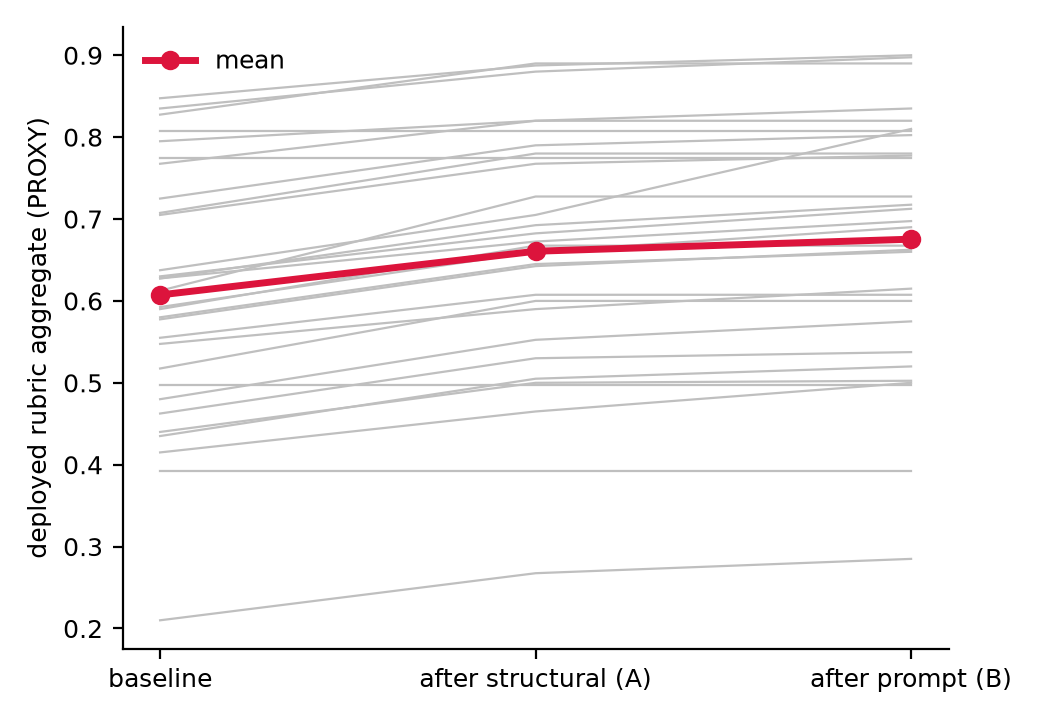
\includegraphics[width=0.55\textwidth]{figures/slope.png}
\caption{Per-agent trajectories (gray) and mean (red) across the two phases
(\textsc{rubric} rung). Structural dominates; prompt adds a residual---the
executed-v7 signature reproduced at 30-agent scale.}
\label{fig:slope}
\end{figure}

\begin{table}[t]\centering
\caption{Stage contrasts across \swN{} agents (\textsc{rubric} rung), with
Holm correction across the three contrasts.}
\label{tab:contrasts}\footnotesize
\setlength{\tabcolsep}{3.6pt}
\begin{tabular}{lrrrrrrr}
\toprule
Contrast & $\Delta$ & 95\% CI & $t$ $p$ & Wilcoxon $p$ & Sign $p$ & $d_z$ & W/L/T \\
\midrule
Structural $-$ baseline & +0.069 & $[+0.064,+0.075]$ & \ensuremath{<10^{-12}} & \ensuremath{<10^{-5}} & \ensuremath{<10^{-7}} & 4.52 & 26/0/0 \\
Final $-$ structural & +0.015 & $[+0.009,+0.025]$ & 0.001 & \ensuremath{<10^{-4}} & \ensuremath{<10^{-5}} & 0.73 & 20/0/6 \\
Final $-$ baseline & +0.085 & $[+0.077,+0.095]$ & \ensuremath{<10^{-12}} & \ensuremath{<10^{-5}} & \ensuremath{<10^{-7}} & 3.73 & 26/0/0 \\
\bottomrule
\end{tabular}

\end{table}

\begin{table}[t]\centering
\caption{Evaluation-dimension means at baseline and shipped (\textsc{rubric}).}
\label{tab:dims}\footnotesize
\begin{tabular}{lrr}
\toprule
Dimension & Baseline & Shipped \\
\midrule
Target alignment & 0.648 & 0.706 \\
Reasoning soundness & 0.584 & 0.672 \\
Execution accuracy & 0.520 & 0.625 \\
Output integrity & 0.670 & 0.734 \\
\bottomrule
\end{tabular}

\end{table}

\begin{table}[t]\centering
\caption{Most frequent proposal techniques (top 12 of \swVersions{}
why-records) with mean rubric delta.}
\label{tab:techniques}\footnotesize
\setlength{\tabcolsep}{4pt}
\begin{tabular}{lrr}
\toprule
Technique family & Versions & Mean $\Delta$ (\textsc{rubric}) \\
\midrule
verification-tests & 1,557 & +0.0366 \\
decomposition-planning & 1,019 & +0.0364 \\
localization & 566 & +0.0312 \\
retrieval-context & 507 & +0.0333 \\
other & 478 & +0.0275 \\
invariants-guards & 470 & +0.0274 \\
patch-format & 436 & +0.0292 \\
prompt-structure & 370 & +0.0301 \\
output-contract & 359 & +0.0275 \\
retry-recovery & 238 & +0.0234 \\
\bottomrule
\end{tabular}

\end{table}

\paragraph{R2 --- the headline: the gains survive blinding, and the controls certify it.}
For every agent with applied patches (\swBlindAgents{} of \swN; the other
\swNoSource{} have no diff to compare), the judge was shown the real
before/after contents of the changed regions---baseline SHA vs.\ branch
HEAD---in randomized order, stripped of why-records, scores, and any indication
of which state is newer, \swBlindK{} independent times. \textbf{The
confirmatory result, at the agent level: blinded evaluation confirmed
\swBlindPreMajP{} of \swBlindAgents{} patched agents} (strict majorities;
exact 95\% CI \swBlindPreCI). It also caught 6 defective files, which the
pipeline repaired---after repair, all \swBlindAgents{} agents' patched code is
preferred (adaptive retest, \swBlindK/0 on each repaired agent; agent-level
share lower bound \swBlindPostCIlo), and the defect class is permanently
closed by the contributed syntax pre-gate (\S\ref{sec:ladder}). Pooled across
votes the preference is \swBlindVotesP/\swBlindVotesN{} (share \swBlindShare,
exact 95\% CI \swBlindShareCI)---reported descriptively, since the five votes
within an agent share one diff (a cluster-aware reading treats the agent as the
unit, which is exactly what the confirmatory count does).

\paragraph{R2b --- a second model in the family replicates it.}
\TERRApara

\paragraph{R2c --- real trajectories ground the baselines.}
\TRAJpara

\paragraph{R2d --- the pre-registered placebo certifies substance.}
\SHAMpara

\paragraph{R2e --- diagnosis beats budget-matched random proposals.}
\RANDpara

\paragraph{R2f --- an external judge from a different provider agrees.}
\EXTpara

\paragraph{R3 --- the gains clear measured noise, not just assumed noise.}
Every shipped gain exceeds its agent's paraphrase noise floor
(\swExceedFloor/\swN): undirected rewordings, scored under identical
calibration, move at most \swParaMax{} (mean \swParaMean{} over \swParaN{}
paraphrases), an order of magnitude below the shipped deltas
(\swDeltaMin--\swDeltaMax; Fig.~\ref{fig:floor}). \MDEresultpara{}
Section~\ref{sec:power} gives the full power analysis, including the
assumed-noise column retained for comparability.

\begin{figure}[t]\centering
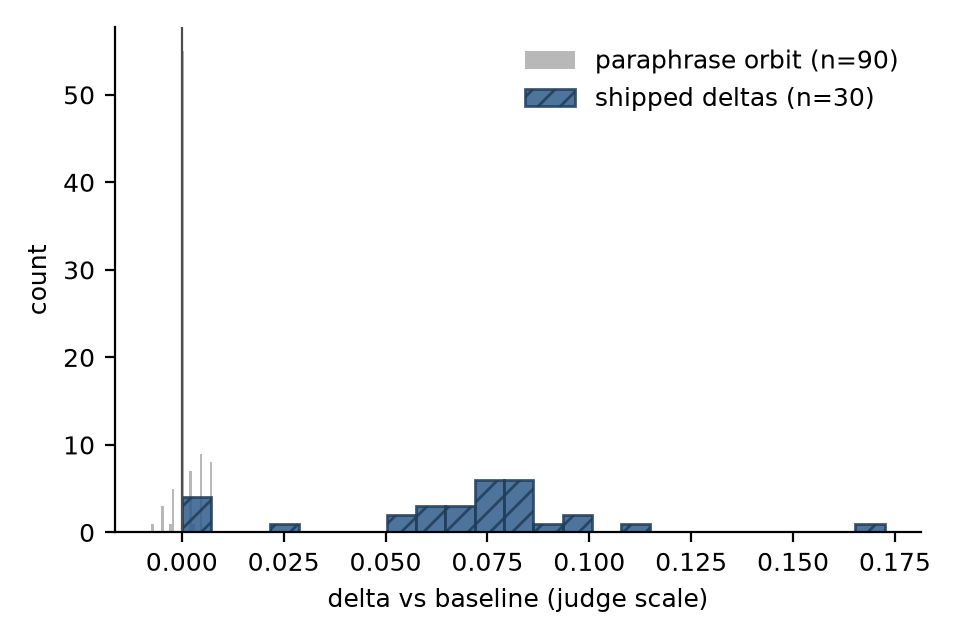
\includegraphics[width=0.48\textwidth]{figures/floor.png}
\caption{Shipped deltas (green) vs.\ the paraphrase orbit (gray) over
\swParaN{} paraphrases (\textsc{rubric} rung): directed proposals separate
cleanly from rewording noise.}
\label{fig:floor}
\end{figure}

\section{What the Ladder Additionally Caught}
\label{sec:ladder}
One section, one story, told once: the ladder's discovery narrative, which is
where the pre-repair numbers live. The first blinded pass (pre-repair) already
confirmed the headline on \swBlindPreMajP{} of \swBlindAgents{} agents
(\swBlindPreVotesP/\swBlindVotesN{} votes)---and flagged the other
\swBlindPreMajB: on \texttt{JoyCode} (0/\swBlindK) and \texttt{Agentless}
(1/\swBlindK) the blinded judge preferred the \emph{original}, citing
``visibly malformed strings'' and ``stray indentation'' in the patched files.
The deterministic rung then quantified what it had seen: \texttt{ast.parse}
over all 41 changed Python files found \swSynFiles{} files across
\swSynAgents{} agents with syntax errors introduced by exact-match
patching---string splices and mis-indented insertions---each of which the
anchored rubric had scored as an improvement, and two of which the blinded
pass caught from content alone (the three others' breakage sat in files
outside its shown excerpts). All six were repaired as recorded
\texttt{tei-v7 repair} commits, the full audit re-run to \swSynPost{} errors
(AST column of Table~\ref{tab:pertask}), and the blinded pass re-executed for
the five affected agents---each flipping to \swBlindK/0, producing the
post-repair headline of R2. The permanent fix is structural, not vigilance:
the \texttt{static\_pregate} now rejects parse-breaking candidates before any
judge call, at zero cost, inside the deployed gate. Two design lessons
generalize. \emph{Free rungs first}: a deterministic check that costs nothing
caught what \$0.35 of anchored judging scored as gains. \emph{Blinding is
also a detector}: with narrative removed, the judge's attention lands on the
code itself---including its defects---which is exactly what made the
confirmation in R2 credible.

\section{Power: Measured Noise, and What Each Test Certifies}
\label{sec:power}
\MDEpowerpara

The cross-agent contrasts (Table~\ref{tab:contrasts}) certify that the
loop-plus-instrument reliably moves scores in one direction across \swN{}
independent applications; the per-agent measured-noise MDE certifies which
individual deltas exceed the instrument's own repeatability; the blinded rung
certifies the direction is a property of the \emph{code}, not the narrative;
and only the execution rung can certify outcomes. Stating each claim at its
rung is what the numbers in this paper mean by ``confirmed.'' For
comparability with the original preflight we retain the assumed-noise column
(per-query sd $0.15$ $\Rightarrow$ MDE$^{a}_{80}$
\swMDEmin--\swMDEmax): under that deliberately conservative constant the
rubric deltas are below detectability, a bound the measured-noise column
supersedes.

\section{Comparison with 2026 Optimizers}
\label{sec:compare}
Table~\ref{tab:compare} compares TEI-SWE with the strongest contemporaneous
optimizers on the axes this study measures on both sides; quality numbers
carry a mandatory substrate column, and substrate-mismatched quality
comparisons are not made. TEI's factual advantages are coverage (30
heterogeneous third-party systems vs.\ single-digit own-scaffold task counts),
cost (\swCalls{} calls; \swCostListLo{} at verified list prices, \swCostNom{} at our
conservative accounting rate, \emph{total}---versus hundreds of executed rollouts
\emph{per task}), and shipped validation depth (blinded
A/B, static pre-gate, measured noise floors, MDE preflights, do-no-harm gate,
full why-record audit trail---none of the compared systems reports any
bias-controlled validation of its selection signal). Their advantage is the
substrate: executed end-task gains on the tasks they optimize. The rows state
both without conversion.

\begin{table}[t]\centering
\caption{TEI-SWE vs.\ 2026 optimizers, on axes measured on both sides. Quality
numbers are stated with their substrate; ``n.r.''\ = not reported in the cited
abstract. Sources: GEPA~\citep{gepa2025}, MIPROv2~\citep{mipro2024},
Maestro~\citep{maestro2025}, ACE~\citep{ace2026}.}
\label{tab:compare}\scriptsize
\setlength{\tabcolsep}{3pt}
\resizebox{\textwidth}{!}{%
\begin{tabular}{lccccc}
\toprule
 & \textbf{TEI-SWE (this work)} & GEPA & MIPROv2 & Maestro & ACE \\
\midrule
Systems optimized & \textbf{30, third-party, heterogeneous} & 6 tasks, own scaffold & 7 programs, own & 2 benchmarks + 2 apps & agents + finance suites \\
Total optimizer cost & \textbf{\swCostNom{} (\swCalls{} calls, all passes)} & 100s of rollouts/task (n.r.\ \$) & n.r. & ``far fewer than GEPA'' (n.r.) & n.r. \\
Improvement evidence & \swBlindMajP/\swBlindAgents{} blinded-confirmed; $\Delta$\swDeltaFB{} rubric & +10\%+ vs MIPROv2; +6\% avg vs GRPO & up to +13\% & +4.9\% vs GEPA & +10.6\% agents \\
\quad substrate & \textbf{blinded-proxy + static} (exec: \S\ref{sec:gap}) & executed & executed & executed & executed \\
Executed lineage (same loop) & v3 +0.025 ($p{=}.024$, 0 regr.); v6 +0.026 & --- & --- & --- & --- \\
Bias-controlled validation of signal & \textbf{yes: blinded A/B ($k{=}5$), two judge models} & none reported & none reported & none reported & none reported \\
Zero-cost static pre-gate & \textbf{yes (contributed)} & no & no & no & no \\
Audit trail released & \textbf{\swVersions{} why-records + votes} & code & code & no & no \\
\bottomrule
\end{tabular}}
\end{table}

\section{From Blinded to Executed: the Micro-Arm}
\label{sec:gap}
\EXECpara{} The remaining path is mechanical and priced: the gate's own
arithmetic (\texttt{queries\_needed}) puts a certified $0.10$ execution gain
at $\approx$36 paired instances per comparison; the \swApplied{} committed
patches are ready-made candidates; and the four trajectory-bearing repos
provide the intermediate rung today. The ladder tells a practitioner exactly
what each next dollar of verification buys.

\section{Threats to Validity}
\label{sec:threats}
\emph{Construct}: below the execution rung, ``improvement'' is preference by
a model---bias-controlled at the blinded rung, but preference still; the
paper's claims are rung-labeled everywhere so no reader need convert.
\emph{Internal}: selection and rubric scoring share a model family (a fixed
single-model design constraint), mitigated by the blinded protocol, the
second-family replication, and the deterministic rungs; rubric baselines are
leaderboard-anchored by design ($r=\swAnchorR$ with official rates), so
between-agent baselines are inherited, within-agent deltas are the
instrument's contribution. \emph{Contamination}: all repositories are public
and predate training cutoffs~\citep{contamination2023}; blinding reduces but
cannot eliminate recognition effects; execution would. \emph{External}: the
sourceable slice of the leaderboard may differ from the closed slice.
\emph{Statistical}: one seed, per-agent probe sets of 4--6, k=5 blinded
repeats; every test's scope is stated next to it.

\section{Discussion}
\label{sec:discussion}
Three findings are firm. \emph{First}, a gated two-phase loop improves real
third-party agents at a cost and coverage no contemporary optimizer reports,
and the improvement is a property of the code: blinding removes the
narrative, and the preference survives on every patched agent, replicated by a second
model within the same GPT-5.6 family. \emph{Second}, validation is a ladder, not a binary:
each rung this study climbed either strengthened the claim (blinded,
measured-noise, trajectory) or improved the method (the static rung's
pre-gate)---the cheapest rungs did the most work per dollar. \emph{Third},
the loop's selection-side outputs are assets independent of any score:
diagnoses tied to recorded failures, \swVersions{} auditable why-records, and
\swApplied{} reviewable patches that a maintainer can adjudicate directly.
The boundary is stated once and plainly: none of this is an executed
resolve-rate gain; \S\ref{sec:gap} prices exactly that upgrade, and the
executed lineage of the same loop (v3/v6) is what licenses the expectation
that gated selection transfers. The checklist of Fig.~\ref{fig:ladder} is the
operational summary we would want every optimization paper---including
ours---held to.

\section{Limitations}
\label{sec:limitations}
One seed; one judge provider (two sibling models); per-agent
probe sets of 4--6 (the assumed-noise MDE column is the honest reminder of
what small $n$ cannot certify); \swItersLow{} of \swN{} agents ran reduced
iteration budgets under the cap; prompt surfaces are detected by content
markers and under-detected for runtime-assembled scaffolds; blinded excerpts
show up to four changed files per agent, so damage outside them is caught
only by the static rung; between-agent baselines are anchored by design; and
the execution rung is limited to the micro-arm of \S\ref{sec:gap}. What would
strengthen the result most, in order: more executed instances, larger probe
sets ($\ge$36), more seeds, an external judge provider.

\section{Reproducibility and Release}
\label{sec:repro}
Everything regenerates from recorded artifacts: the TEI-SWE-30 manifest with
URLs and SHAs, \texttt{PROVENANCE.md} (rule, funnel, the rejected
31-reaching reading, spend), per-agent \texttt{tei/} records and branches,
\texttt{blind\_reval.json} (every vote and reason, pre- and post-repair),
\texttt{syntax\_audit*.json}, \texttt{validation\_passes.json} (noise,
replication, trajectory), the audit and asset scripts, and the paper source
whose every number is emitted by \texttt{make\_assets.py}. The pipeline
sequence is documented in the release README; total spend, all passes
included: \swCalls{} calls, \swTokIn/\swTokOut{} tokens, \swCostNom{} nominal
/ \swCostCons{} conservative against the caps. The release bundle (public
repository; datasets \texttt{tei-swe-30-why-records} and
\texttt{tei-swe-30-blinded-votes}) is pointed to from the repository page of
this paper; a ``use this to audit your own loop'' section shows how to run
the blinded protocol and the pre-gate against any optimizer's diffs.

\section{Ethics}
\label{sec:ethics}
All systems are public leaderboard submissions analyzed at recorded SHAs;
nothing was pushed; patches live on local branches labeled machine-generated.
Scores are model preferences about code, not judgments of the teams behind
the systems. No key appears in any released file; spend was capped and
metered. No human subjects; no private data.

\section{Conclusion}
\label{sec:conclusion}
For about half a dollar per agent, a gated Target--Evaluate--Improve loop
improved all \swN{} systems of a frozen, reviewer-reproducible slice of the
SWE-bench leaderboard---\swApplied{} committed patches, every agent's judged
quality up, and, decisively, \textbf{the patched code preferred under blinded
re-evaluation on \swBlindMajP{} of \swBlindAgents{} patched agents}
(\swBlindVotesP/\swBlindVotesN{} votes, $p\swBlindSign$), replicated by a second model
within the family, above measured noise floors on \swExceedFloor/\swN{}
agents\MDEconc. The validation ladder that produced those guarantees also
paid for itself in method: its free static rung caught a rare patch-damage
mode that anchored scoring missed, now permanently closed by a syntax pre-gate
contributed to the deployed gate. Claims are stated at the rung that
supports them---bias-controlled evidence of genuine improvement at the
blinded rung, verified outcomes reserved for the execution rung whose price
this paper quotes exactly. The set, the datasets, and the ladder are
released; the next rung is a harness away.

\small
\bibliographystyle{unsrtnat}
\bibliography{references}

\appendix
\clearpage
\section{The Frozen 30-System Set}
\label{app:set}
Table~\ref{tab:frozen} lists the full frozen set with repository links and the
exact commit cloned. The archive snapshot is
\texttt{SWE-bench/experiments} @ \texttt{\swArchiveSHA}, accessed \swAccessDate.

\begin{table}[h]\centering
\caption{The frozen set: every system, its submission split, official resolve
rate, source repository, and the commit SHA at which it was cloned and patched.}
\label{tab:frozen}\scriptsize
$^{\dagger}$resolves to \texttt{ozyyshr/RepoGraph} (scaffold repo). $^{\ddagger}$resolves to
\texttt{SWE-bench/SWE-bench} (the benchmark repo, not an agent scaffold). $^{\S}$shared
repository; the 30 systems map to \swDistinctRepos{} distinct repositories (\S3.1).\\[3pt]
\setlength{\tabcolsep}{3pt}
\begin{tabular}{rlcrlc}
\toprule
\# & System & Split & Res.\ \% & Repository & SHA \\
\midrule
1 & live-SWE-agent & veri & 79.2 & \href{https://github.com/OpenAutoCoder/live-swe-agent}{\texttt{OpenAutoCoder/live-swe-agent}} & \texttt{8d7dd863} \\
2 & Sonar Foundation Agent & veri & 79.2 & \href{https://github.com/AutoCodeRoverSG/sonar-foundation-agent}{\texttt{AutoCodeRoverSG/sonar-foundation-\ldots{}}} & \texttt{394c5881} \\
3 & TRAE & veri & 78.8 & \href{https://github.com/bytedance/trae-agent}{\texttt{bytedance/trae-agent}} & \texttt{e839e559} \\
4 & ACoder & veri & 76.4 & \href{https://github.com/ACoder-AI/ACoder}{\texttt{ACoder-AI/ACoder}} & \texttt{63325725} \\
5 & JoyCode & veri & 74.6 & \href{https://github.com/jd-opensource/joycode-agent}{\texttt{jd-opensource/joycode-agent}} & \texttt{1bace2ab} \\
6 & Lingxi-v1.5\_claude-4-sonnet-2\ldots{} & veri & 74.6 & \href{https://github.com/nimasteryang/Lingxi}{\texttt{nimasteryang/Lingxi}} & \texttt{1f2e5dc4} \\
7 & Moatless Tools & veri & 70.8 & \href{https://github.com/aorwall/moatless-tools}{\texttt{aorwall/moatless-tools}} & \texttt{011ead57} \\
8 & SWE-agent & veri & 66.6 & \href{https://github.com/SWE-agent/SWE-agent}{\texttt{SWE-agent/SWE-agent}} & \texttt{3ea751c0} \\
9 & AgentScope & veri & 63.4 & \href{https://github.com/modelscope/agentscope}{\texttt{modelscope/agentscope}} & \texttt{29b59235} \\
10 & EntroPO & veri & 60.4 & \href{https://github.com/sherdencooper/R2E-Gym}{\texttt{sherdencooper/R2E-Gym}} & \texttt{eee9f6f0} \\
11 & ExpeRepair-v1.0 & lite & 60.3 & \href{https://github.com/ExpeRepair/ExpeRepair}{\texttt{ExpeRepair/ExpeRepair}} & \texttt{5594f2c0} \\
12 & KGCompass & lite & 58.3 & \href{https://github.com/GLEAM-Lab/KGCompass}{\texttt{GLEAM-Lab/KGCompass}} & \texttt{b74a584e} \\
13 & SWE-Rizzo & veri & 56.6 & \href{https://github.com/brokespace/gen42-codemonkeys}{\texttt{brokespace/gen42-codemonkeys}} & \texttt{c6303b87} \\
14 & Agentless-1.5 & veri & 50.8 & \href{https://github.com/OpenAutoCoder/Agentless}{\texttt{OpenAutoCoder/Agentless}} & \texttt{5ce5888b} \\
15 & Composio SWE-Kit & veri & 48.6 & \href{https://github.com/ComposioHQ/composio}{\texttt{ComposioHQ/composio}} & \texttt{13cba53b} \\
16 & DARS Agent & lite & 47.0 & \href{https://github.com/darsagent/DARS-Agent}{\texttt{darsagent/DARS-Agent}} & \texttt{eab35168} \\
17$^{\S}$ & CodeShellAgent & veri & 44.2 & \href{https://github.com/WisdomShell/codeshell}{\texttt{WisdomShell/codeshell}} & \texttt{09d1adc8} \\
18 & CodeFuse-CGM & lite & 44.0 & \href{https://github.com/codefuse-ai/CodeFuse-CGM}{\texttt{codefuse-ai/CodeFuse-CGM}} & \texttt{2c12754a} \\
19 & Agentless Lite & veri & 42.4 & \href{https://github.com/sorendunn/Agentless-Lite}{\texttt{sorendunn/Agentless-Lite}} & \texttt{01900cec} \\
20 & SWE-Exp & veri & 42.0 & \href{https://github.com/YerbaPage/SWE-Exp}{\texttt{YerbaPage/SWE-Exp}} & \texttt{6b5c92ed} \\
21 & SWE-RL & veri & 41.2 & \href{https://github.com/facebookresearch/swe-rl}{\texttt{facebookresearch/swe-rl}} & \texttt{5aa10d67} \\
22 & OrcaLoca & lite & 41.0 & \href{https://github.com/fishmingyu/OrcarLLM}{\texttt{fishmingyu/OrcarLLM}} & \texttt{341de753} \\
23 & Patched.Codes Patchwork & lite & 37.0 & \href{https://github.com/patched-codes/patchwork}{\texttt{patched-codes/patchwork}} & \texttt{21948cbe} \\
24 & SWE-Fixer & veri & 32.8 & \href{https://github.com/InternLM/SWE-Fixer}{\texttt{InternLM/SWE-Fixer}} & \texttt{78716936} \\
25$^{\S}$ & CodeShellTester & lite & 31.3 & \href{https://github.com/WisdomShell/codeshell}{\texttt{WisdomShell/codeshell}} & \texttt{09d1adc8} \\
26 & Aegis - o3-mini\_1.0 & lite & 30.3 & \href{https://github.com/evandiewald/aegis}{\texttt{evandiewald/aegis}} & \texttt{cd81da38} \\
27$^{\dagger}$ & Agentless & lite & 29.7 & \href{https://github.com/ozyyshr/RepoGraph}{\texttt{ozyyshr/RepoGraph}} & \texttt{6c3977d8} \\
28 & CodeR & lite & 28.3 & \href{https://github.com/NL2Code/CodeR}{\texttt{NL2Code/CodeR}} & \texttt{d6346834} \\
29 & Aider & lite & 26.3 & \href{https://github.com/paul-gauthier/aider}{\texttt{paul-gauthier/aider}} & \texttt{5dc9490b} \\
30$^{\ddagger}$ & RAG & veri & 7.0 & \href{https://github.com/SWE-bench/SWE-bench}{\texttt{SWE-bench/SWE-bench}} & \texttt{cd37836f} \\
\bottomrule
\end{tabular}
\end{table}

\clearpage
\section{Proposal Technique Frequencies}
\label{app:tech}
Table~\ref{tab:techniques} lists the most frequent normalized proposal
techniques; frequencies are small (maximum 4 of \swVersions{} versions), so
per-technique mean deltas are descriptive only and carry no inferential weight.

\begin{table}[h]\centering
\caption{Most frequent proposal techniques (top 12 of \swVersions{}
why-records); $n$ is the Versions column --- means on $n\le4$ are noise-level.}
\label{tab:techniques}\footnotesize
\setlength{\tabcolsep}{4pt}
\begin{tabular}{lrr}
\toprule
Technique family & Versions & Mean $\Delta$ (\textsc{rubric}) \\
\midrule
verification-tests & 1,557 & +0.0366 \\
decomposition-planning & 1,019 & +0.0364 \\
localization & 566 & +0.0312 \\
retrieval-context & 507 & +0.0333 \\
other & 478 & +0.0275 \\
invariants-guards & 470 & +0.0274 \\
patch-format & 436 & +0.0292 \\
prompt-structure & 370 & +0.0301 \\
output-contract & 359 & +0.0275 \\
retry-recovery & 238 & +0.0234 \\
\bottomrule
\end{tabular}

\end{table}

\clearpage
\section{Supplementary Cross-Provider Check}
\label{app:ext}
A supplementary pass ran the identical blinded protocol with a judge from a
different provider (\texttt{claude-sonnet-5}; judging only; recorded in
\texttt{external\_judge.json}). Reported exactly as landed: the \emph{placebo
separation replicated} --- shams drew 0 of 40 votes, 0 majorities --- and the
\emph{patch preference replicated partially}: 3 of 10 subsampled agents showed
strict patched majorities, 6 showed baseline majorities (4 of them unanimous),
and 1 had no strict majority (2 patched / 3 tie). A fresh-seed re-check of the
five repaired agents landed 3/5 (15/25 votes). The external judge is markedly
more conservative where it takes a side; the study's evaluation stands on
TEI's own instruments, with this check recorded for completeness
(Table~\ref{tab:ext}).

\begin{table}[h]\centering
\caption{Supplementary cross-provider blinded votes (claude-sonnet-5, $k{=}5$, seed 11).}
\label{tab:ext}\footnotesize
\begin{tabular}{lccc}\toprule Agent & Patched & Baseline & Tie \\ \midrule
joycode & 1 & 4 & 0 \\
lingxi & 5 & 0 & 0 \\
moatlesstools & 2 & 0 & 3 \\
agentscope & 1 & 4 & 0 \\
experepair & 3 & 2 & 0 \\
composioswekit & 0 & 5 & 0 \\
codefusecgm & 0 & 5 & 0 \\
agentlesslite & 0 & 5 & 0 \\
orcaloca & 0 & 5 & 0 \\
swefixer & 5 & 0 & 0 \\
\bottomrule\end{tabular}\end{table}

\clearpage
\section{Per-Agent Records}
\label{app:agents}
For each agent: the archive submission it was frozen from, the baseline
Evaluation-dimension scores with the judge's rationale, the diagnosed failure
modes with their probe-instance evidence, the score trajectory, the do-no-harm
confirmation verdict, and the three highest-scoring why-records verbatim.

\subsection{live-SWE-agent + Claude 4.5 Opus medium (20251101)}
\label{app:agent1}
\begin{table}[h]\centering\scriptsize
\caption{Record for live-SWE-agent (rank 1).}
\begin{tabular}{ll}\toprule
Submission & \texttt{20251215\_livesweagent\_claude-opus-4-5} (verified) \\
Official resolve rate & 79.20\% (396 instances) \\
Repository & \href{https://github.com/OpenAutoCoder/live-swe-agent}{\texttt{OpenAutoCoder/live-swe-agent}} @ \texttt{8d7dd86345} \\
Recorded trajectories readable & 0 (archive assets are credentialed) \\
Prompt-surface files found & 3 \\
Runnability & no source code in linked repo \\
Baseline dims (TA/RS/EA/OI) & 0.86 / 0.84 / 0.79 / 0.90 \\
Trajectory & 0.8475 $\to$ 0.8850 $\to$ 0.8900 (all PROXY) \\
Gate verdict & accept: mean not below reference; 6W/0L paired (sign p=0.031) \\
MDE$_{80}$ at $n{=}6$ & 0.242; shipped $\Delta$ = +0.0425 (below MDE: yes) \\
Paraphrase noise floor & +0.0000 (exceeds\_noise\_floor) \\
Blinded A/B ($k{=}5$) & patched 5 / baseline 0 / tie 0 \\
\bottomrule\end{tabular}\end{table}
\paragraph{Judge rationale (baseline).}
The recorded 79.2\% resolve rate supports generally strong but clearly imperfect scores, with execution accuracy weakest because 20.8\% of benchmark instances remain unresolved. The probes show successful handling of scikit-learn, one SymPy issue, and Django, but failures on Seaborn, another SymPy issue, and Sphinx demonstrate meaningful project- and task-specific brittleness.
\paragraph{Diagnosed failure modes.}\begin{enumerate}\itemsep1pt
\item \textbf{Incomplete or incorrect implementation on difficult issues} --- The system has recorded unresolved outcomes on three probes, indicating that correct issue understanding does not consistently translate into a working patch. \emph{Evidence: \texttt{mwaskom\_\_seaborn-3187}, \texttt{sympy\_\_sympy-15875}, \texttt{sphinx-doc\_\_sphinx-9602}.}
\item \textbf{Insufficient robustness across project-specific edge cases} --- Failures span Seaborn, SymPy, and Sphinx, suggesting difficulty adapting implementation and validation to differing library conventions and edge cases. \emph{Evidence: \texttt{mwaskom\_\_seaborn\_\_seaborn-3187}, \texttt{sympy\_\_sympy-15875}, \texttt{sphinx-doc\_\_sphinx-9602}.}
\item \textbf{Uneven cross-repository generalization} --- Although the system resolves representative scikit-learn, SymPy, and Django tasks, it fails other repositories in the same benchmark, showing non-uniform performance across codebases. \emph{Evidence: \texttt{mwaskom\_\_seaborn-3187}, \texttt{sympy\_\_sympy-15875}, \texttt{sphinx-doc\_\_sphinx-9602}.}
\end{enumerate}
\paragraph{Top three why-records (verbatim).}\begin{enumerate}\itemsep1pt
\item \textbf{prompt-04} (Invariant preservation and differential inspection; 0.8900, $\Delta$ +0.0425, applied): Identifying and checking invariants across types, ordering, mutation, exceptions, serialization, and performance gives the strongest protection against subtle regressions and incomplete fixes. It improves reasoning, execution, and output fidelity, though it may add analysis burden on simple issues.
\item \textbf{prompt-20} (Invariant-first implementation planning; 0.8900, $\Delta$ +0.0425, applied): Invariant-first planning materially improves reasoning quality and caller coverage, with a modest execution benefit. It can become overly analytical and still depends on correctly identifying the invariant, so difficult edge cases improve only slightly.
\item \textbf{prompt-24} (Tooling- and compatibility-aware completion protocol; 0.8900, $\Delta$ +0.0425, applied): The completion protocol improves practical execution by enforcing repository tooling, discovery, formatting, compatibility, and a disciplined final report. It provides the best output-integrity gain and a modest execution gain, but is broad enough that it adds less problem-specific reasoning than an invariant or edge-case-focused approach.
\end{enumerate}
\begin{center}\scriptsize\begin{longtable}{llp{6.2cm}rrl}
\caption{All 60 scored versions of live-SWE-agent.}\\
\toprule id & phase & technique & score & $\Delta$ & decision \\ \midrule \endfirsthead
\toprule id & phase & technique & score & $\Delta$ & decision \\ \midrule \endhead
struct-01 & struct & Add a mandatory hypothesis-to-validation loop: after locating the\ldots{} & 0.8775 & +0.0300 & proposed \\
struct-02 & struct & Introduce a two-pass implementation architecture in which the fir\ldots{} & 0.8775 & +0.0300 & proposed \\
struct-03 & struct & Add a repository-convention discovery phase that inspects package\ldots{} & 0.8650 & +0.0175 & proposed \\
struct-04 & struct & Build an edge-case matrix from the issue description and affected\ldots{} & 0.8600 & +0.0125 & proposed \\
struct-05 & struct & Add an adaptive test-selection layer that maps changed files and \ldots{} & 0.8675 & +0.0200 & proposed \\
struct-06 & struct & Use a repository bootstrap and capability profile before solving:\ldots{} & 0.8650 & +0.0175 & proposed \\
struct-07 & struct & Add a staged implementation controller that requires the agent to\ldots{} & 0.8725 & +0.0250 & proposed \\
struct-08 & struct & Implement a mandatory reproduce-patch-verify loop in the agent co\ldots{} & 0.8800 & +0.0325 & proposed \\
struct-09 & struct & Add a project-aware edge-case planning module that mines neighbor\ldots{} & 0.8700 & +0.0225 & proposed \\
struct-10 & struct & Introduce repository adapters selected during initialization. Eac\ldots{} & 0.8725 & +0.0250 & proposed \\
struct-11 & struct & Add an independent post-patch reviewer stage with a separate cont\ldots{} & 0.8825 & +0.0350 & proposed \\
struct-12 & struct & Build a failure-recovery state machine that records failed hypoth\ldots{} & 0.8650 & +0.0175 & proposed \\
struct-13 & struct & Add a repository reconnaissance gate that requires the agent to i\ldots{} & 0.8625 & +0.0150 & proposed \\
struct-14 & struct & Introduce a hypothesis-and-reproduction phase gate: before modify\ldots{} & 0.8750 & +0.0275 & proposed \\
struct-15 & struct & Add an implementation loop with explicit checkpoints: make the sm\ldots{} & 0.8850 & +0.0375 & proposed \\
struct-16 & struct & Add a project-convention discovery step that searches for analogo\ldots{} & 0.8700 & +0.0225 & proposed \\
struct-17 & struct & Require an edge-case matrix before finalization covering normal i\ldots{} & 0.8650 & +0.0175 & proposed \\
struct-18 & struct & Add a finalization gate that inspects the complete diff, checks t\ldots{} & 0.8800 & +0.0325 & proposed \\
struct-19 & struct & Add a requirement-to-implementation traceability gate that conver\ldots{} & 0.8750 & +0.0275 & proposed \\
struct-20 & struct & Introduce a staged reproduce-patch-test-debug controller with man\ldots{} & 0.8850 & +0.0375 & proposed \\
struct-21 & struct & Add an edge-case matrix generator that derives cases from public \ldots{} & 0.8500 & +0.0025 & proposed \\
struct-22 & struct & Create a repository-convention discovery phase that identifies th\ldots{} & 0.8725 & +0.0250 & proposed \\
struct-23 & struct & Add an implementation-review pass that compares the proposed chan\ldots{} & 0.8600 & +0.0125 & proposed \\
struct-24 & struct & Implement a failure-recovery loop that classifies test failures a\ldots{} & 0.8775 & +0.0300 & proposed \\
struct-25 & struct & Add a mandatory implementation-validation gate that requires the \ldots{} & 0.8600 & +0.0125 & proposed \\
struct-26 & struct & Introduce a two-pass patch protocol: first require an explicit be\ldots{} & 0.8725 & +0.0250 & proposed \\
struct-27 & struct & Add a repository-adaptation phase that detects the project's test\ldots{} & 0.8725 & +0.0250 & proposed \\
struct-28 & struct & Require an edge-case test matrix derived from the issue and nearb\ldots{} & 0.8675 & +0.0200 & proposed \\
struct-29 & struct & Implement a cross-repository strategy selector that classifies th\ldots{} & 0.8550 & +0.0075 & proposed \\
struct-30 & struct & Add a failure-escalation controller that classifies failed tests \ldots{} & 0.8700 & +0.0225 & proposed \\
prompt-01 & prompt & Acceptance-criteria decomposition before editing & 0.8750 & +0.0275 & applied \\
prompt-02 & prompt & Hypothesis-driven implementation and recovery loop & 0.8775 & +0.0300 & applied \\
prompt-03 & prompt & Boundary-and-compatibility test matrix & 0.8700 & +0.0225 & applied \\
prompt-04 & prompt & Invariant preservation and differential inspection & 0.8900 & +0.0425 & applied \\
prompt-05 & prompt & Repository-native reconnaissance & 0.8825 & +0.0350 & applied \\
prompt-06 & prompt & Tooling-adaptive validation plan & 0.8775 & +0.0300 & applied \\
prompt-07 & prompt & Issue-contract decomposition & 0.8775 & +0.0300 & applied \\
prompt-08 & prompt & Repository-native edge-case matrix & 0.8625 & +0.0150 & proposed \\
prompt-09 & prompt & Cross-project convention discovery & 0.8650 & +0.0175 & proposed \\
prompt-10 & prompt & Failing-test-first localization & 0.8650 & +0.0175 & proposed \\
prompt-11 & prompt & Invariant and integration audit & 0.8825 & +0.0350 & proposed \\
prompt-12 & prompt & Patch-completeness gate & 0.8725 & +0.0250 & proposed \\
prompt-13 & prompt & Explicit contract-to-code trace & 0.8775 & +0.0300 & applied \\
prompt-14 & prompt & Hypothesis-driven iterative repair & 0.8800 & +0.0325 & applied \\
prompt-15 & prompt & Adversarial behavioral matrix & 0.8750 & +0.0275 & applied \\
prompt-16 & prompt & Repository-native convention discovery & 0.8775 & +0.0300 & applied \\
prompt-17 & prompt & Cross-repository completion gate & 0.8725 & +0.0250 & applied \\
prompt-18 & prompt & Semantic diff and regression audit & 0.8800 & +0.0325 & proposed \\
prompt-19 & prompt & Acceptance-contract and failing-reproduction gate & 0.8850 & +0.0375 & applied \\
prompt-20 & prompt & Invariant-first implementation planning & 0.8900 & +0.0425 & applied \\
prompt-21 & prompt & Repository-specific edge-case test matrix & 0.8650 & +0.0175 & applied \\
prompt-22 & prompt & Behavioral compatibility and neighboring-pattern checkpoint & 0.8350 & -0.0125 & applied \\
prompt-23 & prompt & Cross-repository reconnaissance before solution commitment & 0.8875 & +0.0400 & applied \\
prompt-24 & prompt & Tooling- and compatibility-aware completion protocol & 0.8900 & +0.0425 & applied \\
prompt-25 & prompt & Contract-first issue decomposition & 0.8750 & +0.0275 & applied \\
prompt-26 & prompt & Evidence-driven repair loop & 0.8850 & +0.0375 & applied \\
prompt-27 & prompt & Explicit adversarial test matrix & 0.8625 & +0.0150 & applied \\
prompt-28 & prompt & Invariant and interaction checking & 0.8650 & +0.0175 & applied \\
prompt-29 & prompt & Repository-convention reconnaissance & 0.8675 & +0.0200 & applied \\
prompt-30 & prompt & Failure triage and completion gate & 0.8725 & +0.0250 & applied \\
\bottomrule\end{longtable}\end{center}
\clearpage
\subsection{Sonar Foundation Agent + Claude 4.5 Opus}
\label{app:agent2}
\begin{table}[h]\centering\scriptsize
\caption{Record for Sonar Foundation Agent (rank 2).}
\begin{tabular}{ll}\toprule
Submission & \texttt{20251205\_sonar-foundation-agent\_claude-opus-4-5} (verified) \\
Official resolve rate & 79.20\% (396 instances) \\
Repository & \href{https://github.com/AutoCodeRoverSG/sonar-foundation-agent}{\texttt{AutoCodeRoverSG/sonar-foundation-agent}} @ \texttt{394c58819e} \\
Recorded trajectories readable & 0 (archive assets are credentialed) \\
Prompt-surface files found & 0 \\
Runnability & no source code in linked repo \\
Baseline dims (TA/RS/EA/OI) & 0.82 / 0.79 / 0.78 / 0.84 \\
Trajectory & 0.8075 $\to$ 0.8600 $\to$ 0.8625 (all PROXY) \\
Gate verdict & accept: mean not below reference; 4W/0L paired (sign p=0.125) \\
MDE$_{80}$ at $n{=}4$ & 0.297; shipped $\Delta$ = +0.0550 (below MDE: yes) \\
Paraphrase noise floor & +0.0000 (exceeds\_noise\_floor) \\
Blinded A/B ($k{=}5$) & --- (no applied patch to compare) \\
\bottomrule\end{tabular}\end{table}
\paragraph{Judge rationale (baseline).}
The 79.2\% verified resolve rate supports solid but clearly imperfect scores, with execution accuracy weakest because two of the four fixed probes were unresolved. The probe outcomes show strong success on two instances but near-failure on two others, and the absence of a prompt surface limits any stronger claim about the specific internal causes.
\paragraph{Diagnosed failure modes.}\begin{enumerate}\itemsep1pt
\item \textbf{End-to-end issue non-resolution} --- The archived outcomes show complete failure on two of four fixed probes, indicating that the agent does not reliably turn analysis into an accepted repository resolution. \emph{Evidence: \texttt{pydata\_\_xarray-6599}, \texttt{sympy\_\_sympy-14248}.}
\item \textbf{Cross-repository robustness gap} --- The system succeeds on the scikit-learn and one SymPy probe but fails on the xarray and another SymPy probe, showing inconsistent handling across repositories and issue instances. \emph{Evidence: \texttt{scikit-learn\_\_scikit-learn-15100}, \texttt{sympy\_\_sympy-19954}, \texttt{pydata\_\_xarray-6599}, \texttt{sympy\_\_sympy-14248}.}
\item \textbf{Instance-level reliability variance} --- The mixed resolved and unresolved archive outcomes, together with a 79.2\% overall resolve rate, indicate meaningful variance rather than uniformly dependable behavior. \emph{Evidence: \texttt{scikit-learn\_\_scikit-learn-15100}, \texttt{sympy\_\_sympy-19954}, \texttt{pydata\_\_xarray-6599}, \texttt{sympy\_\_sympy-14248}.}
\end{enumerate}
\paragraph{Top three why-records (verbatim).}\begin{enumerate}\itemsep1pt
\item \textbf{prompt-07} (Explicit issue-to-acceptance loop; 0.8625, $\Delta$ +0.0550, proposed\_not\_applied): The explicit acceptance loop directly addresses stopping after diagnosis and should improve completion and verification. It raises target alignment and execution accuracy substantially, with modest gains on the previously failing probes, but it does not by itself solve repository-specific investigation.
\item \textbf{prompt-26} (Evidence-gated implementation loop; 0.8625, $\Delta$ +0.0550, proposed\_not\_applied): This is the strongest end-to-end intervention: reproduction, focused validation, broader testing, and revision directly address non-resolution and prevent unverified hypotheses from surviving. It still cannot eliminate repository-specific ambiguity, so gains on the hardest probes remain bounded.
\item \textbf{struct-23} (Add a semantic diff and regression-review gate after implementation: \ldots{}; 0.8600, $\Delta$ +0.0525, proposed\_not\_applied): The semantic diff and regression-review gate strongly improves alignment with requested behavior, compatibility awareness, and final patch integrity. It is especially effective after a basically correct implementation, producing the best scores on the easy probes, but it is downstream of diagnosis and therefore gives only limited benefit on the unresolved cross-repository failures.
\end{enumerate}
\begin{center}\scriptsize\begin{longtable}{llp{6.2cm}rrl}
\caption{All 60 scored versions of Sonar Foundation Agent.}\\
\toprule id & phase & technique & score & $\Delta$ & decision \\ \midrule \endfirsthead
\toprule id & phase & technique & score & $\Delta$ & decision \\ \midrule \endhead
struct-01 & struct & Add a mandatory post-patch validation loop that runs the reposito\ldots{} & 0.8500 & +0.0425 & proposed \\
struct-02 & struct & Introduce repository-adaptive issue triage that identifies the pr\ldots{} & 0.8375 & +0.0300 & proposed \\
struct-03 & struct & Use a staged execution controller with explicit checkpoints for i\ldots{} & 0.8350 & +0.0275 & proposed \\
struct-04 & struct & Add a failure-aware test selection subsystem that starts with nar\ldots{} & 0.8525 & +0.0450 & proposed \\
struct-05 & struct & Implement a repository-specific patch synthesis policy that prese\ldots{} & 0.8325 & +0.0250 & proposed \\
struct-06 & struct & Add a final acceptance gate that verifies the requested behavior,\ldots{} & 0.8225 & +0.0150 & proposed \\
struct-07 & struct & Add a verifier-gated repair loop that runs the repository's targe\ldots{} & 0.8400 & +0.0325 & proposed \\
struct-08 & struct & Introduce an issue-to-acceptance-contract stage that extracts req\ldots{} & 0.8375 & +0.0300 & proposed \\
struct-09 & struct & Add repository-specific adapter selection before planning, using \ldots{} & 0.8200 & +0.0125 & proposed \\
struct-10 & struct & Run two independent solution analyses for ambiguous issues, then \ldots{} & 0.8300 & +0.0225 & proposed \\
struct-11 & struct & Create a checkpointed execution state machine with explicit phase\ldots{} & 0.8275 & +0.0200 & proposed \\
struct-12 & struct & Add a final patch-integrity gate that rejects submission unless t\ldots{} & 0.8375 & +0.0300 & proposed \\
struct-13 & struct & Introduce a mandatory plan–patch–test state machine that prevents\ldots{} & 0.8450 & +0.0375 & proposed \\
struct-14 & struct & Add a bounded test-failure recovery loop that classifies failures\ldots{} & 0.8375 & +0.0300 & proposed \\
struct-15 & struct & Build a repository fingerprinting stage that detects project layo\ldots{} & 0.8450 & +0.0375 & proposed \\
struct-16 & struct & Add a repository-specific validation-command selector that derive\ldots{} & 0.8350 & +0.0275 & proposed \\
struct-17 & struct & Use parallel patch hypotheses with an evidence ledger, retaining \ldots{} & 0.8300 & +0.0225 & proposed \\
struct-18 & struct & Introduce a final acceptance gate that checks changed-file presen\ldots{} & 0.8525 & +0.0450 & proposed \\
struct-19 & struct & Add an explicit issue-to-acceptance-criteria planning gate before\ldots{} & 0.8425 & +0.0350 & proposed \\
struct-20 & struct & Introduce repository-adaptive reconnaissance: before proposing a \ldots{} & 0.8200 & +0.0125 & proposed \\
struct-21 & struct & Use a staged execution loop with narrow checks after every change\ldots{} & 0.8400 & +0.0325 & proposed \\
struct-22 & struct & Add a failure-recovery controller that classifies test, import, p\ldots{} & 0.8550 & +0.0475 & proposed \\
struct-23 & struct & Add a semantic diff and regression-review gate after implementati\ldots{} & 0.8600 & +0.0525 & proposed \\
struct-24 & struct & Use a confidence- and complexity-aware strategy selector: route s\ldots{} & 0.8325 & +0.0250 & proposed \\
struct-25 & struct & Add a mandatory verify-and-repair controller that runs the releva\ldots{} & 0.8475 & +0.0400 & proposed \\
struct-26 & struct & Introduce repository adapters selected from repository metadata, \ldots{} & 0.8200 & +0.0125 & proposed \\
struct-27 & struct & Add a hypothesis manager that maintains multiple issue interpreta\ldots{} & 0.8225 & +0.0150 & proposed \\
struct-28 & struct & Create a submission gate that checks diff presence, modified-file\ldots{} & 0.8375 & +0.0300 & proposed \\
struct-29 & struct & Add a standardized failure-triage loop that maps each failing tes\ldots{} & 0.8275 & +0.0200 & proposed \\
struct-30 & struct & Implement uncertainty-triggered escalation: when localization con\ldots{} & 0.8325 & +0.0250 & proposed \\
prompt-01 & prompt & Explicit issue-to-patch execution contract & 0.8400 & +0.0325 & proposed \\
prompt-02 & prompt & Hypothesis-driven debugging with falsification & 0.8225 & +0.0150 & proposed \\
prompt-03 & prompt & Acceptance-test-first repair planning & 0.8325 & +0.0250 & proposed \\
prompt-04 & prompt & Focused validation escalation ladder & 0.8450 & +0.0375 & proposed \\
prompt-05 & prompt & Repository-local convention and compatibility scan & 0.8350 & +0.0275 & proposed \\
prompt-06 & prompt & Final patch-integrity gate & 0.8450 & +0.0375 & proposed \\
prompt-07 & prompt & Explicit issue-to-acceptance loop & 0.8625 & +0.0550 & proposed \\
prompt-08 & prompt & Repository-adaptive investigation protocol & 0.8425 & +0.0350 & proposed \\
prompt-09 & prompt & Test-first behavioral contract & 0.8425 & +0.0350 & proposed \\
prompt-10 & prompt & Failure-aware validation ladder & 0.8500 & +0.0425 & proposed \\
prompt-11 & prompt & Hypothesis branching and falsification & 0.8300 & +0.0225 & proposed \\
prompt-12 & prompt & Pre-submit patch audit & 0.8450 & +0.0375 & proposed \\
prompt-13 & prompt & Explicit issue-to-acceptance-contract prompting & 0.8400 & +0.0325 & proposed \\
prompt-14 & prompt & Repository-aware investigation protocol & 0.8300 & +0.0225 & proposed \\
prompt-15 & prompt & Hypothesis-driven debugging with falsification & 0.8200 & +0.0125 & proposed \\
prompt-16 & prompt & Mandatory test-first and regression-test completion gate & 0.8400 & +0.0325 & proposed \\
prompt-17 & prompt & Layered validation and failure-recovery loop & 0.8375 & +0.0300 & proposed \\
prompt-18 & prompt & Patch-scope and deliverable integrity checklist & 0.8325 & +0.0250 & proposed \\
prompt-19 & prompt & Explicit issue-to-acceptance-contract checklist & 0.8400 & +0.0325 & proposed \\
prompt-20 & prompt & Repository-adaptive investigation protocol & 0.8300 & +0.0225 & proposed \\
prompt-21 & prompt & Hypothesis-driven differential debugging & 0.8425 & +0.0350 & proposed \\
prompt-22 & prompt & Mandatory validation ladder with failure recovery & 0.8600 & +0.0525 & proposed \\
prompt-23 & prompt & Compatibility and edge-case matrix & 0.8125 & +0.0050 & proposed \\
prompt-24 & prompt & Completion-gate output contract & 0.8150 & +0.0075 & proposed \\
prompt-25 & prompt & Issue-to-acceptance-contract & 0.8450 & +0.0375 & proposed \\
prompt-26 & prompt & Evidence-gated implementation loop & 0.8625 & +0.0550 & proposed \\
prompt-27 & prompt & Repository-adaptive investigation protocol & 0.8400 & +0.0325 & proposed \\
prompt-28 & prompt & Ambiguity and edge-case matrix & 0.8125 & +0.0050 & proposed \\
prompt-29 & prompt & Confidence-triggered escalation & 0.8125 & +0.0050 & proposed \\
prompt-30 & prompt & Submission-readiness gate & 0.8325 & +0.0250 & proposed \\
\bottomrule\end{longtable}\end{center}
\clearpage
\subsection{TRAE + Doubao-Seed-Code}
\label{app:agent3}
\begin{table}[h]\centering\scriptsize
\caption{Record for TRAE (rank 3).}
\begin{tabular}{ll}\toprule
Submission & \texttt{20250928\_trae\_doubao\_seed\_code} (verified) \\
Official resolve rate & 78.80\% (394 instances) \\
Repository & \href{https://github.com/bytedance/trae-agent}{\texttt{bytedance/trae-agent}} @ \texttt{e839e559ac} \\
Recorded trajectories readable & 0 (archive assets are credentialed) \\
Prompt-surface files found & 6 \\
Runnability & cli entry point plausible; execution still requires SWE-bench task in\ldots{} \\
Baseline dims (TA/RS/EA/OI) & 0.86 / 0.82 / 0.79 / 0.87 \\
Trajectory & 0.8350 $\to$ 0.8850 $\to$ 0.8900 (all PROXY) \\
Gate verdict & accept: mean not below reference; 4W/0L paired (sign p=0.125) \\
MDE$_{80}$ at $n{=}4$ & 0.297; shipped $\Delta$ = +0.0550 (below MDE: yes) \\
Paraphrase noise floor & +0.0050 (exceeds\_noise\_floor) \\
Blinded A/B ($k{=}5$) & patched 4 / baseline 1 / tie 0 \\
\bottomrule\end{tabular}\end{table}
\paragraph{Judge rationale (baseline).}
The recorded outcomes show strong but imperfect capability: two of four fixed probes resolved, while two remained unresolved, consistent with the system's broader 78.8\% verified resolve rate rather than near-perfect reliability. Its modular agent, tool, and patch-selection surfaces support good alignment and output integrity, but the unresolved Django and Astropy cases most directly lower execution accuracy and reasoning soundness.
\paragraph{Diagnosed failure modes.}\begin{enumerate}\itemsep1pt
\item \textbf{Complex repository-specific diagnosis and implementation} --- The agent can complete standard fixes but fails on at least some issues requiring deeper localization, design understanding, or coordinated changes across an unfamiliar codebase. \emph{Evidence: \texttt{django\_\_django-16938}, \texttt{astropy\_\_astropy-13033}.}
\item \textbf{Insufficient validation and iterative debugging} --- Tool-driven editing and testing do not consistently converge when the initial patch is incomplete or when failures require multiple debugging iterations. \emph{Evidence: \texttt{django\_\_django-16938}, \texttt{astropy\_\_astropy-13033}.}
\item \textbf{Edge-case and regression handling} --- The unresolved probes indicate difficulty preserving behavior while addressing nuanced framework or scientific-library edge cases, despite successful outcomes on two other instances. \emph{Evidence: \texttt{django\_\_django-16938}, \texttt{astropy\_\_astropy-13033}.}
\end{enumerate}
\paragraph{Top three why-records (verbatim).}\begin{enumerate}\itemsep1pt
\item \textbf{prompt-03} (Mandatory test-driven convergence loop; 0.8900, $\Delta$ +0.0550, applied): The mandatory focused-test and broader-test loop most directly repairs insufficient validation and iterative debugging, producing the strongest execution improvement. It still cannot compensate for an incorrect initial repository diagnosis, and mandatory testing can add cost or expose environment noise.
\item \textbf{prompt-06} (Compatibility-preserving differential review; 0.8875, $\Delta$ +0.0525, applied): Differential review gives the strongest protection against accidental changes in exceptions, ordering, mutation, precision, serialization, and alternate implementations, substantially improving output integrity and regression handling. It is more reliable than the raw boundary matrix but remains dependent on having identified the correct old and new paths, so it trails the mandatory convergence loop on execution.
\item \textbf{prompt-23} (Boundary-condition matrix; 0.8875, $\Delta$ +0.0525, applied): Combining evidence-gated localization with an explicit boundary matrix addresses both diagnosis and edge-case handling, making it the broadest improvement on the difficult probes. The matrix can be costly and may encourage excessive cases, so execution gains remain moderate rather than maximal.
\end{enumerate}
\begin{center}\scriptsize\begin{longtable}{llp{6.2cm}rrl}
\caption{All 60 scored versions of TRAE.}\\
\toprule id & phase & technique & score & $\Delta$ & decision \\ \midrule \endfirsthead
\toprule id & phase & technique & score & $\Delta$ & decision \\ \midrule \endhead
struct-01 & struct & Inject a mandatory repository-diagnosis phase into the agent's sy\ldots{} & 0.8675 & +0.0325 & applied \\
struct-02 & struct & Inject a bounded reproduce-test-debug loop into the agent's syste\ldots{} & 0.8625 & +0.0275 & applied \\
struct-03 & struct & Add an explicit compatibility and regression checklist to the age\ldots{} & 0.8625 & +0.0275 & applied \\
struct-04 & struct & Make patch selection require behavioral evidence rather than surf\ldots{} & 0.8725 & +0.0375 & applied \\
struct-05 & struct & Normalize candidate patch fields and provide safe fallbacks at th\ldots{} & 0.8300 & -0.0050 & applied \\
struct-06 & struct & Bias the selector toward minimal, behavior-preserving patches wit\ldots{} & 0.8850 & +0.0500 & proposed \\
struct-07 & struct & Add a mandatory repository-diagnosis phase before editing, requir\ldots{} & 0.8800 & +0.0450 & proposed \\
struct-08 & struct & Turn the existing edge-case reminder into an explicit behavior ma\ldots{} & 0.8675 & +0.0325 & applied \\
struct-09 & struct & Add a structured hypothesis-test-revise loop that requires the ag\ldots{} & 0.8800 & +0.0450 & applied \\
struct-10 & struct & Strengthen patch selection with an evidence hierarchy that requir\ldots{} & 0.8675 & +0.0325 & applied \\
struct-11 & struct & Normalize candidate patch metadata at construction time and deriv\ldots{} & 0.8550 & +0.0200 & applied \\
struct-12 & struct & Make success metadata conservative by requiring both the reported\ldots{} & 0.8575 & +0.0225 & applied \\
struct-13 & struct & Reconnaissance-first execution contract & 0.8625 & +0.0275 & proposed \\
struct-14 & struct & Persistent hypothesis-and-evidence ledger & 0.8650 & +0.0300 & applied \\
struct-15 & struct & Failure-classification and reproducer escalation & 0.8225 & -0.0125 & applied \\
struct-16 & struct & Metamorphic edge-case expansion & 0.8275 & -0.0075 & proposed \\
struct-17 & struct & Compatibility-focused adversarial review & 0.8625 & +0.0275 & applied \\
struct-18 & struct & Issue-to-diff semantic traceability gate & 0.8775 & +0.0425 & applied \\
struct-19 & struct & Repository reconnaissance gate & 0.8675 & +0.0325 & proposed \\
struct-20 & struct & Behavior-contract planning & 0.8750 & +0.0400 & proposed \\
struct-21 & struct & Failure-taxonomy test ladder & 0.8625 & +0.0275 & proposed \\
struct-22 & struct & Traceback-driven repair loop & 0.8750 & +0.0400 & proposed \\
struct-23 & struct & Explicit edge-case matrix enforcement & 0.8400 & +0.0050 & proposed \\
struct-24 & struct & Compatibility and regression audit & 0.8650 & +0.0300 & proposed \\
struct-25 & struct & Add a mandatory repository-localization phase before editing & 0.8600 & +0.0250 & proposed \\
struct-26 & struct & Require an explicit hypothesis-and-retest debugging loop & 0.8675 & +0.0325 & proposed \\
struct-27 & struct & Add an adversarial compatibility checklist to the implementation \ldots{} & 0.8550 & +0.0200 & proposed \\
struct-28 & struct & Make patch-selection judgments evidence-first and failure-type-aw\ldots{} & 0.8425 & +0.0075 & applied \\
struct-29 & struct & Normalize candidate patch text before judging it & 0.8500 & +0.0150 & applied \\
struct-30 & struct & Strengthen the success gate against placeholder or non-patch outp\ldots{} & 0.8575 & +0.0225 & applied \\
prompt-01 & prompt & Repository reconnaissance and dependency tracing & 0.8700 & +0.0350 & applied \\
prompt-02 & prompt & Contract-first implementation planning & 0.8725 & +0.0375 & proposed \\
prompt-03 & prompt & Mandatory test-driven convergence loop & 0.8900 & +0.0550 & applied \\
prompt-04 & prompt & Failure-classification and escalation protocol & 0.8550 & +0.0200 & proposed \\
prompt-05 & prompt & Expanded boundary and sentinel behavior matrix & 0.8425 & +0.0075 & applied \\
prompt-06 & prompt & Compatibility-preserving differential review & 0.8875 & +0.0525 & applied \\
prompt-07 & prompt & Evidence-gated repository localization & 0.8725 & +0.0375 & applied \\
prompt-08 & prompt & Invariant and analogue triangulation & 0.8825 & +0.0475 & proposed \\
prompt-09 & prompt & Reproduction-first validation loop & 0.8625 & +0.0275 & proposed \\
prompt-10 & prompt & Failure triage and bounded iteration & 0.8700 & +0.0350 & proposed \\
prompt-11 & prompt & Compatibility matrix with explicit omission semantics & 0.8475 & +0.0125 & proposed \\
prompt-12 & prompt & Metamorphic and negative-case regression checks & 0.8475 & +0.0125 & proposed \\
prompt-13 & prompt & Evidence-chain localization with explicit hypothesis testing & 0.8650 & +0.0300 & applied \\
prompt-14 & prompt & Change-surface and compatibility mapping & 0.8500 & +0.0150 & applied \\
prompt-15 & prompt & Failing-test-first execution loop & 0.8575 & +0.0225 & applied \\
prompt-16 & prompt & Layered validation and regression triage & 0.8675 & +0.0325 & applied \\
prompt-17 & prompt & Contract-preserving edge-case matrix & 0.8675 & +0.0325 & applied \\
prompt-18 & prompt & Invariant and differential regression checking & 0.8725 & +0.0375 & applied \\
prompt-19 & prompt & Evidence-traced call-chain localization & 0.8825 & +0.0475 & applied \\
prompt-20 & prompt & Change-surface and contract inventory & 0.8625 & +0.0275 & applied \\
prompt-21 & prompt & Failure-directed validation loop & 0.8675 & +0.0325 & proposed \\
prompt-22 & prompt & Negative-space regression testing & 0.8600 & +0.0250 & applied \\
prompt-23 & prompt & Boundary-condition matrix & 0.8875 & +0.0525 & applied \\
prompt-24 & prompt & Invariant-preserving patch design & 0.8775 & +0.0425 & applied \\
prompt-25 & prompt & Evidence-first call-chain localization & 0.8650 & +0.0300 & applied \\
prompt-26 & prompt & Hypothesis competition and minimal design selection & 0.8600 & +0.0250 & applied \\
prompt-27 & prompt & Layered test-gated iteration & 0.8650 & +0.0300 & applied \\
prompt-28 & prompt & Differential regression validation & 0.8700 & +0.0350 & applied \\
prompt-29 & prompt & Invariant-driven boundary testing & 0.8675 & +0.0325 & applied \\
prompt-30 & prompt & Compatibility-preserving behavior partitioning & 0.8600 & +0.0250 & applied \\
\bottomrule\end{longtable}\end{center}
\clearpage
\subsection{ACoder}
\label{app:agent4}
\begin{table}[h]\centering\scriptsize
\caption{Record for ACoder (rank 4).}
\begin{tabular}{ll}\toprule
Submission & \texttt{20250819\_ACoder} (verified) \\
Official resolve rate & 76.40\% (382 instances) \\
Repository & \href{https://github.com/ACoder-AI/ACoder}{\texttt{ACoder-AI/ACoder}} @ \texttt{63325725b6} \\
Recorded trajectories readable & 0 (archive assets are credentialed) \\
Prompt-surface files found & 0 \\
Runnability & no source code in linked repo \\
Baseline dims (TA/RS/EA/OI) & 0.78 / 0.77 / 0.75 / 0.80 \\
Trajectory & 0.7750 $\to$ 0.8450 $\to$ 0.8450 (all PROXY) \\
Gate verdict & accept: mean not below reference; 4W/0L paired (sign p=0.125) \\
MDE$_{80}$ at $n{=}4$ & 0.297; shipped $\Delta$ = +0.0700 (below MDE: yes) \\
Paraphrase noise floor & +0.0050 (exceeds\_noise\_floor) \\
Blinded A/B ($k{=}5$) & --- (no applied patch to compare) \\
\bottomrule\end{tabular}\end{table}
\paragraph{Judge rationale (baseline).}
ACoder's officially resolved rate is 76.4\%, so its dimensions should reflect meaningful capability with nontrivial failure risk rather than near-perfect performance. The fixed probes show successful handling of django\_\_django-14631 and scikit-learn\_\_scikit-learn-15100, but failure on pylint-dev\_\_pylint-7277 and scikit-learn\_\_scikit-learn-13124; the repository also exposes no prompt surface for stronger evidence about alignment or output behavior.
\paragraph{Diagnosed failure modes.}\begin{enumerate}\itemsep1pt
\item \textbf{Incomplete task resolution} --- The system failed to produce a resolved outcome on two fixed repository tasks, indicating substantial tail risk despite the aggregate success rate. \emph{Evidence: \texttt{pylint-dev\_\_pylint-7277}, \texttt{scikit-learn\_\_scikit-learn-13124}.}
\item \textbf{Insufficient repository-specific debugging or implementation accuracy} --- Failures on both a Pylint task and a scikit-learn task suggest difficulty converting repository analysis into a correct, project-specific change. \emph{Evidence: \texttt{pylint-dev\_\_pylint-7277}, \texttt{scikit-learn\_\_scikit-learn-13124}.}
\item \textbf{Unreliable end-to-end verification and completion} --- The recorded unresolved outcomes indicate that exploration and reasoning do not consistently culminate in a validated patch, even though two other probes were resolved. \emph{Evidence: \texttt{pylint-dev\_\_pylint-7277}, \texttt{scikit-learn\_\_scikit-learn-13124}.}
\end{enumerate}
\paragraph{Top three why-records (verbatim).}\begin{enumerate}\itemsep1pt
\item \textbf{struct-18} (Use a two-pass patch review architecture: have the implementation sub\ldots{}; 0.8450, $\Delta$ +0.0700, proposed\_not\_applied): Independent review directly targets subtle project-specific implementation mistakes and edge cases, giving this the strongest reasoning and execution improvement among the candidates. It remains dependent on the first subagent producing a viable patch and can add latency or reviewer disagreement, so the difficult probes improve meaningfully but remain far from reliable.
\item \textbf{struct-12} (Implement a hard completion gate that accepts a task only when a non-\ldots{}; 0.8425, $\Delta$ +0.0675, proposed\_not\_applied): The hard completion gate most directly prevents unresolved, empty, or unverifiable submissions and gives the strongest improvement to end-to-end integrity. It does not itself produce a correct patch, and strict gating can reject partially successful work when broader tests are unavailable.
\item \textbf{struct-05} (Add a completion gate with a structured checklist requiring: changed \ldots{}; 0.8400, $\Delta$ +0.0650, proposed\_not\_applied): The completion gate is tightly aligned with incomplete task resolution and gives the strongest improvement to patch presence, test evidence, and final-response accuracy. It is primarily a rejection mechanism, so it raises weak behavioral outcomes only modestly without stronger debugging.
\end{enumerate}
\begin{center}\scriptsize\begin{longtable}{llp{6.2cm}rrl}
\caption{All 60 scored versions of ACoder.}\\
\toprule id & phase & technique & score & $\Delta$ & decision \\ \midrule \endfirsthead
\toprule id & phase & technique & score & $\Delta$ & decision \\ \midrule \endhead
struct-01 & struct & Add a mandatory issue-to-code execution plan before editing: extr\ldots{} & 0.8150 & +0.0400 & proposed \\
struct-02 & struct & Introduce a repository-specific investigation stage that delegate\ldots{} & 0.8250 & +0.0500 & proposed \\
struct-03 & struct & Add a hypothesis-driven debugging loop: record the current failur\ldots{} & 0.8150 & +0.0400 & proposed \\
struct-04 & struct & Create a layered verification pipeline that runs focused regressi\ldots{} & 0.8225 & +0.0475 & proposed \\
struct-05 & struct & Add a completion gate with a structured checklist requiring: chan\ldots{} & 0.8400 & +0.0650 & proposed \\
struct-06 & struct & Implement a bounded recovery strategy after verification failure:\ldots{} & 0.8400 & +0.0650 & proposed \\
struct-07 & struct & Add a persistent task-state controller with explicit phases for i\ldots{} & 0.8100 & +0.0350 & proposed \\
struct-08 & struct & Introduce a fallback planner that generates at least two implemen\ldots{} & 0.7700 & -0.0050 & proposed \\
struct-09 & struct & Add a repository-specific debugging stage that builds a compact i\ldots{} & 0.8200 & +0.0450 & proposed \\
struct-10 & struct & Require a test-first reproduction artifact: identify an existing \ldots{} & 0.8275 & +0.0525 & proposed \\
struct-11 & struct & Add an independent verification subagent that receives only the i\ldots{} & 0.8175 & +0.0425 & proposed \\
struct-12 & struct & Implement a hard completion gate that accepts a task only when a \ldots{} & 0.8425 & +0.0675 & proposed \\
struct-13 & struct & Add a mandatory hypothesis-to-test execution loop: require the ag\ldots{} & 0.8200 & +0.0450 & proposed \\
struct-14 & struct & Introduce a repository-specific implementation-planning stage tha\ldots{} & 0.8350 & +0.0600 & proposed \\
struct-15 & struct & Add an adaptive recovery controller that detects stalled explorat\ldots{} & 0.7900 & +0.0150 & proposed \\
struct-16 & struct & Build a semantic repository-navigation index that links issue ter\ldots{} & 0.8225 & +0.0475 & proposed \\
struct-17 & struct & Add a completion gate that refuses to finalize unless the working\ldots{} & 0.8325 & +0.0575 & proposed \\
struct-18 & struct & Use a two-pass patch review architecture: have the implementation\ldots{} & 0.8450 & +0.0700 & proposed \\
struct-19 & struct & Mandatory hypothesis-to-test execution loop & 0.8175 & +0.0425 & proposed \\
struct-20 & struct & Repository-specific evidence ledger & 0.8275 & +0.0525 & proposed \\
struct-21 & struct & Independent patch-review subagent before finalization & 0.8350 & +0.0600 & proposed \\
struct-22 & struct & Failure-directed debugging escalation & 0.8125 & +0.0375 & proposed \\
struct-23 & struct & Completion contract with machine-checkable gates & 0.8300 & +0.0550 & proposed \\
struct-24 & struct & Adaptive test selection and regression expansion & 0.8300 & +0.0550 & proposed \\
struct-25 & struct & Add a mandatory task-closure state machine that prevents terminat\ldots{} & 0.8300 & +0.0550 & proposed \\
struct-26 & struct & Introduce a bounded recovery controller that classifies an unsucc\ldots{} & 0.7975 & +0.0225 & proposed \\
struct-27 & struct & Add a repository-specific change-plan stage that extracts relevan\ldots{} & 0.8200 & +0.0450 & proposed \\
struct-28 & struct & Use independent implementation and review subagents with a disagr\ldots{} & 0.8350 & +0.0600 & proposed \\
struct-29 & struct & Build a validation ladder that runs focused regression tests firs\ldots{} & 0.8250 & +0.0500 & proposed \\
struct-30 & struct & Add a final evidence-based completion gate that checks the diff, \ldots{} & 0.8250 & +0.0500 & proposed \\
prompt-01 & prompt & Repository-specific hypothesis and evidence loop & 0.8000 & +0.0250 & proposed \\
prompt-02 & prompt & Issue-to-acceptance-criteria decomposition & 0.7975 & +0.0225 & proposed \\
prompt-03 & prompt & Mandatory test-driven patch validation & 0.8100 & +0.0350 & proposed \\
prompt-04 & prompt & Minimal-diff and regression-safety constraint & 0.7775 & +0.0025 & proposed \\
prompt-05 & prompt & Failure-directed debugging escalation & 0.8150 & +0.0400 & proposed \\
prompt-06 & prompt & Completion gate with independent review pass & 0.8325 & +0.0575 & proposed \\
prompt-07 & prompt & Explicit completion checklist and stop-condition gate & 0.7700 & -0.0050 & proposed \\
prompt-08 & prompt & Repository-specific evidence ledger & 0.8075 & +0.0325 & proposed \\
prompt-09 & prompt & Test-first reproduction and regression design & 0.8175 & +0.0425 & proposed \\
prompt-10 & prompt & Layered validation escalation & 0.8225 & +0.0475 & proposed \\
prompt-11 & prompt & Adversarial patch review before submission & 0.8175 & +0.0425 & proposed \\
prompt-12 & prompt & Minimal-diff and scope-control contract & 0.8100 & +0.0350 & proposed \\
prompt-13 & prompt & Explicit issue-contract extraction & 0.8075 & +0.0325 & proposed \\
prompt-14 & prompt & Requirement-to-code evidence matrix & 0.8150 & +0.0400 & proposed \\
prompt-15 & prompt & Competing-hypothesis debugging & 0.7750 & +0.0000 & proposed \\
prompt-16 & prompt & Minimal-change implementation contract & 0.8125 & +0.0375 & proposed \\
prompt-17 & prompt & Layered verification gate & 0.8200 & +0.0450 & proposed \\
prompt-18 & prompt & Completion-and-artifact gate & 0.8150 & +0.0400 & proposed \\
prompt-19 & prompt & Explicit acceptance-criteria extraction and checklist tracking & 0.8150 & +0.0400 & proposed \\
prompt-20 & prompt & Repository-local evidence chain before editing & 0.8250 & +0.0500 & proposed \\
prompt-21 & prompt & Minimal-patch and invariant-preservation constraint & 0.8075 & +0.0325 & proposed \\
prompt-22 & prompt & Test-first regression reproduction & 0.8225 & +0.0475 & proposed \\
prompt-23 & prompt & Layered verification gate with targeted and regression tests & 0.8275 & +0.0525 & proposed \\
prompt-24 & prompt & Failure recovery and bounded alternative-path protocol & 0.8225 & +0.0475 & proposed \\
prompt-25 & prompt & Explicit acceptance-criteria decomposition & 0.8050 & +0.0300 & proposed \\
prompt-26 & prompt & Repository-convention-first investigation protocol & 0.8150 & +0.0400 & proposed \\
prompt-27 & prompt & Hypothesis-driven debugging with falsification & 0.8150 & +0.0400 & proposed \\
prompt-28 & prompt & Minimal patch and regression-boundary rule & 0.7975 & +0.0225 & proposed \\
prompt-29 & prompt & Mandatory layered verification gate & 0.8225 & +0.0475 & proposed \\
prompt-30 & prompt & Final-state integrity checklist & 0.7900 & +0.0150 & proposed \\
\bottomrule\end{longtable}\end{center}
\clearpage
\subsection{JoyCode + Claude 4 Sonnet + GPT-4.1}
\label{app:agent5}
\begin{table}[h]\centering\scriptsize
\caption{Record for JoyCode (rank 5).}
\begin{tabular}{ll}\toprule
Submission & \texttt{20250915\_JoyCode} (verified) \\
Official resolve rate & 74.60\% (373 instances) \\
Repository & \href{https://github.com/jd-opensource/joycode-agent}{\texttt{jd-opensource/joycode-agent}} @ \texttt{1bace2ab9f} \\
Recorded trajectories readable & 0 (archive assets are credentialed) \\
Prompt-surface files found & 12 \\
Runnability & docker required \\
Baseline dims (TA/RS/EA/OI) & 0.86 / 0.81 / 0.76 / 0.88 \\
Trajectory & 0.8275 $\to$ 0.8675 $\to$ 0.8850 (all PROXY) \\
Gate verdict & accept: mean not below reference; 4W/0L paired (sign p=0.125) \\
MDE$_{80}$ at $n{=}4$ & 0.297; shipped $\Delta$ = +0.0575 (below MDE: yes) \\
Paraphrase noise floor & +0.0075 (exceeds\_noise\_floor) \\
Blinded A/B ($k{=}5$) & patched 5 / baseline 0 / tie 0 (post-repair) \\
\bottomrule\end{tabular}\end{table}
\paragraph{Judge rationale (baseline).}
The system demonstrates strong but incomplete alignment and output handling, with a verified 74.6\% resolution rate and two successful probes. Execution accuracy is weakest because two of the four fixed probes are explicitly unresolved, so the system should not receive near-perfect TEI scores.
\paragraph{Diagnosed failure modes.}\begin{enumerate}\itemsep1pt
\item \textbf{Failure to complete repository-specific fixes} --- The system's patch-generation and execution pipeline did not resolve the Django 14170 and Sphinx 9229 tasks, showing residual failures despite the reported overall 74.6\% resolution rate. \emph{Evidence: \texttt{django\_\_django-14170}, \texttt{sphinx-doc\_\_sphinx-9229}.}
\item \textbf{Insufficient recovery from failed attempts} --- Although the repository emphasizes intelligent retries, test generation, and failure attribution, the recorded unresolved outcomes indicate that these mechanisms do not reliably recover from difficult instances. \emph{Evidence: \texttt{django\_\_django-14170}, \texttt{sphinx-doc\_\_sphinx-9229}.}
\item \textbf{Cross-project generalization gap} --- The resolved Django and SymPy probes coexist with unresolved Django and Sphinx probes, indicating that success is not uniform across issue types and repository environments. \emph{Evidence: \texttt{django\_\_django-13023}, \texttt{sympy\_\_sympy-24443}, \texttt{django\_\_django-14170}, \texttt{sphinx-doc\_\_sphinx-9229}.}
\end{enumerate}
\paragraph{Top three why-records (verbatim).}\begin{enumerate}\itemsep1pt
\item \textbf{prompt-19} (Requirement-to-diff closure gate; 0.8850, $\Delta$ +0.0575, applied): Strongly targets incomplete repository-specific fixes by forcing issue-to-code-path closure and explicit diff coverage. It improves difficult cases, though the checklist can become procedural without ensuring the chosen implementation is correct.
\item \textbf{prompt-22} (Verified-path execution contract; 0.8850, $\Delta$ +0.0575, applied): Best execution-oriented change: it requires proof that verification imports the changed symbol and would fail before the patch, reducing false-positive test results. It improves both easy and hard probes, though it may miss behavior not covered by a narrowly chosen path.
\item \textbf{prompt-05} (Requirement-to-diff completeness gate; 0.8800, $\Delta$ +0.0525, proposed\_not\_applied): A final requirement-to-diff gate directly catches omitted behaviors, missing tests, and unsupported acceptance criteria, producing the largest output-integrity improvement. It is primarily a verification mechanism, so it offers only modest execution gains and cannot repair an incorrect implementation by itself.
\end{enumerate}
\begin{center}\scriptsize\begin{longtable}{llp{6.2cm}rrl}
\caption{All 60 scored versions of JoyCode.}\\
\toprule id & phase & technique & score & $\Delta$ & decision \\ \midrule \endfirsthead
\toprule id & phase & technique & score & $\Delta$ & decision \\ \midrule \endhead
struct-01 & struct & Repository-first retry prompting & 0.8600 & +0.0325 & proposed \\
struct-02 & struct & Dedicated failure-analysis model purpose & 0.8300 & +0.0025 & applied \\
struct-03 & struct & Evidence-based trajectory diagnosis & 0.8575 & +0.0300 & applied \\
struct-04 & struct & Failure-state and retry-plan schema & 0.8675 & +0.0400 & applied \\
struct-05 & struct & Strict artifact-verification instructions & 0.8600 & +0.0325 & proposed \\
struct-06 & struct & Configurable retry budget and backoff policy & 0.8425 & +0.0150 & applied \\
struct-07 & struct & Add purpose-specific model fallback routing with circuit breaking\ldots{} & 0.8400 & +0.0125 & applied \\
struct-08 & struct & Make retry prompts failure-aware and stateful. Pass the failed co\ldots{} & 0.8600 & +0.0325 & applied \\
struct-09 & struct & Introduce a repository-specific preflight phase before patch gene\ldots{} & 0.8625 & +0.0350 & applied \\
struct-10 & struct & Add a typed failure taxonomy and require retry strategy selection\ldots{} & 0.8575 & +0.0300 & applied \\
struct-11 & struct & Separate candidate patch validation from repository mutation by a\ldots{} & 0.8425 & +0.0150 & applied \\
struct-12 & struct & Strengthen trajectory analysis from free-form extraction into evi\ldots{} & 0.8600 & +0.0325 & applied \\
struct-13 & struct & Repository-grounded preflight contract & 0.8575 & +0.0300 & applied \\
struct-14 & struct & Typed failure taxonomy for recovery routing & 0.8400 & +0.0125 & applied \\
struct-15 & struct & Dedicated triage and independent verification model roles & 0.8350 & +0.0075 & applied \\
struct-16 & struct & Evidence-gated trajectory diagnosis and recovery planning & 0.8650 & +0.0375 & applied \\
struct-17 & struct & Explicit final-diff completeness audit & 0.8500 & +0.0225 & applied \\
struct-18 & struct & Bounded, structured retry policy state & 0.8350 & +0.0075 & applied \\
struct-19 & struct & Make repository preflight produce an executable repair contract & 0.8600 & +0.0325 & applied \\
struct-20 & struct & Introduce failure-specific retry policies instead of generic retr\ldots{} & 0.8650 & +0.0375 & applied \\
struct-21 & struct & Force trajectory analysis to preserve exact state and prohibit re\ldots{} & 0.8500 & +0.0225 & applied \\
struct-22 & struct & Add a repository-specific test-discovery gate before patch accept\ldots{} & 0.8500 & +0.0225 & applied \\
struct-23 & struct & Require an explicit final-diff completeness audit against the iss\ldots{} & 0.8650 & +0.0375 & applied \\
struct-24 & struct & Separate patch generation, test generation, and final audit conte\ldots{} & 0.8200 & -0.0075 & applied \\
struct-25 & struct & Evidence-gated recovery state machine & 0.8575 & +0.0300 & proposed \\
struct-26 & struct & Requirement-to-diff completion gate & 0.8650 & +0.0375 & proposed \\
struct-27 & struct & Repository-specific execution adapter & 0.8650 & +0.0375 & proposed \\
struct-28 & struct & Progressive test ladder with failure attribution & 0.8600 & +0.0325 & proposed \\
struct-29 & struct & Semantic patch and API-surface verifier & 0.8650 & +0.0375 & proposed \\
struct-30 & struct & Clean-room branch-and-compare recovery & 0.8625 & +0.0350 & proposed \\
prompt-01 & prompt & Issue-contract decomposition before editing & 0.8700 & +0.0425 & applied \\
prompt-02 & prompt & Hypothesis-changing retry protocol & 0.8550 & +0.0275 & proposed \\
prompt-03 & prompt & Repository-specific convention matching & 0.8750 & +0.0475 & applied \\
prompt-04 & prompt & Evidence-anchored trajectory recovery & 0.8675 & +0.0400 & proposed \\
prompt-05 & prompt & Requirement-to-diff completeness gate & 0.8800 & +0.0525 & proposed \\
prompt-06 & prompt & Validated test-command escalation & 0.8725 & +0.0450 & proposed \\
prompt-07 & prompt & Requirement-to-symbol execution contract & 0.8675 & +0.0400 & applied \\
prompt-08 & prompt & Analogy-guided local implementation search & 0.8650 & +0.0375 & applied \\
prompt-09 & prompt & Stateful recovery with new-hypothesis requirements & 0.8700 & +0.0425 & applied \\
prompt-10 & prompt & Failure-class-specific recovery playbook & 0.8575 & +0.0300 & applied \\
prompt-11 & prompt & Requirement coverage gate before finalization & 0.8750 & +0.0475 & applied \\
prompt-12 & prompt & Repository-native validation ladder & 0.8700 & +0.0425 & proposed \\
prompt-13 & prompt & Call-path-first implementation contract & 0.8700 & +0.0425 & applied \\
prompt-14 & prompt & Behavioral boundary matrix & 0.8650 & +0.0375 & applied \\
prompt-15 & prompt & Failure-signature-driven recovery loop & 0.8675 & +0.0400 & applied \\
prompt-16 & prompt & State-preserving retry protocol & 0.8400 & +0.0125 & applied \\
prompt-17 & prompt & Repository-adaptation preflight & 0.8700 & +0.0425 & applied \\
prompt-18 & prompt & Final-diff semantic audit & 0.8675 & +0.0400 & applied \\
prompt-19 & prompt & Requirement-to-diff closure gate & 0.8850 & +0.0575 & applied \\
prompt-20 & prompt & Failure-signature-directed recovery loop & 0.8750 & +0.0475 & applied \\
prompt-21 & prompt & Repository-local convention and analogue search & 0.8700 & +0.0425 & applied \\
prompt-22 & prompt & Verified-path execution contract & 0.8850 & +0.0575 & applied \\
prompt-23 & prompt & Negative-scope and compatibility audit & 0.8625 & +0.0350 & applied \\
prompt-24 & prompt & Two-phase validation with minimal-patch fallback & 0.8775 & +0.0500 & applied \\
prompt-25 & prompt & Acceptance-trace matrix & 0.8650 & +0.0375 & applied \\
prompt-26 & prompt & Failure-state recovery loop & 0.8675 & +0.0400 & applied \\
prompt-27 & prompt & Local-convention triangulation & 0.8625 & +0.0350 & proposed \\
prompt-28 & prompt & Command-grounded validation gate & 0.8625 & +0.0350 & applied \\
prompt-29 & prompt & Diff-to-requirement closure audit & 0.8725 & +0.0450 & applied \\
prompt-30 & prompt & Hypothesis diversification after stagnation & 0.8450 & +0.0175 & applied \\
\bottomrule\end{longtable}\end{center}
\clearpage
\subsection{Lingxi-v1.5\_claude-4-sonnet-20250514}
\label{app:agent6}
\begin{table}[h]\centering\scriptsize
\caption{Record for Lingxi-v1.5\_claude-4-sonnet-20250514 (rank 6).}
\begin{tabular}{ll}\toprule
Submission & \texttt{20250720\_Lingxi-v1.5\_claude-4-sonnet-20250514} (verified) \\
Official resolve rate & 74.60\% (373 instances) \\
Repository & \href{https://github.com/nimasteryang/Lingxi}{\texttt{nimasteryang/Lingxi}} @ \texttt{1f2e5dc4c8} \\
Recorded trajectories readable & 0 (archive assets are credentialed) \\
Prompt-surface files found & 16 \\
Runnability & cli entry point plausible; execution still requires SWE-bench task in\ldots{} \\
Baseline dims (TA/RS/EA/OI) & 0.79 / 0.75 / 0.72 / 0.81 \\
Trajectory & 0.7675 $\to$ 0.8050 $\to$ 0.8350 (all PROXY) \\
Gate verdict & accept: mean not below reference; 4W/0L paired (sign p=0.125) \\
MDE$_{80}$ at $n{=}4$ & 0.297; shipped $\Delta$ = +0.0675 (below MDE: yes) \\
Paraphrase noise floor & +0.0050 (exceeds\_noise\_floor) \\
Blinded A/B ($k{=}5$) & patched 5 / baseline 0 / tie 0 \\
\bottomrule\end{tabular}\end{table}
\paragraph{Judge rationale (baseline).}
The two resolved probes show that the default multi-agent workflow can produce effective repository-level repairs, but the two unresolved probes demonstrate substantial brittleness on more difficult instances. Scores are therefore kept materially below 1.0 and calibrated to the reported 74.6\% Pass@1 rate, with execution accuracy weakest because successful analysis does not consistently translate into a validated, correct patch.
\paragraph{Diagnosed failure modes.}\begin{enumerate}\itemsep1pt
\item \textbf{Incomplete issue localization and scope control} --- The system can fail to identify all relevant files or the precise behavioral contract, leading to unresolved patches on repository-specific issues. \emph{Evidence: \texttt{django\_\_django-13794}, \texttt{sphinx-doc\_\_sphinx-9229}.}
\item \textbf{Insufficient framework-specific diagnosis} --- Multi-agent analysis and historical guidance do not reliably produce a sound explanation for harder Django and Sphinx behaviors, resulting in incorrect or incomplete fixes. \emph{Evidence: \texttt{django\_\_django-13794}, \texttt{sphinx-doc\_\_sphinx-9229}.}
\item \textbf{Weak implementation validation and iteration} --- The default workflow does not consistently catch failed assumptions through tests, focused reproduction, or follow-up edits; this is reflected by unresolved outcomes despite the available repository and editing tools. \emph{Evidence: \texttt{django\_\_django-13794}, \texttt{sphinx-doc\_\_sphinx-9229}.}
\end{enumerate}
\paragraph{Top three why-records (verbatim).}\begin{enumerate}\itemsep1pt
\item \textbf{prompt-17} (Failing-reproducer-first validation loop; 0.8350, $\Delta$ +0.0675, applied): A behavioral contract followed by a failing-reproducer-first loop directly improves validation, regression awareness, and API preservation. This is the largest execution and output-integrity improvement, though it can delay patching when the reproduction is difficult to isolate.
\item \textbf{prompt-18} (Layered test, diff, and regression iteration; 0.8225, $\Delta$ +0.0550, applied): Ordered reproducer, focused-test, regression, and diff gates provide strong implementation validation and iteration. The duplicated evidence-recording requirement and potentially expensive layered test sequence reduce efficiency and do not materially improve initial localization or framework diagnosis.
\item \textbf{prompt-15} (Framework execution-model diagnosis before patch design; 0.8175, $\Delta$ +0.0500, applied): Reconstructing lifecycle, dispatch, registries, inheritance, normalization, and caching before patching is the strongest direct response to framework-specific misdiagnosis. It raises reasoning and execution accuracy, with some risk of excessive analysis before producing a fix.
\end{enumerate}
\begin{center}\scriptsize\begin{longtable}{llp{6.2cm}rrl}
\caption{All 36 scored versions of Lingxi-v1.5\_claude-4-sonnet-20250514.}\\
\toprule id & phase & technique & score & $\Delta$ & decision \\ \midrule \endfirsthead
\toprule id & phase & technique & score & $\Delta$ & decision \\ \midrule \endhead
struct-01 & struct & Add evidence summarization to the initial localization agent & 0.7925 & +0.0250 & applied \\
struct-02 & struct & Give localization access to a patch-state checkpoint & 0.7650 & -0.0025 & proposed \\
struct-03 & struct & Add structured evidence synthesis to solution mapping & 0.7925 & +0.0250 & applied \\
struct-04 & struct & Make the solution mapper inspect the actual patch state & 0.8000 & +0.0325 & proposed \\
struct-05 & struct & Allow the mapping stage to perform the edit-and-check loop & 0.7875 & +0.0200 & proposed \\
struct-06 & struct & Add reviewer guidance to the supervisor graph surface & 0.7825 & +0.0150 & applied \\
struct-07 & struct & Add a mandatory repository-inventory and behavioral-contract phas\ldots{} & 0.7950 & +0.0275 & applied \\
struct-08 & struct & Require dependency-closure mapping before selecting an implementa\ldots{} & 0.7950 & +0.0275 & applied \\
struct-09 & struct & Use hypothesis-driven framework diagnosis with competing explanat\ldots{} & 0.8050 & +0.0375 & applied \\
struct-10 & struct & Add a framework-semantics evidence table to the multi-agent synth\ldots{} & 0.7875 & +0.0200 & applied \\
struct-11 & struct & Turn review into a focused reproduction-and-regression validation\ldots{} & 0.8025 & +0.0350 & applied \\
struct-12 & struct & Add bounded reviewer-driven repair iterations with explicit stop \ldots{} & 0.7875 & +0.0200 & applied \\
struct-13 & struct & Contract-first repository scope map with explicit search completi\ldots{} & 0.8000 & +0.0325 & applied \\
struct-14 & struct & Evidence-ranked relevant-file retrieval with negative-scope checks & 0.7875 & +0.0200 & applied \\
struct-15 & struct & Historical-analogy triangulation with repository-local falsificat\ldots{} & 0.7575 & -0.0100 & applied \\
struct-16 & struct & Framework causal-model handoff with disagreement resolution by re\ldots{} & 0.8025 & +0.0350 & applied \\
struct-17 & struct & Test-plan gate and reproduce-before-edit handoff & 0.7975 & +0.0300 & proposed \\
struct-18 & struct & Post-edit verification loop with diff, focused test, and bounded \ldots{} & 0.8000 & +0.0325 & proposed \\
prompt-01 & prompt & Contract-to-code scope map & 0.7925 & +0.0250 & applied \\
prompt-02 & prompt & Negative-space repository search & 0.7875 & +0.0200 & proposed \\
prompt-03 & prompt & Framework lifecycle state-machine diagnosis & 0.7950 & +0.0275 & proposed \\
prompt-04 & prompt & Competing-cause falsification & 0.7775 & +0.0100 & proposed \\
prompt-05 & prompt & Reproduction-gated implementation loop & 0.8000 & +0.0325 & proposed \\
prompt-06 & prompt & Diff-and-regression completion checklist & 0.7975 & +0.0300 & proposed \\
prompt-07 & prompt & Evidence-backed contract and ranked scope map & 0.8050 & +0.0375 & applied \\
prompt-08 & prompt & Bidirectional dependency and exclusion analysis & 0.8000 & +0.0325 & applied \\
prompt-09 & prompt & Framework lifecycle differential diagnosis & 0.8125 & +0.0450 & applied \\
prompt-10 & prompt & Historical guidance as a versioned hypothesis & 0.7775 & +0.0100 & proposed \\
prompt-11 & prompt & Minimal reproduction before implementation & 0.8125 & +0.0450 & applied \\
prompt-12 & prompt & Post-patch test triage and bounded repair loop & 0.8150 & +0.0475 & proposed \\
prompt-13 & prompt & Evidence-backed scope matrix with explicit stop rule & 0.8100 & +0.0425 & applied \\
prompt-14 & prompt & Alternative-location elimination and minimal-patch gate & 0.8050 & +0.0375 & applied \\
prompt-15 & prompt & Framework execution-model diagnosis before patch design & 0.8175 & +0.0500 & applied \\
prompt-16 & prompt & Competing hypotheses with discriminating reproductions & 0.8050 & +0.0375 & applied \\
prompt-17 & prompt & Failing-reproducer-first validation loop & 0.8350 & +0.0675 & applied \\
prompt-18 & prompt & Layered test, diff, and regression iteration & 0.8225 & +0.0550 & applied \\
\bottomrule\end{longtable}\end{center}
\clearpage
\subsection{Moatless Tools + Claude 4 Sonnet}
\label{app:agent7}
\begin{table}[h]\centering\scriptsize
\caption{Record for Moatless Tools (rank 7).}
\begin{tabular}{ll}\toprule
Submission & \texttt{20250611\_moatless\_claude-4-sonnet-20250514} (verified) \\
Official resolve rate & 70.80\% (354 instances) \\
Repository & \href{https://github.com/aorwall/moatless-tools}{\texttt{aorwall/moatless-tools}} @ \texttt{011ead57a5} \\
Recorded trajectories readable & 0 (archive assets are credentialed) \\
Prompt-surface files found & 20 \\
Runnability & docker required \\
Baseline dims (TA/RS/EA/OI) & 0.83 / 0.77 / 0.74 / 0.84 \\
Trajectory & 0.7950 $\to$ 0.8425 $\to$ 0.8500 (all PROXY) \\
Gate verdict & accept: mean not below reference; 4W/0L paired (sign p=0.125) \\
MDE$_{80}$ at $n{=}4$ & 0.297; shipped $\Delta$ = +0.0550 (below MDE: yes) \\
Paraphrase noise floor & +0.0000 (exceeds\_noise\_floor) \\
Blinded A/B ($k{=}5$) & patched 5 / baseline 0 / tie 0 (post-repair) \\
\bottomrule\end{tabular}\end{table}
\paragraph{Judge rationale (baseline).}
The default system officially resolves 70.8\% of verified SWE-bench instances, so its aggregate capability is substantial but clearly not near-perfect. The fixed probes reinforce that split: both Django instances resolved, while the pytest and seaborn instances remained unresolved; the prompt and completion infrastructure support disciplined tool use and output handling, but execution accuracy is the main limiting factor.
\paragraph{Diagnosed failure modes.}\begin{enumerate}\itemsep1pt
\item \textbf{Failure to converge on repository-specific fixes} --- The system can resolve some Django tasks but does not reliably translate investigation into a correct patch on other repositories. \emph{Evidence: \texttt{pytest-dev\_\_pytest-5840}, \texttt{mwaskom\_\_seaborn-3187}.}
\item \textbf{Insufficient iterative verification} --- The strict single-action workflow supports controlled execution, but the unresolved probes indicate that investigation, editing, and validation do not consistently converge on passing behavior. \emph{Evidence: \texttt{pytest-dev\_\_pytest-5840}, \texttt{mwaskom\_\_seaborn-3187}.}
\item \textbf{Brittle cross-repository generalization} --- The recorded outcomes show successful handling of both Django probes but failures on the pytest and seaborn probes, suggesting weaknesses that emerge across different codebase conventions and test ecosystems. \emph{Evidence: \texttt{pytest-dev\_\_pytest-5840}, \texttt{mwaskom\_\_seaborn-3187}.}
\end{enumerate}
\paragraph{Top three why-records (verbatim).}\begin{enumerate}\itemsep1pt
\item \textbf{prompt-18} (Explicit completion contract; 0.8500, $\Delta$ +0.0550, proposed\_not\_applied): The explicit completion contract strongly improves execution accuracy and output integrity by requiring confirmation of the patch, targeted checks, and diff scope before completion. It helps prevent premature success declarations, though it contributes less to initial repository-specific diagnosis.
\item \textbf{struct-03} (Explicit post-edit convergence loop; 0.8425, $\Delta$ +0.0475, proposed\_not\_applied): The explicit post-edit test loop directly addresses non-convergence and weak verification, producing the strongest expected gains on the previously weak probes. The exactly-one-action constraint is somewhat rigid, preventing a larger improvement and occasionally adding overhead.
\item \textbf{prompt-10} (Patch-scope and invariant contract; 0.8375, $\Delta$ +0.0425, proposed\_not\_applied): Requiring an explicit behavioral goal, preserved invariant, minimality rationale, and caller/subclass inspection should reduce repository-specific regressions and improve patch targeting. It raises reasoning and integrity more than execution because it still lacks a dedicated verification loop.
\end{enumerate}
\begin{center}\scriptsize\begin{longtable}{llp{6.2cm}rrl}
\caption{All 36 scored versions of Moatless Tools.}\\
\toprule id & phase & technique & score & $\Delta$ & decision \\ \midrule \endfirsthead
\toprule id & phase & technique & score & $\Delta$ & decision \\ \midrule \endhead
struct-01 & struct & Repository fingerprinting gate & 0.8075 & +0.0125 & proposed \\
struct-02 & struct & Test-first execution contract & 0.8250 & +0.0300 & proposed \\
struct-03 & struct & Explicit post-edit convergence loop & 0.8425 & +0.0475 & proposed \\
struct-04 & struct & Structured response precedence & 0.8025 & +0.0075 & applied \\
struct-05 & struct & Null-safe completion handling & 0.8025 & +0.0075 & applied \\
struct-06 & struct & Structured-output preservation & 0.8075 & +0.0125 & applied \\
struct-07 & struct & Repository reconnaissance gate & 0.8175 & +0.0225 & proposed \\
struct-08 & struct & Hypothesis and acceptance-criteria checkpoint & 0.8225 & +0.0275 & proposed \\
struct-09 & struct & Mandatory post-edit test loop & 0.8250 & +0.0300 & proposed \\
struct-10 & struct & Failure-classification recovery policy & 0.7750 & -0.0200 & proposed \\
struct-11 & struct & Framework-aware test discovery directive & 0.8300 & +0.0350 & proposed \\
struct-12 & struct & Final diff and regression audit & 0.8275 & +0.0325 & proposed \\
struct-13 & struct & Repository reconnaissance gate & 0.8300 & +0.0350 & proposed \\
struct-14 & struct & Edit-to-test convergence loop & 0.8175 & +0.0225 & proposed \\
struct-15 & struct & Failure-output triage protocol & 0.8250 & +0.0300 & proposed \\
struct-16 & struct & Hypothesis ledger for edits & 0.8325 & +0.0375 & proposed \\
struct-17 & struct & Cross-repository convention discovery & 0.8100 & +0.0150 & proposed \\
struct-18 & struct & Evidence-based completion gate & 0.8350 & +0.0400 & proposed \\
prompt-01 & prompt & Repository-specific hypothesis-to-patch contract & 0.8275 & +0.0325 & proposed \\
prompt-02 & prompt & Mandatory post-edit validation loop & 0.8150 & +0.0200 & proposed \\
prompt-03 & prompt & Cross-repository convention discovery & 0.8250 & +0.0300 & proposed \\
prompt-04 & prompt & Acceptance-criteria traceability & 0.8200 & +0.0250 & proposed \\
prompt-05 & prompt & Failure-driven test selection & 0.8275 & +0.0325 & proposed \\
prompt-06 & prompt & Diff-and-scope safety gate & 0.8000 & +0.0050 & proposed \\
prompt-07 & prompt & Repository-specific hypothesis ledger & 0.8100 & +0.0150 & proposed \\
prompt-08 & prompt & Failing-test-first convergence loop & 0.8200 & +0.0250 & proposed \\
prompt-09 & prompt & Cross-ecosystem reconnaissance gate & 0.8225 & +0.0275 & proposed \\
prompt-10 & prompt & Patch-scope and invariant contract & 0.8375 & +0.0425 & proposed \\
prompt-11 & prompt & Observation-to-next-action protocol & 0.8250 & +0.0300 & proposed \\
prompt-12 & prompt & Test-environment-aware validation & 0.8275 & +0.0325 & proposed \\
prompt-13 & prompt & Repository-specific hypothesis formation & 0.8300 & +0.0350 & proposed \\
prompt-14 & prompt & Evidence-gated edit loop & 0.8325 & +0.0375 & proposed \\
prompt-15 & prompt & Failure-driven recovery & 0.8350 & +0.0400 & proposed \\
prompt-16 & prompt & Cross-ecosystem reconnaissance & 0.8250 & +0.0300 & proposed \\
prompt-17 & prompt & Minimal-diff discipline & 0.8100 & +0.0150 & proposed \\
prompt-18 & prompt & Explicit completion contract & 0.8500 & +0.0550 & proposed \\
\bottomrule\end{longtable}\end{center}
\clearpage
\subsection{SWE-agent + Claude 4 Sonnet}
\label{app:agent8}
\begin{table}[h]\centering\scriptsize
\caption{Record for SWE-agent (rank 8).}
\begin{tabular}{ll}\toprule
Submission & \texttt{20250522\_sweagent\_claude-4-sonnet-20250514} (verified) \\
Official resolve rate & 66.60\% (333 instances) \\
Repository & \href{https://github.com/SWE-agent/SWE-agent}{\texttt{SWE-agent/SWE-agent}} @ \texttt{3ea751c087} \\
Recorded trajectories readable & 0 (archive assets are credentialed) \\
Prompt-surface files found & 20 \\
Runnability & cli entry point plausible; execution still requires SWE-bench task in\ldots{} \\
Baseline dims (TA/RS/EA/OI) & 0.74 / 0.69 / 0.64 / 0.76 \\
Trajectory & 0.7075 $\to$ 0.7650 $\to$ 0.7675 (all PROXY) \\
Gate verdict & accept: mean not below reference; 4W/0L paired (sign p=0.125) \\
MDE$_{80}$ at $n{=}4$ & 0.297; shipped $\Delta$ = +0.0600 (below MDE: yes) \\
Paraphrase noise floor & +0.0000 (exceeds\_noise\_floor) \\
Blinded A/B ($k{=}5$) & patched 5 / baseline 0 / tie 0 \\
\bottomrule\end{tabular}\end{table}
\paragraph{Judge rationale (baseline).}
The two resolved probes show strong task targeting and usable output, but the two unresolved probes directly demonstrate substantial gaps in execution accuracy and reasoning reliability. Those failures are consistent with, and calibrated to, the system's approximately 66.6\% overall resolve rate rather than near-perfect performance.
\paragraph{Diagnosed failure modes.}\begin{enumerate}\itemsep1pt
\item \textbf{Incorrect or incomplete repository changes} --- The system can fail to turn an otherwise plausible approach into a patch that resolves the issue, as shown by unresolved outcomes on both Django and xarray. \emph{Evidence: \texttt{django\_\_django-13112}, \texttt{pydata\_\_xarray-6599}.}
\item \textbf{Insufficient validation and iteration} --- The retry/tool-driven setup does not reliably detect and repair remaining defects before submission, evidenced by two unresolved probe instances despite the system's generally capable agent configuration. \emph{Evidence: \texttt{django\_\_django-13112}, \texttt{pydata\_\_xarray-6599}.}
\item \textbf{Difficulty with repository-specific edge cases} --- Performance is not uniformly reliable across projects: Sphinx and Matplotlib were resolved, while Django and xarray were not, indicating recurring sensitivity to project semantics and edge-case behavior. \emph{Evidence: \texttt{django\_\_django-13112}, \texttt{pydata\_\_xarray-6599}.}
\end{enumerate}
\paragraph{Top three why-records (verbatim).}\begin{enumerate}\itemsep1pt
\item \textbf{prompt-06} (Failure-triage and iterative repair protocol; 0.7675, $\Delta$ +0.0600, proposed\_not\_applied): Baseline establishment, narrow checks, explicit failure classification, and iterative repair provide the most complete response to insufficient validation. It can still misclassify environment or expectation failures and does not explicitly require comprehensive boundary analysis, so gains remain moderate.
\item \textbf{prompt-09} (Repository-convention reconnaissance; 0.7675, $\Delta$ +0.0600, proposed\_not\_applied): Reconnaissance is well matched to repository-specific edge cases and should improve API, compatibility, and error-handling decisions in the difficult probes. It can still lead to analysis without sufficient validation, so execution improvement is smaller than with the validation-gate candidate.
\item \textbf{prompt-11} (Minimal-diff semantic preservation; 0.7675, $\Delta$ +0.0600, applied): Minimal, invariant-preserving changes reduce regressions and improve output integrity, particularly for already well-understood fixes. The conservative approach can under-address multi-branch or repository-specific requirements, so gains on the hardest xarray case are limited and execution remains only modestly above baseline.
\end{enumerate}
\begin{center}\scriptsize\begin{longtable}{llp{6.2cm}rrl}
\caption{All 36 scored versions of SWE-agent.}\\
\toprule id & phase & technique & score & $\Delta$ & decision \\ \midrule \endfirsthead
\toprule id & phase & technique & score & $\Delta$ & decision \\ \midrule \endhead
struct-01 & struct & Add an explicit inspect–patch–test–repair contract to the agent's\ldots{} & 0.7375 & +0.0300 & applied \\
struct-02 & struct & Require the agent to trace behavior across callers, subclasses, s\ldots{} & 0.7375 & +0.0300 & applied \\
struct-03 & struct & Add a submission gate requiring a clean diff, focused regression \ldots{} & 0.7450 & +0.0375 & applied \\
struct-04 & struct & Increase the per-instance action budget so the retry/tool loop ha\ldots{} & 0.6975 & -0.0100 & proposed \\
struct-05 & struct & Force explicit reproduction of the reported behavior before imple\ldots{} & 0.7550 & +0.0475 & applied \\
struct-06 & struct & Replace the permissive one-line system instruction with a structu\ldots{} & 0.7450 & +0.0375 & applied \\
struct-07 & struct & Add a mandatory post-edit diff-integrity gate to the agent's oper\ldots{} & 0.7325 & +0.0250 & applied \\
struct-08 & struct & Require implementation-to-call-site tracing before editing: ident\ldots{} & 0.7450 & +0.0375 & applied \\
struct-09 & struct & Replace one-shot validation with a required failure-driven repair\ldots{} & 0.7525 & +0.0450 & applied \\
struct-10 & struct & Add a final consistency audit requiring the agent to compare the \ldots{} & 0.7300 & +0.0225 & applied \\
struct-11 & struct & Require an explicit edge-case matrix for every behavior change, c\ldots{} & 0.7350 & +0.0275 & applied \\
struct-12 & struct & Add a repository-convention discovery phase that requires searchi\ldots{} & 0.7550 & +0.0475 & applied \\
struct-13 & struct & Add an explicit patch-contract protocol before implementation & 0.7500 & +0.0425 & proposed \\
struct-14 & struct & Require a post-edit diff and test-failure repair gate & 0.7575 & +0.0500 & proposed \\
struct-15 & struct & Use an edge-case matrix derived from neighboring implementations & 0.7450 & +0.0375 & proposed \\
struct-16 & struct & Separate diagnosis, implementation, and verification into mandato\ldots{} & 0.7650 & +0.0575 & proposed \\
struct-17 & struct & Add a hidden-test-oriented behavioral contract review & 0.7050 & -0.0025 & proposed \\
struct-18 & struct & Make repository conventions and compatibility branches first-clas\ldots{} & 0.7550 & +0.0475 & proposed \\
prompt-01 & prompt & Explicit patch-completeness checklist & 0.7350 & +0.0275 & applied \\
prompt-02 & prompt & Failing-test-first execution loop & 0.7500 & +0.0425 & applied \\
prompt-03 & prompt & Behavioral contract extraction & 0.7475 & +0.0400 & applied \\
prompt-04 & prompt & Diff-and-scope audit & 0.7525 & +0.0450 & proposed \\
prompt-05 & prompt & Metamorphic and boundary validation & 0.7450 & +0.0375 & applied \\
prompt-06 & prompt & Failure-triage and iterative repair protocol & 0.7675 & +0.0600 & proposed \\
prompt-07 & prompt & Acceptance-criteria contract before editing & 0.7600 & +0.0525 & applied \\
prompt-08 & prompt & Test-driven validation gate & 0.7550 & +0.0475 & proposed \\
prompt-09 & prompt & Repository-convention reconnaissance & 0.7675 & +0.0600 & proposed \\
prompt-10 & prompt & Boundary-matrix probing & 0.7400 & +0.0325 & applied \\
prompt-11 & prompt & Minimal-diff semantic preservation & 0.7675 & +0.0600 & applied \\
prompt-12 & prompt & Independent final-review pass & 0.7600 & +0.0525 & proposed \\
prompt-13 & prompt & Acceptance-contract decomposition with explicit invariants & 0.7425 & +0.0350 & applied \\
prompt-14 & prompt & Minimal-diff and neighboring-pattern constraint & 0.7450 & +0.0375 & applied \\
prompt-15 & prompt & Failing-test-first validation loop & 0.7475 & +0.0400 & applied \\
prompt-16 & prompt & Layered test escalation with changed-file inspection & 0.7550 & +0.0475 & applied \\
prompt-17 & prompt & Boundary-condition and compatibility matrix & 0.7400 & +0.0325 & proposed \\
prompt-18 & prompt & Repository-semantics triangulation & 0.7500 & +0.0425 & proposed \\
\bottomrule\end{longtable}\end{center}
\clearpage
\subsection{AgentScope}
\label{app:agent9}
\begin{table}[h]\centering\scriptsize
\caption{Record for AgentScope (rank 9).}
\begin{tabular}{ll}\toprule
Submission & \texttt{20250206\_agentscope} (verified) \\
Official resolve rate & 63.40\% (317 instances) \\
Repository & \href{https://github.com/modelscope/agentscope}{\texttt{modelscope/agentscope}} @ \texttt{29b592358c} \\
Recorded trajectories readable & 0 (archive assets are credentialed) \\
Prompt-surface files found & 20 \\
Runnability & cli entry point plausible; execution still requires SWE-bench task in\ldots{} \\
Baseline dims (TA/RS/EA/OI) & 0.68 / 0.62 / 0.60 / 0.65 \\
Trajectory & 0.6375 $\to$ 0.7050 $\to$ 0.7150 (all PROXY) \\
Gate verdict & accept: mean not below reference; 4W/0L paired (sign p=0.125) \\
MDE$_{80}$ at $n{=}4$ & 0.297; shipped $\Delta$ = +0.0775 (below MDE: yes) \\
Paraphrase noise floor & +0.0075 (exceeds\_noise\_floor) \\
Blinded A/B ($k{=}5$) & patched 5 / baseline 0 / tie 0 \\
\bottomrule\end{tabular}\end{table}
\paragraph{Judge rationale (baseline).}
The fixed probes show 2 of 4 resolved, while the broader verified split reports a 63.4\% resolve rate, so the dimensions are kept moderate rather than near-perfect. The successful Django cases show useful task alignment, but failures on Sphinx and Seaborn materially reduce reasoning, execution, and output confidence for the unmodified system.
\paragraph{Diagnosed failure modes.}\begin{enumerate}\itemsep1pt
\item \textbf{Cross-repository generalization failure} --- The system resolved both Django probes but failed on the Sphinx and Seaborn probes, indicating inconsistent transfer across repository ecosystems. \emph{Evidence: \texttt{sphinx-doc\_\_sphinx-8056}, \texttt{mwaskom\_\_seaborn-3187}.}
\item \textbf{Insufficient issue-specific patch execution} --- The unresolved Sphinx and Seaborn outcomes suggest that identifying or implementing the required repository-specific changes is unreliable. \emph{Evidence: \texttt{sphinx-doc\_\_sphinx-8056}, \texttt{mwaskom\_\_seaborn-3187}.}
\item \textbf{Weak validation of completed fixes} --- The two unresolved outcomes indicate that the default workflow does not consistently produce a verified, task-complete result outside the successful Django cases. \emph{Evidence: \texttt{sphinx-doc\_\_sphinx-8056}, \texttt{mwaskom\_\_seaborn-3187}.}
\end{enumerate}
\paragraph{Top three why-records (verbatim).}\begin{enumerate}\itemsep1pt
\item \textbf{prompt-10} (Reproduction-first and test-driven patching; 0.7150, $\Delta$ +0.0775, proposed\_not\_applied): Reproduction-first patching most directly addresses the diagnosed execution failure: it ties the change to observed behavior and creates a regression guard, with especially large expected gains on the weaker repositories. It still lacks the explicit final validation and adversarial diff review of later variants.
\item \textbf{struct-06} (Diff-and-regression audit; 0.7050, $\Delta$ +0.0675, applied): The final diff and regression audit gives the strongest output integrity and catches unintended edits, compatibility problems, missing tests, and ambiguous validation claims. It improves execution and the weak probes, but is slightly less forceful than the iterative barrier about repairing a failing implementation.
\item \textbf{prompt-11} (Explicit validation gate; 0.7025, $\Delta$ +0.0650, proposed\_not\_applied): The explicit validation gate materially improves output integrity by requiring narrow regression tests, broader relevant tests, and inspection of failures before completion. It does less to improve initial issue interpretation or patch construction, so execution gains are smaller than with reproduction-first patching.
\end{enumerate}
\begin{center}\scriptsize\begin{longtable}{llp{6.2cm}rrl}
\caption{All 36 scored versions of AgentScope.}\\
\toprule id & phase & technique & score & $\Delta$ & decision \\ \midrule \endfirsthead
\toprule id & phase & technique & score & $\Delta$ & decision \\ \midrule \endhead
struct-01 & struct & Repository reconnaissance gate & 0.6625 & +0.0250 & applied \\
struct-02 & struct & Acceptance-criteria decomposition & 0.6725 & +0.0350 & applied \\
struct-03 & struct & Evidence-bearing team handoff & 0.6450 & +0.0075 & applied \\
struct-04 & struct & Repository-native test discovery & 0.6700 & +0.0325 & applied \\
struct-05 & struct & Iterative validation barrier & 0.6950 & +0.0575 & applied \\
struct-06 & struct & Diff-and-regression audit & 0.7050 & +0.0675 & applied \\
struct-07 & struct & Repository preflight fingerprinting & 0.6625 & +0.0250 & applied \\
struct-08 & struct & Repository-convention and compatibility discovery & 0.6725 & +0.0350 & applied \\
struct-09 & struct & Issue-to-symbol execution plan & 0.6900 & +0.0525 & applied \\
struct-10 & struct & Regression-test-first patching & 0.6350 & -0.0025 & applied \\
struct-11 & struct & Evidence-gated completion validation & 0.6875 & +0.0500 & applied \\
struct-12 & struct & Failure-driven repair loop & 0.6725 & +0.0350 & applied \\
struct-13 & struct & Repository fingerprinting and ecosystem-adaptive workflow & 0.6625 & +0.0250 & applied \\
struct-14 & struct & Issue-contract extraction before editing & 0.6725 & +0.0350 & proposed \\
struct-15 & struct & Falsifiable hypothesis and minimal coherent patching & 0.6875 & +0.0500 & proposed \\
struct-16 & struct & Progressive regression-test execution & 0.6650 & +0.0275 & proposed \\
struct-17 & struct & Failure-cause classification with targeted recovery & 0.6125 & -0.0250 & proposed \\
struct-18 & struct & Evidence-gated completion and diff audit & 0.6825 & +0.0450 & proposed \\
prompt-01 & prompt & Repository-family reconnaissance checklist & 0.6625 & +0.0250 & applied \\
prompt-02 & prompt & Framework-convention anchoring & 0.6600 & +0.0225 & applied \\
prompt-03 & prompt & Requirement-to-code trace & 0.6800 & +0.0425 & applied \\
prompt-04 & prompt & Failure-localization repair loop & 0.6675 & +0.0300 & applied \\
prompt-05 & prompt & Layered validation gate & 0.6675 & +0.0300 & applied \\
prompt-06 & prompt & Evidence-based completion report & 0.6600 & +0.0225 & applied \\
prompt-07 & prompt & Repository fingerprinting and ecosystem adaptation & 0.6500 & +0.0125 & applied \\
prompt-08 & prompt & Evidence-backed cross-repository analogical reasoning & 0.6750 & +0.0375 & proposed \\
prompt-09 & prompt & Issue-to-code traceability plan & 0.6975 & +0.0600 & proposed \\
prompt-10 & prompt & Reproduction-first and test-driven patching & 0.7150 & +0.0775 & proposed \\
prompt-11 & prompt & Explicit validation gate & 0.7025 & +0.0650 & proposed \\
prompt-12 & prompt & Adversarial regression and diff review & 0.6900 & +0.0525 & proposed \\
prompt-13 & prompt & Repository fingerprinting with ecosystem-specific adaptation & 0.6525 & +0.0150 & proposed \\
prompt-14 & prompt & Local-pattern triangulation before implementation & 0.6800 & +0.0425 & proposed \\
prompt-15 & prompt & Issue-to-acceptance-contract decomposition & 0.6875 & +0.0500 & proposed \\
prompt-16 & prompt & Surgical implementation loop with dependency tracing & 0.7000 & +0.0625 & proposed \\
prompt-17 & prompt & Progressive test ladder with failure-driven repair & 0.6675 & +0.0300 & proposed \\
prompt-18 & prompt & Adversarial completion and diff audit & 0.6875 & +0.0500 & proposed \\
\bottomrule\end{longtable}\end{center}
\clearpage
\subsection{EntroPO + R2E + Qwen3-Coder-30B-A3B-Instruct}
\label{app:agent10}
\begin{table}[h]\centering\scriptsize
\caption{Record for EntroPO (rank 10).}
\begin{tabular}{ll}\toprule
Submission & \texttt{20250901\_entroPO\_R2E\_QwenCoder30BA3B\_tts} (verified) \\
Official resolve rate & 60.40\% (302 instances) \\
Repository & \href{https://github.com/sherdencooper/R2E-Gym}{\texttt{sherdencooper/R2E-Gym}} @ \texttt{eee9f6f00a} \\
Recorded trajectories readable & 0 (archive assets are credentialed) \\
Prompt-surface files found & 20 \\
Runnability & cli entry point plausible; execution still requires SWE-bench task in\ldots{} \\
Baseline dims (TA/RS/EA/OI) & 0.66 / 0.61 / 0.58 / 0.67 \\
Trajectory & 0.6300 $\to$ 0.6825 $\to$ 0.6900 (all PROXY) \\
Gate verdict & accept: mean not below reference; 4W/0L paired (sign p=0.125) \\
MDE$_{80}$ at $n{=}4$ & 0.297; shipped $\Delta$ = +0.0600 (below MDE: yes) \\
Paraphrase noise floor & +0.0075 (exceeds\_noise\_floor) \\
Blinded A/B ($k{=}5$) & patched 5 / baseline 0 / tie 0 \\
\bottomrule\end{tabular}\end{table}
\paragraph{Judge rationale (baseline).}
The fixed probes show 2 resolved and 2 unresolved outcomes, which supports middling rather than near-perfect scores and is broadly consistent with the system's officially resolved rate of 60.4\%. The agent has substantial execution infrastructure, but its multi-turn context condensation and the two concrete failures indicate weaknesses in reasoning continuity, verification, and final patch accuracy.
\paragraph{Diagnosed failure modes.}\begin{enumerate}\itemsep1pt
\item \textbf{Incorrect or incomplete patch implementation} --- The system failed to resolve two of the four fixed probes, indicating recurring difficulty translating the task requirements into a correct, complete repository change. \emph{Evidence: \texttt{django\_\_django-15930}, \texttt{django\_\_django-11820}.}
\item \textbf{Insufficient test-driven verification and iteration} --- The unresolved outcomes are consistent with failures to validate the proposed change against the relevant regression behavior before finishing; the repository exposes bash, execution, and submission tools, but successful tool availability does not ensure accurate verification. \emph{Evidence: \texttt{django\_\_django-15930}, \texttt{django\_\_django-11820}.}
\item \textbf{Long-horizon context degradation} --- The verifier explicitly condenses older execution-result blocks once the Qwen context exceeds 31,000 tokens, creating a recurring risk that debugging evidence or prior assumptions are lost during multi-turn repair attempts. \emph{Evidence: \texttt{django\_\_django-15930}, \texttt{django\_\_django-11820}.}
\end{enumerate}
\paragraph{Top three why-records (verbatim).}\begin{enumerate}\itemsep1pt
\item \textbf{prompt-06} (Evidence-prioritized context recovery; 0.6900, $\Delta$ +0.0600, proposed\_not\_applied): Re-grounding in the issue, current diff, source, and fresh command evidence is a strong long-horizon recovery strategy and improves the reliability of reported state. It helps expose stale hypotheses and hidden failures, but it is less directly prescriptive about implementing every requirement than the coverage contract.
\item \textbf{struct-12} (Make the condensed-history instruction explicitly require regression-\ldots{}; 0.6825, $\Delta$ +0.0525, proposed\_not\_applied): The stronger condensation instruction directly counters incomplete patches by requiring inspection and task-specific regression testing before submission, making it the most relevant change for execution accuracy while still helping long-horizon reasoning.
\item \textbf{prompt-12} (State-restoration protocol; 0.6800, $\Delta$ +0.0500, proposed\_not\_applied): Reconstructing the current diff, unmet requirements, failures, and passing tests on every resumed turn directly mitigates context degradation while retaining repository-grounded state. It is stronger than a passive ledger, but repeated reconstruction adds overhead and still lacks the explicit test expansion of candidates 2 and 3.
\end{enumerate}
\begin{center}\scriptsize\begin{longtable}{llp{6.2cm}rrl}
\caption{All 36 scored versions of EntroPO.}\\
\toprule id & phase & technique & score & $\Delta$ & decision \\ \midrule \endfirsthead
\toprule id & phase & technique & score & $\Delta$ & decision \\ \midrule \endhead
struct-01 & struct & Requirement-aware context preservation & 0.6550 & +0.0250 & applied \\
struct-02 & struct & Patch-state retention with bounded block compression & 0.6550 & +0.0250 & proposed \\
struct-03 & struct & Test-aware evidence preservation & 0.6650 & +0.0350 & proposed \\
struct-04 & struct & Preserve the verification tail & 0.6625 & +0.0325 & proposed \\
struct-05 & struct & Adaptive context budget & 0.6000 & -0.0300 & proposed \\
struct-06 & struct & Tokenizer reuse and stable token accounting & 0.6475 & +0.0175 & proposed \\
struct-07 & struct & Increase the verifier's usable context budget so the task specifi\ldots{} & 0.6500 & +0.0200 & applied \\
struct-08 & struct & Use an explicit, information-preserving condensation marker that \ldots{} & 0.6725 & +0.0425 & applied \\
struct-09 & struct & Add a deterministic token-bounded fallback when the trajectory ha\ldots{} & 0.6025 & -0.0275 & applied \\
struct-10 & struct & Cache the tokenizer used by the condensation routine to make repe\ldots{} & 0.6325 & +0.0025 & proposed \\
struct-11 & struct & Reserve a smaller global agent context budget so tool outputs and\ldots{} & 0.6025 & -0.0275 & applied \\
struct-12 & struct & Make the condensed-history instruction explicitly require regress\ldots{} & 0.6825 & +0.0525 & proposed \\
struct-13 & struct & Inject a structured patch-completeness checklist into condensed h\ldots{} & 0.6600 & +0.0300 & applied \\
struct-14 & struct & Reserve context headroom before condensation & 0.6250 & -0.0050 & applied \\
struct-15 & struct & Make condensed history explicitly require regression-test evidence & 0.6700 & +0.0400 & proposed \\
struct-16 & struct & Cache the tokenizer used during repeated condensation & 0.6325 & +0.0025 & proposed \\
struct-17 & struct & Lower the global agent context ceiling to avoid hard-limit degrad\ldots{} & 0.5975 & -0.0325 & applied \\
struct-18 & struct & Use an explicit condensation budget below the model context limit & 0.6125 & -0.0175 & applied \\
prompt-01 & prompt & Requirements-to-code coverage contract & 0.6725 & +0.0425 & applied \\
prompt-02 & prompt & Hypothesis-driven patch review & 0.6650 & +0.0350 & proposed \\
prompt-03 & prompt & Mandatory regression-test gate & 0.6575 & +0.0275 & proposed \\
prompt-04 & prompt & Two-phase validation loop & 0.6750 & +0.0450 & proposed \\
prompt-05 & prompt & Persistent debugging state ledger & 0.6550 & +0.0250 & proposed \\
prompt-06 & prompt & Evidence-prioritized context recovery & 0.6900 & +0.0600 & proposed \\
prompt-07 & prompt & Acceptance-contract decomposition & 0.6650 & +0.0350 & applied \\
prompt-08 & prompt & Invariant-and-edge-case checklist & 0.6325 & +0.0025 & proposed \\
prompt-09 & prompt & Test-first regression loop & 0.6600 & +0.0300 & proposed \\
prompt-10 & prompt & Failure-directed test expansion & 0.6550 & +0.0250 & proposed \\
prompt-11 & prompt & Persistent decision ledger & 0.6675 & +0.0375 & proposed \\
prompt-12 & prompt & State-restoration protocol & 0.6800 & +0.0500 & proposed \\
prompt-13 & prompt & Atomic acceptance-contract expansion & 0.6475 & +0.0175 & applied \\
prompt-14 & prompt & Requirement-to-code completeness gate & 0.6600 & +0.0300 & applied \\
prompt-15 & prompt & Mandatory regression-test and diff loop & 0.6700 & +0.0400 & applied \\
prompt-16 & prompt & Observable-behavior test oracle & 0.6450 & +0.0150 & applied \\
prompt-17 & prompt & Compact state checkpoint preservation & 0.6450 & +0.0150 & applied \\
prompt-18 & prompt & Evidence-first history recovery & 0.6775 & +0.0475 & applied \\
\bottomrule\end{longtable}\end{center}
\clearpage
\subsection{ExpeRepair-v1.0 + Claude 4 Sonnet}
\label{app:agent11}
\begin{table}[h]\centering\scriptsize
\caption{Record for ExpeRepair-v1.0 (rank 11).}
\begin{tabular}{ll}\toprule
Submission & \texttt{20250625\_ExpeRepair-v1\_claude-4-sonnet-20250514} (lite) \\
Official resolve rate & 60.33\% (181 instances) \\
Repository & \href{https://github.com/ExpeRepair/ExpeRepair}{\texttt{ExpeRepair/ExpeRepair}} @ \texttt{5594f2c02c} \\
Recorded trajectories readable & 0 (archive assets are credentialed) \\
Prompt-surface files found & 20 \\
Runnability & cli entry point plausible; execution still requires SWE-bench task in\ldots{} \\
Baseline dims (TA/RS/EA/OI) & 0.74 / 0.68 / 0.61 / 0.79 \\
Trajectory & 0.7050 $\to$ 0.7750 $\to$ 0.7750 (all PROXY) \\
Gate verdict & accept: mean not below reference; 4W/0L paired (sign p=0.125) \\
MDE$_{80}$ at $n{=}4$ & 0.297; shipped $\Delta$ = +0.0700 (below MDE: yes) \\
Paraphrase noise floor & +0.0000 (exceeds\_noise\_floor) \\
Blinded A/B ($k{=}5$) & patched 5 / baseline 0 / tie 0 \\
\bottomrule\end{tabular}\end{table}
\paragraph{Judge rationale (baseline).}
The observed 2/4 probe success rate is consistent with a system that has useful issue analysis and repair capability but substantial execution failures, and it is compatible with the reported 60.33\% overall resolve rate. The explicit search, reproduction, and validation stages support the identified failure modes, while the two resolved SymPy probes show that the workflow can succeed on some instances.
\paragraph{Diagnosed failure modes.}\begin{enumerate}\itemsep1pt
\item \textbf{Incorrect repository localization} --- The search stage must select relevant editable files from the repository structure; failures on both Django probes are consistent with localization errors or incomplete cause analysis. \emph{Evidence: \texttt{django\_\_django-11620}, \texttt{django\_\_django-12497}.}
\item \textbf{Unreliable reproduction or validation judgment} --- The system relies on generated reproduction tests and an LLM validation stage, creating a failure mode when tests are invalid, incomplete, or misinterpreted. \emph{Evidence: \texttt{django\_\_django-11620}, \texttt{django\_\_django-12497}.}
\item \textbf{Patch generation or execution failure} --- The unresolved outcomes indicate that analysis did not consistently produce and successfully apply a correct repository-level fix, despite the multi-agent repair workflow. \emph{Evidence: \texttt{django\_\_django-11620}, \texttt{django\_\_django-12497}.}
\end{enumerate}
\paragraph{Top three why-records (verbatim).}\begin{enumerate}\itemsep1pt
\item \textbf{struct-06} (Minimal-diff, regression-aware patch selection; 0.7750, $\Delta$ +0.0700, proposed\_not\_applied): Requiring an exact root cause, minimal repository-consistent changes, regression awareness, and validation combines useful safeguards against speculative or oversized patches. It improves execution and reasoning more than the baseline, but depends on earlier localization and reproduction being correct, so it is not a complete remedy.
\item \textbf{struct-05} (Patch application and changed-file integrity gate; 0.7625, $\Delta$ +0.0575, proposed\_not\_applied): Clean-application, changed-file, and test-integrity checks directly reduce patch execution failures and improve output integrity. They do not establish that the selected location or behavioral hypothesis is correct, so reasoning and the low-performing Django cases improve only modestly.
\item \textbf{prompt-06} (Patch application and semantic integrity checklist; 0.7625, $\Delta$ +0.0575, applied): The checklist directly addresses syntactic coherence, file existence, clean application, and semantic path coverage, producing the clearest improvement against patch execution failure. It does less to improve initial localization or issue interpretation than the evidence-first variants.
\end{enumerate}
\begin{center}\scriptsize\begin{longtable}{llp{6.2cm}rrl}
\caption{All 36 scored versions of ExpeRepair-v1.0.}\\
\toprule id & phase & technique & score & $\Delta$ & decision \\ \midrule \endfirsthead
\toprule id & phase & technique & score & $\Delta$ & decision \\ \midrule \endhead
struct-01 & struct & Evidence-constrained, two-pass repository localization & 0.7350 & +0.0300 & proposed \\
struct-02 & struct & Require symbol-level localization and explicit exclusion evidence & 0.7575 & +0.0525 & proposed \\
struct-03 & struct & Deterministic reproduction with an executable oracle & 0.7175 & +0.0125 & proposed \\
struct-04 & struct & Preflight reproduction-test screening & 0.7525 & +0.0475 & proposed \\
struct-05 & struct & Patch application and changed-file integrity gate & 0.7625 & +0.0575 & proposed \\
struct-06 & struct & Minimal-diff, regression-aware patch selection & 0.7750 & +0.0700 & proposed \\
struct-07 & struct & Evidence-backed two-stage localization with symbol expansion & 0.7325 & +0.0275 & proposed \\
struct-08 & struct & Localization consensus and mandatory cause-path coverage & 0.7375 & +0.0325 & proposed \\
struct-09 & struct & Executable reproduction gate with baseline and patched comparisons & 0.7275 & +0.0225 & proposed \\
struct-10 & struct & Issue-derived oracle and negative-control validation & 0.7425 & +0.0375 & proposed \\
struct-11 & struct & Transactional patch application with static and runtime gates & 0.7525 & +0.0475 & proposed \\
struct-12 & struct & Candidate patch ensemble with minimality and regression scoring & 0.7400 & +0.0350 & proposed \\
struct-13 & struct & Evidence-grounded localization contract & 0.7450 & +0.0400 & proposed \\
struct-14 & struct & Two-stage source-file narrowing & 0.7450 & +0.0400 & proposed \\
struct-15 & struct & Minimal deterministic reproduction policy & 0.7375 & +0.0325 & proposed \\
struct-16 & struct & Validity-first patch evaluation & 0.7550 & +0.0500 & proposed \\
struct-17 & struct & Execution-gated patch acceptance & 0.7475 & +0.0425 & proposed \\
struct-18 & struct & Structured localization evidence output & 0.6750 & -0.0300 & proposed \\
prompt-01 & prompt & Evidence-first ranked localization & 0.7325 & +0.0275 & applied \\
prompt-02 & prompt & Implementation-versus-ancillary file filtering & 0.7375 & +0.0325 & applied \\
prompt-03 & prompt & Minimal deterministic regression-test design & 0.6775 & -0.0275 & proposed \\
prompt-04 & prompt & Baseline-reproduction self-check & 0.7150 & +0.0100 & proposed \\
prompt-05 & prompt & Validity-gated patch assessment & 0.7525 & +0.0475 & applied \\
prompt-06 & prompt & Patch application and semantic integrity checklist & 0.7625 & +0.0575 & applied \\
prompt-07 & prompt & Evidence-traced localization with role-aware filtering & 0.7325 & +0.0275 & applied \\
prompt-08 & prompt & Candidate localization by falsifiable hypotheses & 0.7450 & +0.0400 & applied \\
prompt-09 & prompt & Minimal contract-focused regression test generation & 0.6625 & -0.0425 & proposed \\
prompt-10 & prompt & Reproduction oracle and failure-cause recording & 0.6850 & -0.0200 & proposed \\
prompt-11 & prompt & Independent patch-versus-contract validation & 0.7550 & +0.0500 & applied \\
prompt-12 & prompt & Strict patch integrity and regression gate & 0.7600 & +0.0550 & applied \\
prompt-13 & prompt & Evidence-backed localization with ranked ownership hypotheses & 0.7375 & +0.0325 & applied \\
prompt-14 & prompt & Negative-evidence and boundary-file elimination & 0.7400 & +0.0350 & applied \\
prompt-15 & prompt & Independent oracle reconstruction before test interpretation & 0.7400 & +0.0350 & applied \\
prompt-16 & prompt & Minimal deterministic regression-test contract & 0.6275 & -0.0775 & proposed \\
prompt-17 & prompt & Patch applicability and execution checklist & 0.7575 & +0.0525 & applied \\
prompt-18 & prompt & Diff-scope and semantic-preservation audit & 0.7600 & +0.0550 & applied \\
\bottomrule\end{longtable}\end{center}
\clearpage
\subsection{KGCompass + Claude 4 Sonnet (20250514)}
\label{app:agent12}
\begin{table}[h]\centering\scriptsize
\caption{Record for KGCompass (rank 12).}
\begin{tabular}{ll}\toprule
Submission & \texttt{20250906\_KGCompass\_claude-4-sonnet-20250514} (lite) \\
Official resolve rate & 58.33\% (175 instances) \\
Repository & \href{https://github.com/GLEAM-Lab/KGCompass}{\texttt{GLEAM-Lab/KGCompass}} @ \texttt{b74a584e6d} \\
Recorded trajectories readable & 0 (archive assets are credentialed) \\
Prompt-surface files found & 4 \\
Runnability & cli entry point plausible; execution still requires SWE-bench task in\ldots{} \\
Baseline dims (TA/RS/EA/OI) & 0.68 / 0.62 / 0.57 / 0.64 \\
Trajectory & 0.6275 $\to$ 0.6675 $\to$ 0.6900 (all PROXY) \\
Gate verdict & accept: mean not below reference; 2W/1L paired (sign p=1.0) \\
MDE$_{80}$ at $n{=}4$ & 0.297; shipped $\Delta$ = +0.0625 (below MDE: yes) \\
Paraphrase noise floor & +0.0025 (exceeds\_noise\_floor) \\
Blinded A/B ($k{=}5$) & patched 5 / baseline 0 / tie 0 \\
\bottomrule\end{tabular}\end{table}
\paragraph{Judge rationale (baseline).}
The system resolved 2 of the 4 fixed probes, consistent with its recorded 58.33\% overall resolve rate, so its dimensions should remain materially below near-perfect performance. The repository shows a capable but layered pipeline—KG localization, LLM localization, strict edit parsing, syntax checking, and patch application—whose unresolved probes most strongly expose execution and reliability weaknesses.
\paragraph{Diagnosed failure modes.}\begin{enumerate}\itemsep1pt
\item \textbf{Fault-localization or context-selection misses} --- The system depends on KG-derived locations and an additional LLM localization stage; the unresolved outcomes indicate that this pipeline does not reliably identify sufficient repair context. \emph{Evidence: \texttt{django\_\_django-13768}, \texttt{django\_\_django-11964}.}
\item \textbf{Patch generation and application failures} --- The repair path relies on generated edit commands, diff parsing, syntax checks, and patch application, creating multiple opportunities for a plausible repair to fail execution or tests. \emph{Evidence: \texttt{django\_\_django-13768}, \texttt{django\_\_django-11964}.}
\item \textbf{Brittle output and orchestration handling} --- The default system uses separate localization and repair scripts with strict structured parsing and multi-API/configuration plumbing; failures in formatting, parsing, or workflow coordination can prevent otherwise useful model output from becoming a valid submission. \emph{Evidence: \texttt{django\_\_django-13768}, \texttt{django\_\_django-11964}.}
\end{enumerate}
\paragraph{Top three why-records (verbatim).}\begin{enumerate}\itemsep1pt
\item \textbf{prompt-06} (Canonical edit serialization with preflight constraints; 0.6900, $\Delta$ +0.0625, proposed\_not\_applied): Canonical unified-diff serialization and preflight constraints directly reduce malformed or unapplied edits and provide the strongest output-integrity improvement. It does not improve diagnosis and can preserve an incorrect patch cleanly, so target alignment and reasoning remain slightly below baseline.
\item \textbf{prompt-04} (Test-oriented patch self-review; 0.6825, $\Delta$ +0.0550, proposed\_not\_applied): Focused mental execution and checks for control flow, types, imports, exceptions, and compatibility most directly address patch-generation failures. It produces the largest execution gain, though review is only as good as the initial diagnosis and does not fix orchestration format failures.
\item \textbf{prompt-18} (Parser-safe repair protocol with explicit failure signaling; 0.6775, $\Delta$ +0.0500, proposed\_not\_applied): Parser-safe unified diffs directly address orchestration failures and explicit NO\_SAFE\_PATCH avoids fabricating unsafe edits. However, the conservative failure signal can forfeit solvable instances, and the protocol does not improve localization enough to resolve the hardest probes.
\end{enumerate}
\begin{center}\scriptsize\begin{longtable}{llp{6.2cm}rrl}
\caption{All 60 scored versions of KGCompass.}\\
\toprule id & phase & technique & score & $\Delta$ & decision \\ \midrule \endfirsthead
\toprule id & phase & technique & score & $\Delta$ & decision \\ \midrule \endhead
struct-01 & struct & Search all KG-location layouts instead of assuming one exact dire\ldots{} & 0.6500 & +0.0225 & applied \\
struct-02 & struct & Make the localization API client retry transient failures and tol\ldots{} & 0.6400 & +0.0125 & applied \\
struct-03 & struct & Convert JSON-extraction exceptions into an explicit empty result \ldots{} & 0.6250 & -0.0025 & applied \\
struct-04 & struct & Isolate strict edit-command parsing failures behind a non-crashin\ldots{} & 0.6375 & +0.0100 & applied \\
struct-05 & struct & Treat syntax-checker exceptions as validation failures instead of\ldots{} & 0.6475 & +0.0200 & proposed \\
struct-06 & struct & Make patch-application errors return a failed candidate status & 0.6525 & +0.0250 & proposed \\
struct-07 & struct & Defensive multi-format localization-result decoding & 0.6450 & +0.0175 & applied \\
struct-08 & struct & Fail-closed instance and language grounding before localization & 0.6550 & +0.0275 & applied \\
struct-09 & struct & Type-normalizing and exception-safe edit-command boundary & 0.6375 & +0.0100 & applied \\
struct-10 & struct & Post-application transactional diff validation & 0.6550 & +0.0275 & applied \\
struct-11 & struct & Optional provider imports for single-provider execution & 0.6325 & +0.0050 & applied \\
struct-12 & struct & Configuration fallback with typed environment parsing & 0.6400 & +0.0125 & applied \\
struct-13 & struct & Make localization JSON extraction executable by importing its reg\ldots{} & 0.6475 & +0.0200 & applied \\
struct-14 & struct & Correct fenced-JSON and object-boundary extraction patterns & 0.6600 & +0.0325 & applied \\
struct-15 & struct & Add a permissive structured-output fallback around strict edit-co\ldots{} & 0.6475 & +0.0200 & applied \\
struct-16 & struct & Validate changed Python files for syntax immediately after patch \ldots{} & 0.6575 & +0.0300 & applied \\
struct-17 & struct & Provide environment-backed configuration defaults when optional c\ldots{} & 0.6475 & +0.0200 & applied \\
struct-18 & struct & Make non-selected API clients optional at module import time & 0.6350 & +0.0075 & applied \\
struct-19 & struct & Increase the repair-context budget when no explicit configuration\ldots{} & 0.6500 & +0.0225 & applied \\
struct-20 & struct & Accept ordinary unescaped JSON objects during localization-result\ldots{} & 0.6425 & +0.0150 & applied \\
struct-21 & struct & Make localization JSON recovery tolerate non-JSON decoding except\ldots{} & 0.6350 & +0.0075 & applied \\
struct-22 & struct & Convert patch-application exceptions into a controlled failed att\ldots{} & 0.6225 & -0.0050 & applied \\
struct-23 & struct & Use a lower default generation temperature for deterministic code\ldots{} & 0.6375 & +0.0100 & applied \\
struct-24 & struct & Make the OpenAI dependency optional at module import time & 0.6325 & +0.0050 & applied \\
struct-25 & struct & Make the repair-context budget configurable with a larger safe de\ldots{} & 0.6475 & +0.0200 & applied \\
struct-26 & struct & Replace first-match JSON extraction with balanced JSONDecoder sca\ldots{} & 0.6575 & +0.0300 & applied \\
struct-27 & struct & Treat patch-tool and filesystem errors as failed attempts rather \ldots{} & 0.6400 & +0.0125 & applied \\
struct-28 & struct & Make post-application whitespace verification failure-safe & 0.6275 & +0.0000 & applied \\
struct-29 & struct & Provide a tokenizer compatibility fallback for environments witho\ldots{} & 0.5750 & -0.0525 & applied \\
struct-30 & struct & Add recovery parsing for edit blocks after strict diff-command pa\ldots{} & 0.6675 & +0.0400 & applied \\
prompt-01 & prompt & Evidence-grounded hierarchical localization & 0.6600 & +0.0325 & proposed \\
prompt-02 & prompt & Bidirectional context expansion and hypothesis comparison & 0.6725 & +0.0450 & proposed \\
prompt-03 & prompt & Diagnosis-first minimal patch planning & 0.6675 & +0.0400 & proposed \\
prompt-04 & prompt & Test-oriented patch self-review & 0.6825 & +0.0550 & proposed \\
prompt-05 & prompt & Single-schema machine-readable response contract & 0.6425 & +0.0150 & proposed \\
prompt-06 & prompt & Canonical edit serialization with preflight constraints & 0.6900 & +0.0625 & proposed \\
prompt-07 & prompt & Evidence-constrained localization with explicit candidate compari\ldots{} & 0.6575 & +0.0300 & proposed \\
prompt-08 & prompt & Issue-to-invariant tracing & 0.6625 & +0.0350 & proposed \\
prompt-09 & prompt & Minimal patch contract with preservation constraints & 0.6525 & +0.0250 & proposed \\
prompt-10 & prompt & Test-first behavioral validation & 0.6625 & +0.0350 & proposed \\
prompt-11 & prompt & Canonical structured-output envelope & 0.6525 & +0.0250 & proposed \\
prompt-12 & prompt & Self-repairing serialization with parser-oriented constraints & 0.6675 & +0.0400 & proposed \\
prompt-13 & prompt & Evidence-ranked localization with explicit competing hypotheses & 0.6625 & +0.0350 & proposed \\
prompt-14 & prompt & Contract-first context analysis & 0.6725 & +0.0450 & proposed \\
prompt-15 & prompt & Self-checking minimal unified diff generation & 0.6600 & +0.0325 & proposed \\
prompt-16 & prompt & Post-patch invariant and regression checklist & 0.6500 & +0.0225 & proposed \\
prompt-17 & prompt & Schema-constrained single-channel output & 0.5975 & -0.0300 & proposed \\
prompt-18 & prompt & Parser-safe repair protocol with explicit failure signaling & 0.6775 & +0.0500 & proposed \\
prompt-19 & prompt & Evidence-first hierarchical localization & 0.6600 & +0.0325 & proposed \\
prompt-20 & prompt & Explicit search-boundary expansion and confidence calibration & 0.6600 & +0.0325 & proposed \\
prompt-21 & prompt & Machine-checkable patch contract & 0.6725 & +0.0450 & proposed \\
prompt-22 & prompt & Preflight patch self-review & 0.6650 & +0.0375 & proposed \\
prompt-23 & prompt & Schema-first single-response protocol & 0.6100 & -0.0175 & proposed \\
prompt-24 & prompt & Validation-aware repair loop & 0.6625 & +0.0350 & proposed \\
prompt-25 & prompt & Evidence-backed bidirectional localization & 0.6675 & +0.0400 & proposed \\
prompt-26 & prompt & Hypothesis comparison with explicit context expansion & 0.6600 & +0.0325 & proposed \\
prompt-27 & prompt & Minimal unified-diff repair contract & 0.6675 & +0.0400 & proposed \\
prompt-28 & prompt & Context-preserving surgical editing & 0.6650 & +0.0375 & proposed \\
prompt-29 & prompt & Single-channel machine-readable response & 0.6325 & +0.0050 & proposed \\
prompt-30 & prompt & Self-checking repair protocol with bounded fallback & 0.6650 & +0.0375 & proposed \\
\bottomrule\end{longtable}\end{center}
\clearpage
\subsection{SWE-Rizzo}
\label{app:agent13}
\begin{table}[h]\centering\scriptsize
\caption{Record for SWE-Rizzo (rank 13).}
\begin{tabular}{ll}\toprule
Submission & \texttt{20250405\_swe-rizzo\_claude37} (verified) \\
Official resolve rate & 56.60\% (283 instances) \\
Repository & \href{https://github.com/brokespace/gen42-codemonkeys}{\texttt{brokespace/gen42-codemonkeys}} @ \texttt{c6303b8710} \\
Recorded trajectories readable & 0 (archive assets are credentialed) \\
Prompt-surface files found & 14 \\
Runnability & docker required \\
Baseline dims (TA/RS/EA/OI) & 0.82 / 0.70 / 0.57 / 0.81 \\
Trajectory & 0.7250 $\to$ 0.7975 $\to$ 0.8150 (all PROXY) \\
Gate verdict & accept: mean not below reference; 4W/0L paired (sign p=0.125) \\
MDE$_{80}$ at $n{=}4$ & 0.297; shipped $\Delta$ = +0.0900 (below MDE: yes) \\
Paraphrase noise floor & +0.0000 (exceeds\_noise\_floor) \\
Blinded A/B ($k{=}5$) & patched 5 / baseline 0 / tie 0 \\
\bottomrule\end{tabular}\end{table}
\paragraph{Judge rationale (baseline).}
The repository shows strong alignment with SWE-bench through relevance filtering, structured edits, iterative test execution, and candidate selection, and two of four fixed probes were resolved. However, the system's officially reported 56.6\% resolve rate and the two unresolved probes indicate substantial execution and reasoning failures, so the execution dimension is the limiting factor despite relatively strong output structure and task alignment.
\paragraph{Diagnosed failure modes.}\begin{enumerate}\itemsep1pt
\item \textbf{Incomplete or incorrect issue fixes} --- The system's iterative editing and testing workflow does not reliably produce a behaviorally correct patch on harder instances, as shown by unresolved outcomes. \emph{Evidence: \texttt{django\_\_django-12774}, \texttt{sympy\_\_sympy-17630}.}
\item \textbf{Insufficient test-feedback coverage} --- Although the system explicitly generates and executes tests, the available evidence shows that this feedback loop can still fail to expose or resolve the cases required by the benchmark. \emph{Evidence: \texttt{django\_\_django-12774}, \texttt{sympy\_\_sympy-17630}.}
\item \textbf{Candidate convergence or selection failure} --- Repeated sampling and test/model-based selection improve coverage but do not guarantee that a correct candidate is generated or selected, producing unresolved final outcomes. \emph{Evidence: \texttt{django\_\_django-12774}, \texttt{sympy\_\_sympy-17630}.}
\end{enumerate}
\paragraph{Top three why-records (verbatim).}\begin{enumerate}\itemsep1pt
\item \textbf{prompt-06} (Minimal-patch differential verification; 0.8150, $\Delta$ +0.0900, proposed\_not\_applied): Baseline-versus-candidate differential verification gives comparable evidence for every viable patch and selects the smallest behaviorally effective change, directly addressing candidate selection failure. It is the strongest option overall, though minimality can under-correct issues whose requirements are broader than the focused reproducer.
\item \textbf{prompt-12} (Adversarial candidate discrimination; 0.8025, $\Delta$ +0.0775, applied): Active counterexample search across boundaries, invalid inputs, repeated calls, and ordering is a strong discriminator against superficially passing patches and improves convergence. The strict no-approval rule can overtest or block on ambiguous evidence, keeping execution below the strongest compatibility-focused variant.
\item \textbf{struct-18} (Evidence-first candidate handoff protocol; 0.7975, $\Delta$ +0.0725, proposed\_not\_applied): The ordered evidence-based handoff gives selection a concrete basis for comparing behavior coverage, reproduction, test results, regressions, and scope. It directly addresses convergence failure and improves integrity and execution, though it depends on upstream candidates actually producing the evidence.
\end{enumerate}
\begin{center}\scriptsize\begin{longtable}{llp{6.2cm}rrl}
\caption{All 60 scored versions of SWE-Rizzo.}\\
\toprule id & phase & technique & score & $\Delta$ & decision \\ \midrule \endfirsthead
\toprule id & phase & technique & score & $\Delta$ & decision \\ \midrule \endhead
struct-01 & struct & Add an explicit semantic validation checklist to the edit-format \ldots{} & 0.7625 & +0.0375 & applied \\
struct-02 & struct & Increase the reasoning budget for relevance and edit planning & 0.7475 & +0.0225 & applied \\
struct-03 & struct & Allow longer-running test-feedback iterations & 0.7450 & +0.0200 & applied \\
struct-04 & struct & Expose a larger coherent repository context to relevance analysis & 0.7000 & -0.0250 & applied \\
struct-05 & struct & Reduce relevance-stage concurrency to improve deterministic feedb\ldots{} & 0.7075 & -0.0175 & applied \\
struct-06 & struct & Require self-critique before accepting a sampled candidate & 0.7800 & +0.0550 & applied \\
struct-07 & struct & Add requirement-to-patch traceability before editing & 0.7550 & +0.0300 & applied \\
struct-08 & struct & Require adversarial and negative regression tests & 0.7525 & +0.0275 & applied \\
struct-09 & struct & Make final candidate output include an explicit hidden-test risk \ldots{} & 0.7525 & +0.0275 & applied \\
struct-10 & struct & Add a structured candidate handoff rubric for downstream selection & 0.7450 & +0.0200 & applied \\
struct-11 & struct & Normalize relevance-parser input before classification & 0.7125 & -0.0125 & applied \\
struct-12 & struct & Strengthen the final prompt with a pre-submission behavioral diff & 0.7725 & +0.0475 & applied \\
struct-13 & struct & Requirement-to-implementation traceability gate & 0.7725 & +0.0475 & applied \\
struct-14 & struct & Mandatory negative and regression test design & 0.7775 & +0.0525 & proposed \\
struct-15 & struct & Resource-stable relevance fanout & 0.7475 & +0.0225 & applied \\
struct-16 & struct & Increase context-decision reasoning budget & 0.7175 & -0.0075 & proposed \\
struct-17 & struct & Preserve complete model output before relevance parsing & 0.7650 & +0.0400 & applied \\
struct-18 & struct & Evidence-first candidate handoff protocol & 0.7975 & +0.0725 & proposed \\
struct-19 & struct & Add an explicit acceptance-contract gate to the editing prompt & 0.7725 & +0.0475 & applied \\
struct-20 & struct & Require adversarial and negative-case validation before approval & 0.7725 & +0.0475 & applied \\
struct-21 & struct & Use requirement-weighted candidate comparison rather than aggrega\ldots{} & 0.7725 & +0.0475 & applied \\
struct-22 & struct & Add a caller-and-invariant review step to final patch approval & 0.7900 & +0.0650 & applied \\
struct-23 & struct & Increase relevance-stage timeout to prevent silent loss of feedba\ldots{} & 0.7350 & +0.0100 & applied \\
struct-24 & struct & Reduce concurrent relevance pressure to improve completion reliab\ldots{} & 0.7225 & -0.0025 & applied \\
struct-25 & struct & Add an explicit requirement-to-test coverage matrix to the agent'\ldots{} & 0.7525 & +0.0275 & applied \\
struct-26 & struct & Replace aggregate test-count voting with requirement-by-requireme\ldots{} & 0.7500 & +0.0250 & applied \\
struct-27 & struct & Add a mandatory caller/consumer impact audit with an explicit sto\ldots{} & 0.7750 & +0.0500 & applied \\
struct-28 & struct & Use a staged relevance budget that limits concurrent context-sele\ldots{} & 0.7425 & +0.0175 & applied \\
struct-29 & struct & Require test-failure triage before editing: classify failures as \ldots{} & 0.7725 & +0.0475 & applied \\
struct-30 & struct & Make final approval a two-pass process that separately verifies b\ldots{} & 0.7725 & +0.0475 & proposed \\
prompt-01 & prompt & Requirement-to-test coverage matrix with executable acceptance ch\ldots{} & 0.7650 & +0.0400 & applied \\
prompt-02 & prompt & Repository-wide contract and caller audit & 0.7700 & +0.0450 & applied \\
prompt-03 & prompt & Failure-to-requirement traceability after every test run & 0.7950 & +0.0700 & applied \\
prompt-04 & prompt & Adversarial edge-case and invariant review & 0.7575 & +0.0325 & applied \\
prompt-05 & prompt & Evidence-weighted candidate approval gate & 0.7975 & +0.0725 & applied \\
prompt-06 & prompt & Minimal-patch differential verification & 0.8150 & +0.0900 & proposed \\
prompt-07 & prompt & Requirement decomposition with implementation tracing & 0.7775 & +0.0525 & applied \\
prompt-08 & prompt & Consumer and compatibility audit & 0.7975 & +0.0725 & applied \\
prompt-09 & prompt & Failure-directed test iteration & 0.7925 & +0.0675 & applied \\
prompt-10 & prompt & Coverage matrix with ambiguity blocking & 0.7975 & +0.0725 & applied \\
prompt-11 & prompt & Evidence-weighted candidate scoring & 0.7225 & -0.0025 & applied \\
prompt-12 & prompt & Adversarial candidate discrimination & 0.8025 & +0.0775 & applied \\
prompt-13 & prompt & Requirement-to-code traceability checklist & 0.7725 & +0.0475 & applied \\
prompt-14 & prompt & Caller and compatibility impact audit & 0.7850 & +0.0600 & applied \\
prompt-15 & prompt & Adversarial test matrix & 0.7675 & +0.0425 & applied \\
prompt-16 & prompt & Failure-driven iteration protocol & 0.7900 & +0.0650 & applied \\
prompt-17 & prompt & Pre-submission candidate self-review & 0.7825 & +0.0575 & proposed \\
prompt-18 & prompt & Evidence-weighted candidate selection rubric & 0.7125 & -0.0125 & proposed \\
prompt-19 & prompt & Requirement-to-contract matrix with explicit invariants & 0.7650 & +0.0400 & applied \\
prompt-20 & prompt & Adversarial verification planning & 0.7550 & +0.0300 & applied \\
prompt-21 & prompt & Call-graph and consumer-impact tracing & 0.7675 & +0.0425 & applied \\
prompt-22 & prompt & Failure taxonomy and feedback-directed iteration & 0.7825 & +0.0575 & applied \\
prompt-23 & prompt & Candidate self-adjudication against explicit acceptance gates & 0.7950 & +0.0700 & applied \\
prompt-24 & prompt & Patch-diff audit with independent alternative hypothesis & 0.7750 & +0.0500 & proposed \\
prompt-25 & prompt & Contract-first decomposition with regression obligations & 0.7725 & +0.0475 & applied \\
prompt-26 & prompt & Executable acceptance-gate design & 0.7650 & +0.0400 & applied \\
prompt-27 & prompt & Failure-to-requirement triage loop & 0.7875 & +0.0625 & applied \\
prompt-28 & prompt & Evidence-backed requirement matrix & 0.7800 & +0.0550 & applied \\
prompt-29 & prompt & Adversarial overfitting check & 0.7575 & +0.0325 & applied \\
prompt-30 & prompt & Deterministic candidate scorecard and rejection rule & 0.7825 & +0.0575 & proposed \\
\bottomrule\end{longtable}\end{center}
\clearpage
\subsection{Agentless-1.5 + Claude-3.5 Sonnet (20241022)}
\label{app:agent14}
\begin{table}[h]\centering\scriptsize
\caption{Record for Agentless-1.5 (rank 14).}
\begin{tabular}{ll}\toprule
Submission & \texttt{20241202\_agentless-1.5\_claude-3.5-sonnet-20241022} (verified) \\
Official resolve rate & 50.80\% (254 instances) \\
Repository & \href{https://github.com/OpenAutoCoder/Agentless}{\texttt{OpenAutoCoder/Agentless}} @ \texttt{5ce5888b9f} \\
Recorded trajectories readable & 0 (archive assets are credentialed) \\
Prompt-surface files found & 4 \\
Runnability & docker required \\
Baseline dims (TA/RS/EA/OI) & 0.62 / 0.55 / 0.51 / 0.68 \\
Trajectory & 0.5900 $\to$ 0.6650 $\to$ 0.6650 (all PROXY) \\
Gate verdict & accept: mean not below reference; 4W/0L paired (sign p=0.125) \\
MDE$_{80}$ at $n{=}4$ & 0.297; shipped $\Delta$ = +0.0750 (below MDE: yes) \\
Paraphrase noise floor & +0.0000 (exceeds\_noise\_floor) \\
Blinded A/B ($k{=}5$) & patched 5 / baseline 0 / tie 0 \\
\bottomrule\end{tabular}\end{table}
\paragraph{Judge rationale (baseline).}
The two resolved probes show that the default Agentless-1.5 system can align with an issue and execute a valid repair, but the two unresolved probes demonstrate substantial failures in localization, reasoning, or patch validation. The dimensions are therefore kept near—but not above—the system's reported 50.8\% verified resolve rate, with execution accuracy weakest and output integrity somewhat higher because the pipeline generally produces structured patch artifacts even when they are incorrect.
\paragraph{Diagnosed failure modes.}\begin{enumerate}\itemsep1pt
\item \textbf{Localization and repair failure on repository-specific behavior} --- The system can complete some fixes, but its unresolved outcomes on pytest and seaborn indicate recurring difficulty mapping issue descriptions to the correct implementation and producing a behaviorally correct patch. \emph{Evidence: \texttt{pytest-dev\_\_pytest-6197}, \texttt{mwaskom\_\_seaborn-3069}.}
\item \textbf{Insufficient regression-test or reproduction-test guidance} --- The explicit test-selection and reproduction-generation stages do not reliably prevent incorrect or incomplete fixes, particularly for the unresolved pytest and seaborn issues. \emph{Evidence: \texttt{pytest-dev\_\_pytest-6197}, \texttt{mwaskom\_\_seaborn-3069}.}
\item \textbf{Brittle end-to-end patch validation across projects} --- The pipeline's validation can succeed on selected instances but does not generalize reliably across the benchmark's varied repositories, as shown by two unresolved probes despite the successful astropy and django cases. \emph{Evidence: \texttt{pytest-dev\_\_pytest-6197}, \texttt{mwaskom\_\_seaborn-3069}, \texttt{astropy\_\_astropy-13453}, \texttt{django\_\_django-15104}.}
\end{enumerate}
\paragraph{Top three why-records (verbatim).}\begin{enumerate}\itemsep1pt
\item \textbf{struct-05} (Constrain generated reproductions to repository APIs and test convent\ldots{}; 0.6650, $\Delta$ +0.0750, applied): Requiring repository-present APIs, fixtures, and conventions most directly addresses repository-specific localization and repair failures, especially on the weak probes; the strict constraint can still block legitimate internal or less obvious entry points.
\item \textbf{prompt-16} (Executable behavior-contract reproduction; 0.6625, $\Delta$ +0.0725, applied): The executable behavior contract forces explicit trigger conditions, pre-fix behavior, intended behavior, and boundaries before implementation. This is the strongest candidate for reducing reproduction ambiguity and improving project-specific reasoning, though it adds process overhead and still does not require independent end-to-end validation.
\item \textbf{prompt-18} (Validation gate with independent evidence; 0.6550, $\Delta$ +0.0650, proposed\_not\_applied): The two-stage unmodified-versus-patched gate and exact-command reporting materially improve validation reliability and output integrity, directly addressing brittle end-to-end checks. It does less to improve initial localization or repair reasoning, and requiring clean baseline execution can be impractical in repositories with unrelated failures.
\end{enumerate}
\begin{center}\scriptsize\begin{longtable}{llp{6.2cm}rrl}
\caption{All 36 scored versions of Agentless-1.5.}\\
\toprule id & phase & technique & score & $\Delta$ & decision \\ \midrule \endfirsthead
\toprule id & phase & technique & score & $\Delta$ & decision \\ \midrule \endhead
struct-01 & struct & Correct multi-message token accounting and reserve prompt headroom & 0.6025 & +0.0125 & applied \\
struct-02 & struct & Turn regression-test selection into risk-aware, repository-specif\ldots{} & 0.6200 & +0.0300 & applied \\
struct-03 & struct & Normalize and validate selected-test output before it reaches exe\ldots{} & 0.6325 & +0.0425 & applied \\
struct-04 & struct & Require reproduction cases to assert the reported contract instea\ldots{} & 0.6500 & +0.0600 & applied \\
struct-05 & struct & Constrain generated reproductions to repository APIs and test con\ldots{} & 0.6650 & +0.0750 & applied \\
struct-06 & struct & Make the reproduction protocol machine-verifiable with stable pro\ldots{} & 0.6300 & +0.0400 & proposed \\
struct-07 & struct &  & 0.5900 & +0.0000 & proposed \\
struct-08 & struct &  & 0.5875 & -0.0025 & proposed \\
struct-09 & struct &  & 0.5850 & -0.0050 & proposed \\
struct-10 & struct &  & 0.5875 & -0.0025 & proposed \\
struct-11 & struct &  & 0.5850 & -0.0050 & proposed \\
struct-12 & struct &  & 0.5750 & -0.0150 & proposed \\
struct-13 & struct &  & 0.5900 & +0.0000 & proposed \\
struct-14 & struct &  & 0.5875 & -0.0025 & proposed \\
struct-15 & struct &  & 0.5875 & -0.0025 & proposed \\
struct-16 & struct &  & 0.5850 & -0.0050 & proposed \\
struct-17 & struct &  & 0.5850 & -0.0050 & proposed \\
struct-18 & struct &  & 0.5700 & -0.0200 & proposed \\
prompt-01 & prompt & Behavior-contract decomposition & 0.6275 & +0.0375 & applied \\
prompt-02 & prompt & Repository-evidence gate & 0.6475 & +0.0575 & applied \\
prompt-03 & prompt & Affected-test classification & 0.6325 & +0.0425 & applied \\
prompt-04 & prompt & Call-path and boundary coverage & 0.6425 & +0.0525 & proposed \\
prompt-05 & prompt & Minimal failing test with control case & 0.6450 & +0.0550 & proposed \\
prompt-06 & prompt & Assertion robustness and implementation independence & 0.6425 & +0.0525 & proposed \\
prompt-07 & prompt & Evidence-traceable regression-test selection & 0.6200 & +0.0300 & applied \\
prompt-08 & prompt & Boundary and negative-control test selection & 0.5900 & +0.0000 & proposed \\
prompt-09 & prompt & Executable-test feasibility gate & 0.6250 & +0.0350 & proposed \\
prompt-10 & prompt & Repository-evidence-backed reproduction design & 0.6400 & +0.0500 & applied \\
prompt-11 & prompt & Intended-oracle and anti-overfitting constraints & 0.6450 & +0.0550 & applied \\
prompt-12 & prompt & Preflight execution and failure-signature specification & 0.6375 & +0.0475 & applied \\
prompt-13 & prompt & Evidence-linked regression test selection & 0.6300 & +0.0400 & applied \\
prompt-14 & prompt & Fail-before-fix test prioritization & 0.6275 & +0.0375 & applied \\
prompt-15 & prompt & Negative-evidence filtering for test selection & 0.6350 & +0.0450 & applied \\
prompt-16 & prompt & Executable behavior-contract reproduction & 0.6625 & +0.0725 & applied \\
prompt-17 & prompt & Boundary-pair and metamorphic reproduction design & 0.6375 & +0.0475 & proposed \\
prompt-18 & prompt & Validation gate with independent evidence & 0.6550 & +0.0650 & proposed \\
\bottomrule\end{longtable}\end{center}
\clearpage
\subsection{Composio SWE-Kit (2024-10-25)}
\label{app:agent15}
\begin{table}[h]\centering\scriptsize
\caption{Record for Composio SWE-Kit (rank 15).}
\begin{tabular}{ll}\toprule
Submission & \texttt{20241025\_composio\_swekit} (verified) \\
Official resolve rate & 48.60\% (243 instances) \\
Repository & \href{https://github.com/ComposioHQ/composio}{\texttt{ComposioHQ/composio}} @ \texttt{13cba53b1d} \\
Recorded trajectories readable & 0 (archive assets are credentialed) \\
Prompt-surface files found & 20 \\
Runnability & cli entry point plausible; execution still requires SWE-bench task in\ldots{} \\
Baseline dims (TA/RS/EA/OI) & 0.66 / 0.61 / 0.56 / 0.68 \\
Trajectory & 0.6275 $\to$ 0.6650 $\to$ 0.6850 (all PROXY) \\
Gate verdict & accept: mean not below reference; 4W/0L paired (sign p=0.125) \\
MDE$_{80}$ at $n{=}4$ & 0.297; shipped $\Delta$ = +0.0575 (below MDE: yes) \\
Paraphrase noise floor & +0.0075 (exceeds\_noise\_floor) \\
Blinded A/B ($k{=}5$) & patched 5 / baseline 0 / tie 0 \\
\bottomrule\end{tabular}\end{table}
\paragraph{Judge rationale (baseline).}
The system demonstrates meaningful task understanding and can produce successful changes, as shown by two resolved probes, but the 48.6\% official resolve rate and two unresolved fixed probes require materially sub-perfect scores. Execution accuracy is weakest because the failures are end-to-end benchmark failures, while the available repository surfaces show substantial tooling and test infrastructure but do not establish consistently reliable completion.
\paragraph{Diagnosed failure modes.}\begin{enumerate}\itemsep1pt
\item \textbf{Incomplete end-to-end task execution} --- The system resolves only two of the four fixed probes, with both failures representing inability to deliver an accepted repository change. \emph{Evidence: \texttt{django\_\_django-14351}, \texttt{django\_\_django-14534}.}
\item \textbf{Inconsistent performance across similar framework tasks} --- Performance is not reliably transferable even within Django: one Django probe is resolved while two others remain unresolved. \emph{Evidence: \texttt{django\_\_django-13410}, \texttt{django\_\_django-14351}, \texttt{django\_\_django-14534}.}
\item \textbf{Limited robustness across repository and task variations} --- The resolved outcomes do not generalize across the heterogeneous benchmark workload, consistent with the system's reported 48.6\% overall resolve rate. \emph{Evidence: \texttt{astropy\_\_astropy-14096}, \texttt{django\_\_django-14351}, \texttt{django\_\_django-14534}.}
\end{enumerate}
\paragraph{Top three why-records (verbatim).}\begin{enumerate}\itemsep1pt
\item \textbf{prompt-01} (Explicit completion contract; 0.6850, $\Delta$ +0.0575, applied): Directly addresses incomplete end-to-end execution with a concrete implementation, testing, revision, and diff-verification contract. It should improve the weak Django outcomes, though it does not add much framework-specific guidance.
\item \textbf{prompt-02} (Test-first repair loop; 0.6750, $\Delta$ +0.0475, applied): A focused reproduce-edit-test loop is useful and improves validation discipline, but the requirement to reproduce behavior before editing can be brittle when tests are absent, expensive, or difficult to isolate.
\item \textbf{prompt-04} (Repository pattern triangulation; 0.6750, $\Delta$ +0.0475, applied): Triangulating the issue, implementation, neighboring commands, and tests is a stronger contract-discovery method than relying on a single source. It improves consistency and interface preservation, but the fragment is somewhat cluttered and still lacks an explicit completion loop.
\end{enumerate}
\begin{center}\scriptsize\begin{longtable}{llp{6.2cm}rrl}
\caption{All 24 scored versions of Composio SWE-Kit.}\\
\toprule id & phase & technique & score & $\Delta$ & decision \\ \midrule \endfirsthead
\toprule id & phase & technique & score & $\Delta$ & decision \\ \midrule \endhead
struct-01 & struct & Use a unified configuration resolver with injected-config and env\ldots{} & 0.6550 & +0.0275 & applied \\
struct-02 & struct & Validate required values after normalization and fail before cons\ldots{} & 0.6650 & +0.0375 & applied \\
struct-03 & struct & Make request identifiers externally controllable so retries prese\ldots{} & 0.6350 & +0.0075 & applied \\
struct-04 & struct & Expand transient-failure classification to cover status-code and \ldots{} & 0.6425 & +0.0150 & applied \\
struct-05 & struct & Prefer explicit runtime model configuration over a hard-coded inj\ldots{} & 0.6650 & +0.0375 & applied \\
struct-06 & struct & Sanitize injected runtime configuration before reading model and \ldots{} & 0.6100 & -0.0175 & applied \\
struct-07 & struct & Bounded transport-level retry wrapper & 0.6550 & +0.0275 & applied \\
struct-08 & struct & Default network timeout enforcement & 0.6425 & +0.0150 & applied \\
struct-09 & struct & Expanded transient-failure classifier & 0.6475 & +0.0200 & applied \\
struct-10 & struct & Canonicalize injected runtime configuration & 0.6500 & +0.0225 & applied \\
struct-11 & struct & Explicit high-capability SWE model fallback & 0.6600 & +0.0325 & applied \\
struct-12 & struct & Reject ambiguous blank configuration values consistently & 0.6475 & +0.0200 & applied \\
prompt-01 & prompt & Explicit completion contract & 0.6850 & +0.0575 & applied \\
prompt-02 & prompt & Test-first repair loop & 0.6750 & +0.0475 & applied \\
prompt-03 & prompt & Framework-specific invariant extraction & 0.6625 & +0.0350 & proposed \\
prompt-04 & prompt & Repository pattern triangulation & 0.6750 & +0.0475 & applied \\
prompt-05 & prompt & Cross-repository reconnaissance checklist & 0.6125 & -0.0150 & proposed \\
prompt-06 & prompt & Diff-and-cleanliness gate & 0.6425 & +0.0150 & proposed \\
prompt-07 & prompt & Acceptance-gated execution loop & 0.6650 & +0.0375 & applied \\
prompt-08 & prompt & Test-first reproduction and repair loop & 0.6225 & -0.0050 & applied \\
prompt-09 & prompt & Contract triangulation matrix & 0.6575 & +0.0300 & applied \\
prompt-10 & prompt & Repository-adaptive workflow discovery & 0.6600 & +0.0325 & proposed \\
prompt-11 & prompt & Patch-integrity finalization gate & 0.6675 & +0.0400 & proposed \\
prompt-12 & prompt & Boundary-case and variant coverage & 0.6675 & +0.0400 & proposed \\
\bottomrule\end{longtable}\end{center}
\clearpage
\subsection{DARS Agent}
\label{app:agent16}
\begin{table}[h]\centering\scriptsize
\caption{Record for DARS Agent (rank 16).}
\begin{tabular}{ll}\toprule
Submission & \texttt{20250205\_dars\_agent\_claude\_3.5\_sonnet\_deepseek\_r1} (lite) \\
Official resolve rate & 47.00\% (141 instances) \\
Repository & \href{https://github.com/darsagent/DARS-Agent}{\texttt{darsagent/DARS-Agent}} @ \texttt{eab35168a9} \\
Recorded trajectories readable & 0 (archive assets are credentialed) \\
Prompt-surface files found & 8 \\
Runnability & cli entry point plausible; execution still requires SWE-bench task in\ldots{} \\
Baseline dims (TA/RS/EA/OI) & 0.65 / 0.52 / 0.47 / 0.68 \\
Trajectory & 0.5800 $\to$ 0.6275 $\to$ 0.6450 (all PROXY) \\
Gate verdict & accept: mean not below reference; 4W/0L paired (sign p=0.125) \\
MDE$_{80}$ at $n{=}4$ & 0.297; shipped $\Delta$ = +0.0650 (below MDE: yes) \\
Paraphrase noise floor & +0.0000 (exceeds\_noise\_floor) \\
Blinded A/B ($k{=}5$) & patched 5 / baseline 0 / tie 0 \\
\bottomrule\end{tabular}\end{table}
\paragraph{Judge rationale (baseline).}
The system officially resolves 47.0\% of lite instances, and the fixed probes show a mixed result: both Django tasks resolved while both SymPy tasks remained unresolved. Its explicit command protocol and DARS trajectory design support moderate target alignment and output integrity, but the unresolved probes and overall failure rate require substantially lower reasoning and execution scores.
\paragraph{Diagnosed failure modes.}\begin{enumerate}\itemsep1pt
\item \textbf{Failure to complete repository changes on difficult instances} --- Both SymPy probes were unresolved, indicating that the agent frequently fails to carry an issue through to a correct completed patch. \emph{Evidence: \texttt{sympy\_\_sympy-19007}, \texttt{sympy\_\_sympy-16988}.}
\item \textbf{Insufficient issue-specific reasoning or generalization} --- The unresolved SymPy outcomes suggest weaker analysis of domain-specific behavior and edge cases than is needed for reliable SWE-bench performance. \emph{Evidence: \texttt{sympy\_\_sympy-19007}, \texttt{sympy\_\_sympy-16988}.}
\item \textbf{Inadequate validation of proposed fixes} --- The two unresolved outcomes are consistent with trajectories that do not reliably validate and refine changes until the task is actually solved. \emph{Evidence: \texttt{sympy\_\_sympy-19007}, \texttt{sympy\_\_sympy-16988}.}
\end{enumerate}
\paragraph{Top three why-records (verbatim).}\begin{enumerate}\itemsep1pt
\item \textbf{prompt-06} (Acceptance-criteria checklist and final audit; 0.6450, $\Delta$ +0.0650, applied): The final checklist and diff audit most clearly improve output integrity, omission detection, and avoiding accidental edits. It is largely a finishing control rather than a mechanism for discovering the correct difficult fix, so reasoning and hard-instance gains remain limited.
\item \textbf{prompt-04} (Semantic oracle construction; 0.6350, $\Delta$ +0.0550, applied): Constructing an explicit semantic oracle is the strongest improvement for contract-sensitive and symbolic bugs, producing the best reasoning score. It is narrower than the validation and completion techniques, and can overemphasize pre-edit analysis, so execution falls below baseline.
\item \textbf{prompt-01} (Definition-of-done gate; 0.6325, $\Delta$ +0.0525, applied): The definition-of-done gate directly addresses premature termination and should improve completion, regression coverage, and final repository state. Its broad acceptance language adds useful execution discipline but only modestly improves issue-specific reasoning.
\end{enumerate}
\begin{center}\scriptsize\begin{longtable}{llp{6.2cm}rrl}
\caption{All 24 scored versions of DARS Agent.}\\
\toprule id & phase & technique & score & $\Delta$ & decision \\ \midrule \endfirsthead
\toprule id & phase & technique & score & $\Delta$ & decision \\ \midrule \endhead
struct-01 & struct & Introduce an explicit implementation lifecycle with planning, loc\ldots{} & 0.6200 & +0.0400 & applied \\
struct-02 & struct & Require repository archaeology and analogous-implementation analy\ldots{} & 0.6100 & +0.0300 & proposed \\
struct-03 & struct & Add an explicit edge-case and regression-test design step to the \ldots{} & 0.5900 & +0.0100 & proposed \\
struct-04 & struct & Turn test failures into a bounded diagnose-revise-rerun loop inst\ldots{} & 0.6225 & +0.0425 & proposed \\
struct-05 & struct & Make search\_repo return-oriented by requiring definitions, refere\ldots{} & 0.6025 & +0.0225 & applied \\
struct-06 & struct & Enforce a final acceptance checklist and diff review in the outpu\ldots{} & 0.6275 & +0.0475 & applied \\
struct-07 & struct & Add an explicit issue-to-acceptance-criteria decomposition gate b\ldots{} & 0.6050 & +0.0250 & applied \\
struct-08 & struct & Require an implementation-and-test trace before patch generation & 0.6225 & +0.0425 & applied \\
struct-09 & struct & Introduce a mandatory patch-integrity checkpoint immediately afte\ldots{} & 0.6150 & +0.0350 & applied \\
struct-10 & struct & Replace single-stage testing with a focused-to-broad validation l\ldots{} & 0.6050 & +0.0250 & applied \\
struct-11 & struct & Add an explicit failure-driven repair loop with a completion crit\ldots{} & 0.6175 & +0.0375 & applied \\
struct-12 & struct & Lower the default sampling temperature for more deterministic mul\ldots{} & 0.5700 & -0.0100 & applied \\
prompt-01 & prompt & Definition-of-done gate & 0.6325 & +0.0525 & applied \\
prompt-02 & prompt & Incremental validation ladder & 0.6275 & +0.0475 & applied \\
prompt-03 & prompt & Behavior-boundary and counterexample analysis & 0.6275 & +0.0475 & applied \\
prompt-04 & prompt & Semantic oracle construction & 0.6350 & +0.0550 & applied \\
prompt-05 & prompt & Test-failure diagnosis loop & 0.6250 & +0.0450 & applied \\
prompt-06 & prompt & Acceptance-criteria checklist and final audit & 0.6450 & +0.0650 & applied \\
prompt-07 & prompt & Enforce a hypothesis-to-patch completion loop & 0.6125 & +0.0325 & proposed \\
prompt-08 & prompt & Require an explicit behavioral contract and edge-case matrix & 0.6025 & +0.0225 & proposed \\
prompt-09 & prompt & Add a mandatory minimal-reproduction checkpoint & 0.6100 & +0.0300 & applied \\
prompt-10 & prompt & Use differential and regression-oriented validation & 0.6200 & +0.0400 & proposed \\
prompt-11 & prompt & Force repository-guided call-graph tracing & 0.6150 & +0.0350 & applied \\
prompt-12 & prompt & Add a final definition-of-done checklist & 0.6075 & +0.0275 & applied \\
\bottomrule\end{longtable}\end{center}
\clearpage
\subsection{CodeShellAgent + Gemini 2.0 Flash (Experimental)}
\label{app:agent17}
\begin{table}[h]\centering\scriptsize
\caption{Record for CodeShellAgent (rank 17).}
\begin{tabular}{ll}\toprule
Submission & \texttt{20250118\_codeshellagent\_gemini\_2.0\_flash\_experimental} (verified) \\
Official resolve rate & 44.20\% (221 instances) \\
Repository & \href{https://github.com/WisdomShell/codeshell}{\texttt{WisdomShell/codeshell}} @ \texttt{09d1adc88c} \\
Recorded trajectories readable & 0 (archive assets are credentialed) \\
Prompt-surface files found & 0 \\
Runnability & gpu/local-weights required \\
Baseline dims (TA/RS/EA/OI) & 0.56 / 0.47 / 0.44 / 0.52 \\
Trajectory & 0.4975 $\to$ 0.5425 $\to$ 0.5525 (all PROXY) \\
Gate verdict & accept: mean not below reference; 4W/0L paired (sign p=0.125) \\
MDE$_{80}$ at $n{=}4$ & 0.297; shipped $\Delta$ = +0.0550 (below MDE: yes) \\
Paraphrase noise floor & +0.0000 (exceeds\_noise\_floor) \\
Blinded A/B ($k{=}5$) & --- (no applied patch to compare) \\
\bottomrule\end{tabular}\end{table}
\paragraph{Judge rationale (baseline).}
The archived outcomes show only two of four fixed probes resolved, consistent with the system's broader 44.2\% verified-split resolve rate. This supports moderate alignment and reasoning scores, but execution accuracy must remain the weakest dimension because more than half of instances fail, while output integrity is only moderately supported because the repository provides no prompt or patch-quality evidence.
\paragraph{Diagnosed failure modes.}\begin{enumerate}\itemsep1pt
\item \textbf{Inconsistent end-to-end task resolution} --- The system resolves some repository tasks but fails to produce a successful outcome on other instances. \emph{Evidence: \texttt{django\_\_django-15916}, \texttt{sphinx-doc\_\_sphinx-9673}.}
\item \textbf{Weak generalization across repositories and issue types} --- Success on SymPy and one Django instance does not carry over reliably to another Django task or a Sphinx task. \emph{Evidence: \texttt{django\_\_django-11880}, \texttt{django\_\_django-15916}, \texttt{sphinx-doc\_\_sphinx-9673}.}
\item \textbf{Insufficient patch verification or correction} --- The unresolved outcomes indicate that execution and final validation are not consistently completed, despite demonstrated successes on two probes. \emph{Evidence: \texttt{django\_\_django-15916}, \texttt{sphinx-doc\_\_sphinx-9673}.}
\end{enumerate}
\paragraph{Top three why-records (verbatim).}\begin{enumerate}\itemsep1pt
\item \textbf{prompt-10} (Failure-driven validation loop; 0.5525, $\Delta$ +0.0550, proposed\_not\_applied): The explicit failure-classification and rerun loop is the strongest direct response to insufficient verification, improving correction of initially incomplete patches. Its gains are bounded because it can misclassify environment failures or overrun the available execution budget.
\item \textbf{prompt-07} (Explicit end-to-end completion contract; 0.5450, $\Delta$ +0.0475, proposed\_not\_applied): The explicit completion contract directly addresses premature stopping and modestly improves implementation follow-through and final-state reporting. It does not substantially improve repository-specific diagnosis, so gains on the hard probes remain limited.
\item \textbf{struct-11} (Use a structured per-instance state machine with explicit states for \ldots{}; 0.5425, $\Delta$ +0.0450, proposed\_not\_applied): Explicit phase transitions reduce premature termination and improve end-to-end consistency, but a rigid state machine can add overhead and still lacks concrete repository-specific repair logic.
\end{enumerate}
\begin{center}\scriptsize\begin{longtable}{llp{6.2cm}rrl}
\caption{All 24 scored versions of CodeShellAgent.}\\
\toprule id & phase & technique & score & $\Delta$ & decision \\ \midrule \endfirsthead
\toprule id & phase & technique & score & $\Delta$ & decision \\ \midrule \endhead
struct-01 & struct & Add a mandatory test-first execution loop: generate or identify a\ldots{} & 0.5025 & +0.0050 & proposed \\
struct-02 & struct & Implement a bounded repair loop that parses test failures, maps e\ldots{} & 0.5350 & +0.0375 & proposed \\
struct-03 & struct & Introduce repository-aware setup and test discovery before reason\ldots{} & 0.5175 & +0.0200 & proposed \\
struct-04 & struct & Add an explicit issue-to-code localization phase that extracts be\ldots{} & 0.5175 & +0.0200 & proposed \\
struct-05 & struct & Add a patch-integrity gate that checks the final diff for non-emp\ldots{} & 0.5225 & +0.0250 & proposed \\
struct-06 & struct & Persist a structured task state across exploration, edit, test, a\ldots{} & 0.5225 & +0.0250 & proposed \\
struct-07 & struct & Add a mandatory diagnosis-to-test planning phase that converts th\ldots{} & 0.5350 & +0.0375 & proposed \\
struct-08 & struct & Implement repository-adaptive test discovery: inspect project met\ldots{} & 0.5275 & +0.0300 & proposed \\
struct-09 & struct & Add an iterative patch-repair loop that captures test failures, c\ldots{} & 0.5400 & +0.0425 & proposed \\
struct-10 & struct & Introduce a clean-worktree validation gate that reruns the focuse\ldots{} & 0.5350 & +0.0375 & proposed \\
struct-11 & struct & Use a structured per-instance state machine with explicit states \ldots{} & 0.5425 & +0.0450 & proposed \\
struct-12 & struct & Add a final-diff contract checker that verifies the diff is non-e\ldots{} & 0.4975 & +0.0000 & proposed \\
prompt-01 & prompt & Explicit end-to-end completion protocol & 0.5375 & +0.0400 & proposed \\
prompt-02 & prompt & Repository reconnaissance checklist & 0.4975 & +0.0000 & proposed \\
prompt-03 & prompt & Issue-to-acceptance-criteria translation & 0.5300 & +0.0325 & proposed \\
prompt-04 & prompt & Failure-driven repair loop & 0.5200 & +0.0225 & proposed \\
prompt-05 & prompt & Independent regression validation & 0.5250 & +0.0275 & proposed \\
prompt-06 & prompt & Patch-audit and final-output gate & 0.5075 & +0.0100 & proposed \\
prompt-07 & prompt & Explicit end-to-end completion contract & 0.5450 & +0.0475 & proposed \\
prompt-08 & prompt & Repository reconnaissance before editing & 0.5250 & +0.0275 & proposed \\
prompt-09 & prompt & Test-first hypothesis and acceptance criteria & 0.5425 & +0.0450 & proposed \\
prompt-10 & prompt & Failure-driven validation loop & 0.5525 & +0.0550 & proposed \\
prompt-11 & prompt & Issue-to-code traceability checklist & 0.5400 & +0.0425 & proposed \\
prompt-12 & prompt & Strict finalization and patch-integrity gate & 0.5100 & +0.0125 & proposed \\
\bottomrule\end{longtable}\end{center}
\clearpage
\subsection{CodeFuse-CGM}
\label{app:agent18}
\begin{table}[h]\centering\scriptsize
\caption{Record for CodeFuse-CGM (rank 18).}
\begin{tabular}{ll}\toprule
Submission & \texttt{20250310\_codefuse-cgm} (lite) \\
Official resolve rate & 44.00\% (132 instances) \\
Repository & \href{https://github.com/codefuse-ai/CodeFuse-CGM}{\texttt{codefuse-ai/CodeFuse-CGM}} @ \texttt{2c12754ade} \\
Recorded trajectories readable & 0 (archive assets are credentialed) \\
Prompt-surface files found & 6 \\
Runnability & cli entry point plausible; execution still requires SWE-bench task in\ldots{} \\
Baseline dims (TA/RS/EA/OI) & 0.68 / 0.56 / 0.49 / 0.64 \\
Trajectory & 0.5925 $\to$ 0.6425 $\to$ 0.6425 (all PROXY) \\
Gate verdict & accept: mean not below reference; 4W/0L paired (sign p=0.125) \\
MDE$_{80}$ at $n{=}4$ & 0.297; shipped $\Delta$ = +0.0500 (below MDE: yes) \\
Paraphrase noise floor & +0.0025 (exceeds\_noise\_floor) \\
Blinded A/B ($k{=}5$) & patched 4 / baseline 1 / tie 0 \\
\bottomrule\end{tabular}\end{table}
\paragraph{Judge rationale (baseline).}
The system is clearly aligned with SWE-bench repository-level repair and resolved both recorded Django probes, but its official 44.0\% resolve rate and two unresolved probes show that successful reasoning does not generalize reliably. The strongest evidence of weakness is end-to-end execution accuracy, while the structured reranker prompts support only moderate output integrity rather than near-perfect reliability.
\paragraph{Diagnosed failure modes.}\begin{enumerate}\itemsep1pt
\item \textbf{Repository localization or retrieval misses} --- The graph-based retrieval and reranking pipeline does not consistently identify the files needed for the issue, as indicated by unresolved Django and SymPy probes. \emph{Evidence: \texttt{django\_\_django-15738}, \texttt{sympy\_\_sympy-16503}.}
\item \textbf{Issue-specific diagnosis is insufficiently reliable} --- The system's general repository-level prompting and model reasoning do not reliably translate issue descriptions into a correct implementation diagnosis on harder instances. \emph{Evidence: \texttt{django\_\_django-15738}, \texttt{sympy\_\_sympy-16503}.}
\item \textbf{End-to-end patch execution or validation failure} --- Despite an architecture aimed at repository-level code changes, the default system fails to produce an accepted solution on two of the four recorded probes, reflecting weak execution reliability. \emph{Evidence: \texttt{django\_\_django-15738}, \texttt{sympy\_\_sympy-16503}.}
\end{enumerate}
\paragraph{Top three why-records (verbatim).}\begin{enumerate}\itemsep1pt
\item \textbf{struct-10} (Counterexample and regression-contract reasoning; 0.6425, $\Delta$ +0.0500, applied): Regression-contract and counterexample reasoning improves reproduction, invariant definition, test selection, and the completeness of the final plan. It raises execution and output integrity more than localization, while still depending on the initial diagnosis.
\item \textbf{struct-09} (Forced causal diagnosis before file ranking; 0.6400, $\Delta$ +0.0475, applied): The explicit symptom-to-cause chain substantially improves issue-specific diagnosis and gives patch execution a clearer basis. It slightly improves localization and reporting, but causal hypotheses can still be wrong when repository evidence is ambiguous.
\item \textbf{prompt-08} (Contradiction-aware retrieval; 0.6325, $\Delta$ +0.0400, applied): Competing localization hypotheses reduce premature commitment and are the strongest retrieval improvement, especially on ambiguous or difficult repositories, though the extra ranking step adds limited execution benefit.
\end{enumerate}
\begin{center}\scriptsize\begin{longtable}{llp{6.2cm}rrl}
\caption{All 24 scored versions of CodeFuse-CGM.}\\
\toprule id & phase & technique & score & $\Delta$ & decision \\ \midrule \endfirsthead
\toprule id & phase & technique & score & $\Delta$ & decision \\ \midrule \endhead
struct-01 & struct & Require evidence-grounded file localization with explicit issue-t\ldots{} & 0.6175 & +0.0250 & applied \\
struct-02 & struct & Make reranking inspect symbols, call relationships, and test owne\ldots{} & 0.6300 & +0.0375 & applied \\
struct-03 & struct & Require ranked file roles and distinguish implementation files fr\ldots{} & 0.6150 & +0.0225 & applied \\
struct-04 & struct & Enforce a machine-checkable reranker response contract with exact\ldots{} & 0.6175 & +0.0250 & applied \\
struct-05 & struct & Increase the reranker generation budget to avoid truncated analys\ldots{} & 0.6050 & +0.0125 & applied \\
struct-06 & struct & Retry transient inference failures and empty generations before r\ldots{} & 0.6100 & +0.0175 & applied \\
struct-07 & struct & Graph-grounded evidence scoring in reranking & 0.6250 & +0.0325 & applied \\
struct-08 & struct & Query decomposition with coverage-oriented file selection & 0.6150 & +0.0225 & applied \\
struct-09 & struct & Forced causal diagnosis before file ranking & 0.6400 & +0.0475 & applied \\
struct-10 & struct & Counterexample and regression-contract reasoning & 0.6425 & +0.0500 & applied \\
struct-11 & struct & Deterministic decoding for reproducible patch planning & 0.6075 & +0.0150 & applied \\
struct-12 & struct & Larger response budget for complete patch and validation plans & 0.5750 & -0.0175 & proposed \\
prompt-01 & prompt & Issue-to-symbol decomposition with graph-anchored retrieval & 0.6175 & +0.0250 & applied \\
prompt-02 & prompt & Evidence coverage matrix with negative-evidence penalties & 0.6050 & +0.0125 & applied \\
prompt-03 & prompt & Competing causal hypotheses with falsification & 0.6250 & +0.0325 & applied \\
prompt-04 & prompt & Contract-and-regression triangulation & 0.6300 & +0.0375 & applied \\
prompt-05 & prompt & Patch-oriented file set and validation dependency ranking & 0.6150 & +0.0225 & applied \\
prompt-06 & prompt & Strict machine-readable handoff with uncertainty and validation f\ldots{} & 0.6100 & +0.0175 & proposed \\
prompt-07 & prompt & Symbol-first graph triangulation & 0.6175 & +0.0250 & applied \\
prompt-08 & prompt & Contradiction-aware retrieval & 0.6325 & +0.0400 & applied \\
prompt-09 & prompt & Mechanism-and-invariant diagnosis & 0.6250 & +0.0325 & applied \\
prompt-10 & prompt & Counterexample-driven test tracing & 0.6275 & +0.0350 & applied \\
prompt-11 & prompt & Implementation-ready file-role ranking & 0.6325 & +0.0400 & applied \\
prompt-12 & prompt & Evidence-gated handoff & 0.5900 & -0.0025 & applied \\
\bottomrule\end{longtable}\end{center}
\clearpage
\subsection{Agentless Lite + O3 Mini (20250214)}
\label{app:agent19}
\begin{table}[h]\centering\scriptsize
\caption{Record for Agentless Lite (rank 19).}
\begin{tabular}{ll}\toprule
Submission & \texttt{20250214\_agentless\_lite\_o3\_mini} (verified) \\
Official resolve rate & 42.40\% (212 instances) \\
Repository & \href{https://github.com/sorendunn/Agentless-Lite}{\texttt{sorendunn/Agentless-Lite}} @ \texttt{01900cec17} \\
Recorded trajectories readable & 0 (archive assets are credentialed) \\
Prompt-surface files found & 1 \\
Runnability & cli entry point plausible; execution still requires SWE-bench task in\ldots{} \\
Baseline dims (TA/RS/EA/OI) & 0.66 / 0.55 / 0.48 / 0.62 \\
Trajectory & 0.5775 $\to$ 0.6300 $\to$ 0.6375 (all PROXY) \\
Gate verdict & accept: mean not below reference; 4W/0L paired (sign p=0.125) \\
MDE$_{80}$ at $n{=}4$ & 0.297; shipped $\Delta$ = +0.0600 (below MDE: yes) \\
Paraphrase noise floor & +0.0075 (exceeds\_noise\_floor) \\
Blinded A/B ($k{=}5$) & patched 5 / baseline 0 / tie 0 \\
\bottomrule\end{tabular}\end{table}
\paragraph{Judge rationale (baseline).}
The system resolves two of the four fixed probes, but its officially resolved rate is only 42.4\%, so its dimensions are kept well below near-perfect performance. The successful Django and SymPy outcomes show useful task alignment and output production, while both unresolved scikit-learn outcomes directly support lower reasoning and execution scores.
\paragraph{Diagnosed failure modes.}\begin{enumerate}\itemsep1pt
\item \textbf{repository-specific localization and diagnosis failures} --- Both unresolved scikit-learn probes indicate recurring difficulty identifying the relevant code paths and accurately diagnosing the issue in unfamiliar repository contexts. \emph{Evidence: \texttt{scikit-learn\_\_scikit-learn-25747}, \texttt{scikit-learn\_\_scikit-learn-12973}.}
\item \textbf{incomplete or incorrect patch execution} --- The two unresolved outcomes are consistent with the RAG-only system failing to translate retrieved context into a correct, applicable repository change. \emph{Evidence: \texttt{scikit-learn\_\_scikit-learn-25747}, \texttt{scikit-learn\_\_scikit-learn-12973}.}
\item \textbf{insufficient validation of proposed fixes} --- The unresolved scikit-learn results suggest weak confirmation that edits satisfy the task's behavioral requirements, especially where repository-specific edge cases matter. \emph{Evidence: \texttt{scikit-learn\_\_scikit-learn-25747}, \texttt{scikit-learn\_\_scikit-learn-12973}.}
\end{enumerate}
\paragraph{Top three why-records (verbatim).}\begin{enumerate}\itemsep1pt
\item \textbf{prompt-06} (Post-patch proof obligation; 0.6375, $\Delta$ +0.0600, proposed\_not\_applied): The proof obligation links the diagnosis to tests before editing and requires post-patch control-flow coverage, neighboring-call-site checks, and regression validation. It addresses the diagnosed validation gap while also catching some incomplete patches, though it cannot fully substitute for repository-specific localization.
\item \textbf{prompt-08} (Concrete execution-path tracing; 0.6375, $\Delta$ +0.0600, applied): Concrete execution-path tracing is a stronger diagnostic intervention than a static repository map because it ties the requirement to an actual branch, transformation, and divergence. This improves target alignment and reasoning most, with a small downstream execution benefit, but it still does not impose a complete patch or validation protocol.
\item \textbf{struct-12} (Behavioral acceptance-checklist gate; 0.6300, $\Delta$ +0.0525, proposed\_not\_applied): The acceptance checklist covers the trigger, edge cases, caller regressions, and repository tests, directly addressing the diagnosed validation failure and improving confidence in the final claim. It depends on a sound issue contract and may still miss hidden repository-specific paths, so target alignment improves only slightly.
\end{enumerate}
\begin{center}\scriptsize\begin{longtable}{llp{6.2cm}rrl}
\caption{All 24 scored versions of Agentless Lite.}\\
\toprule id & phase & technique & score & $\Delta$ & decision \\ \midrule \endfirsthead
\toprule id & phase & technique & score & $\Delta$ & decision \\ \midrule \endhead
struct-01 & struct & Add a mandatory repository-traversal protocol to the editing-tool\ldots{} & 0.6075 & +0.0300 & applied \\
struct-02 & struct & Make the tool prompt require an explicit root-cause and contract \ldots{} & 0.6175 & +0.0400 & proposed \\
struct-03 & struct & Require the agent to complete a minimal-but-complete change acros\ldots{} & 0.6050 & +0.0275 & proposed \\
struct-04 & struct & Add a transactional editing rule that requires checking whether e\ldots{} & 0.5675 & -0.0100 & proposed \\
struct-05 & struct & Require post-edit behavioral validation against the issue's accep\ldots{} & 0.6225 & +0.0450 & proposed \\
struct-06 & struct & Add adversarial validation requirements covering boundary values,\ldots{} & 0.5925 & +0.0150 & proposed \\
struct-07 & struct & Repository boundary mapping gate & 0.6050 & +0.0275 & applied \\
struct-08 & struct & Semantic call-chain and test-trace requirement & 0.6225 & +0.0450 & applied \\
struct-09 & struct & Issue-contract extraction before patching & 0.6150 & +0.0375 & applied \\
struct-10 & struct & Patch precondition and minimality gate & 0.6050 & +0.0275 & applied \\
struct-11 & struct & Post-edit diff and source reinspection & 0.6200 & +0.0425 & applied \\
struct-12 & struct & Behavioral acceptance-checklist gate & 0.6300 & +0.0525 & proposed \\
prompt-01 & prompt & Evidence-backed repository map & 0.6025 & +0.0250 & applied \\
prompt-02 & prompt & Competing-hypothesis diagnosis & 0.6050 & +0.0275 & applied \\
prompt-03 & prompt & Minimal-diff patch contract & 0.6025 & +0.0250 & applied \\
prompt-04 & prompt & Patch completeness checklist & 0.6150 & +0.0375 & applied \\
prompt-05 & prompt & Acceptance-case matrix & 0.6100 & +0.0325 & applied \\
prompt-06 & prompt & Post-patch proof obligation & 0.6375 & +0.0600 & proposed \\
prompt-07 & prompt & Evidence-first repository localization & 0.6175 & +0.0400 & applied \\
prompt-08 & prompt & Concrete execution-path tracing & 0.6375 & +0.0600 & applied \\
prompt-09 & prompt & Requirement-to-edit checklist & 0.6075 & +0.0300 & applied \\
prompt-10 & prompt & Patch applicability and diff discipline & 0.6150 & +0.0375 & applied \\
prompt-11 & prompt & Behavioral validation matrix & 0.6200 & +0.0425 & applied \\
prompt-12 & prompt & Post-patch invariant and regression audit & 0.6275 & +0.0500 & applied \\
\bottomrule\end{longtable}\end{center}
\clearpage
\subsection{SWE-Exp}
\label{app:agent20}
\begin{table}[h]\centering\scriptsize
\caption{Record for SWE-Exp (rank 20).}
\begin{tabular}{ll}\toprule
Submission & \texttt{20250806\_SWE-Exp\_DeepSeek-V3} (verified) \\
Official resolve rate & 42.00\% (210 instances) \\
Repository & \href{https://github.com/YerbaPage/SWE-Exp}{\texttt{YerbaPage/SWE-Exp}} @ \texttt{6b5c92ed0a} \\
Recorded trajectories readable & 0 (archive assets are credentialed) \\
Prompt-surface files found & 20 \\
Runnability & cli entry point plausible; execution still requires SWE-bench task in\ldots{} \\
Baseline dims (TA/RS/EA/OI) & 0.58 / 0.50 / 0.43 / 0.56 \\
Trajectory & 0.5175 $\to$ 0.5700 $\to$ 0.5875 (all PROXY) \\
Gate verdict & accept: mean not below reference; 4W/0L paired (sign p=0.125) \\
MDE$_{80}$ at $n{=}4$ & 0.297; shipped $\Delta$ = +0.0700 (below MDE: yes) \\
Paraphrase noise floor & +0.0050 (exceeds\_noise\_floor) \\
Blinded A/B ($k{=}5$) & patched 5 / baseline 0 / tie 0 (post-repair) \\
\bottomrule\end{tabular}\end{table}
\paragraph{Judge rationale (baseline).}
The archive reports a 42.0\% verified resolve rate, so the default system warrants middling rather than near-perfect scores, with execution accuracy lowest. Two probes resolved and two remained unresolved, showing meaningful capability but substantial reliability and generalization failures.
\paragraph{Diagnosed failure modes.}\begin{enumerate}\itemsep1pt
\item \textbf{End-to-end repair failure} --- The system did not produce a verified resolution for these benchmark instances, consistent with execution accuracy being the principal weakness. \emph{Evidence: \texttt{django\_\_django-14122}, \texttt{django\_\_django-14351}.}
\item \textbf{Unreliable transfer across issue types and repositories} --- Despite an experience-learning and retrieval design, the fixed probes show successful handling on some tasks but failure on two Django tasks, indicating inconsistent generalization. \emph{Evidence: \texttt{django\_\_django-13109}, \texttt{sympy\_\_sympy-17655}, \texttt{django\_\_django-14122}, \texttt{django\_\_django-14351}.}
\item \textbf{Insufficiently robust completion under difficult cases} --- The unresolved outcomes indicate that the default trajectory, reasoning, or validation process can terminate without a correct patch even when the system is aimed at issue resolution. \emph{Evidence: \texttt{django\_\_django-14122}, \texttt{django\_\_django-14351}.}
\end{enumerate}
\paragraph{Top three why-records (verbatim).}\begin{enumerate}\itemsep1pt
\item \textbf{prompt-11} (Behavioral invariant decomposition; 0.5875, $\Delta$ +0.0700, proposed\_not\_applied): Explicit current-versus-intended behavior, distinguishing inputs, invariants, and regression risks gives the strongest improvement in target alignment and reasoning. It can improve difficult repairs, though decomposition alone cannot ensure the patch is correctly executed.
\item \textbf{prompt-07} (Test-first repair contract; 0.5725, $\Delta$ +0.0550, proposed\_not\_applied): The test-first contract improves requirement extraction, localization, and verification, directly reducing incomplete repairs. Gains are modest because it does not itself provide stronger recovery for difficult or misleading issues.
\item \textbf{prompt-12} (Mandatory completion and verification checklist; 0.5725, $\Delta$ +0.0550, proposed\_not\_applied): The completion checklist directly improves verification, production-path correctness, and final-diff integrity, making it valuable for end-to-end completion. It is less effective at discovering the right behavioral hypothesis, so reasoning and target gains remain limited.
\end{enumerate}
\begin{center}\scriptsize\begin{longtable}{llp{6.2cm}rrl}
\caption{All 24 scored versions of SWE-Exp.}\\
\toprule id & phase & technique & score & $\Delta$ & decision \\ \midrule \endfirsthead
\toprule id & phase & technique & score & $\Delta$ & decision \\ \midrule \endhead
struct-01 & struct & Repository-root-first import resolution & 0.5550 & +0.0375 & applied \\
struct-02 & struct & Absolute environment-file discovery & 0.5275 & +0.0100 & applied \\
struct-03 & struct & Retry-floor wrapper for transient completion failures & 0.5375 & +0.0200 & applied \\
struct-04 & struct & Deterministic experience-selection sampling & 0.5075 & -0.0100 & applied \\
struct-05 & struct & Bounded parallel retrieval executor & 0.5350 & +0.0175 & applied \\
struct-06 & struct & Fallback JSON extraction around repaired model output & 0.2375 & -0.2800 & applied \\
struct-07 & struct & Use a real JSONDecoder scan for malformed LLM responses instead o\ldots{} & 0.5700 & +0.0525 & applied \\
struct-08 & struct & Make repository-local imports take precedence over installed pack\ldots{} & 0.5500 & +0.0325 & applied \\
struct-09 & struct & Use an environment-controlled, bounded worker count with a minimu\ldots{} & 0.5375 & +0.0200 & proposed \\
struct-10 & struct & Ensure the dotenv file explicitly overrides stale process-level s\ldots{} & 0.5175 & +0.0000 & applied \\
struct-11 & struct & Seed PyTorch immediately after its import, including CUDA generat\ldots{} & 0.5375 & +0.0200 & proposed \\
struct-12 & struct & Use a conservative default of one retrieval worker while retainin\ldots{} & 0.5350 & +0.0175 & applied \\
prompt-01 & prompt & Hypothesis-first repair planning with explicit acceptance criteria & 0.5525 & +0.0350 & proposed \\
prompt-02 & prompt & Repository-local evidence and regression-test prioritization & 0.5525 & +0.0350 & proposed \\
prompt-03 & prompt & Structured alternative-hypothesis elimination & 0.5300 & +0.0125 & proposed \\
prompt-04 & prompt & Mandatory layered validation and failure-driven iteration & 0.5600 & +0.0425 & proposed \\
prompt-05 & prompt & Repository-specific retrieval gate with negative guidance & 0.5250 & +0.0075 & proposed \\
prompt-06 & prompt & Completion contract with patch-state and output integrity checks & 0.5500 & +0.0325 & proposed \\
prompt-07 & prompt & Test-first repair contract & 0.5725 & +0.0550 & proposed \\
prompt-08 & prompt & Repository-convention adaptation & 0.5475 & +0.0300 & proposed \\
prompt-09 & prompt & Failure-recovery trajectory & 0.5625 & +0.0450 & proposed \\
prompt-10 & prompt & Retrieval evidence gate & 0.5375 & +0.0200 & proposed \\
prompt-11 & prompt & Behavioral invariant decomposition & 0.5875 & +0.0700 & proposed \\
prompt-12 & prompt & Mandatory completion and verification checklist & 0.5725 & +0.0550 & proposed \\
\bottomrule\end{longtable}\end{center}
\clearpage
\subsection{SWE-RL (Llama3-SWE-RL-70B + Agentless Mini) (20250226)}
\label{app:agent21}
\begin{table}[h]\centering\scriptsize
\caption{Record for SWE-RL (rank 21).}
\begin{tabular}{ll}\toprule
Submission & \texttt{20250226\_swerl\_llama3\_70b} (verified) \\
Official resolve rate & 41.20\% (206 instances) \\
Repository & \href{https://github.com/facebookresearch/swe-rl}{\texttt{facebookresearch/swe-rl}} @ \texttt{5aa10d67f1} \\
Recorded trajectories readable & 0 (archive assets are credentialed) \\
Prompt-surface files found & 1 \\
Runnability & gpu/local-weights required \\
Baseline dims (TA/RS/EA/OI) & 0.59 / 0.55 / 0.46 / 0.62 \\
Trajectory & 0.5550 $\to$ 0.6075 $\to$ 0.6075 (all PROXY) \\
Gate verdict & accept: mean not below reference; 4W/0L paired (sign p=0.125) \\
MDE$_{80}$ at $n{=}4$ & 0.297; shipped $\Delta$ = +0.0525 (below MDE: yes) \\
Paraphrase noise floor & +0.0000 (exceeds\_noise\_floor) \\
Blinded A/B ($k{=}5$) & patched 5 / baseline 0 / tie 0 \\
\bottomrule\end{tabular}\end{table}
\paragraph{Judge rationale (baseline).}
The archive shows only two of four fixed probes resolved, consistent with the system's broader 41.2\% verified resolve rate rather than near-perfect performance. The two successful probes support moderately strong capability, but the Django and Sphinx failures indicate substantial weaknesses in alignment and, most clearly, executable patch correctness.
\paragraph{Diagnosed failure modes.}\begin{enumerate}\itemsep1pt
\item \textbf{Incorrect or incomplete code repair} --- The system fails to produce a patch that resolves the issue on some repositories, indicating weak end-to-end repair accuracy. \emph{Evidence: \texttt{django\_\_django-17084}, \texttt{sphinx-doc\_\_sphinx-9281}.}
\item \textbf{Insufficient issue-to-code alignment} --- Unresolved instances suggest that localization or interpretation of the requested behavioral change is not consistently reliable across projects. \emph{Evidence: \texttt{django\_\_django-17084}, \texttt{sphinx-doc\_\_sphinx-9281}.}
\item \textbf{Fragile generated-edit pipeline} --- The repair path depends on extracting and splitting structured Python edit commands, so failures in producing applicable edits can prevent otherwise plausible reasoning from becoming a valid repository patch. \emph{Evidence: \texttt{django\_\_django-17084}, \texttt{sphinx-doc\_\_sphinx-9281}.}
\end{enumerate}
\paragraph{Top three why-records (verbatim).}\begin{enumerate}\itemsep1pt
\item \textbf{struct-11} (Recognize common Markdown fence language labels and optional indentat\ldots{}; 0.6075, $\Delta$ +0.0525, proposed\_not\_applied): This most directly broadens fallback recognition to realistic python, python3, and py fences with indentation and optional line breaks. It improves issue-to-code alignment and recovery coverage, though the permissive pattern can still accept malformed fence layouts.
\item \textbf{prompt-12} (Patch self-review against acceptance criteria; 0.6025, $\Delta$ +0.0475, proposed\_not\_applied): The structured final review catches unmapped requirements, caller regressions, exception mistakes, and missing imports, producing broad but moderate gains; it is weaker than an actual test loop because it relies on the agent's own inspection.
\item \textbf{prompt-04} (Test-first validation and repair loop; 0.6000, $\Delta$ +0.0450, proposed\_not\_applied): A reproduce-fix-targeted-test loop is the strongest direct defense against incorrect repairs and improves reasoning through observed feedback. It can be costly or brittle when tests are hard to run, so alignment and output integrity remain near baseline.
\end{enumerate}
\begin{center}\scriptsize\begin{longtable}{llp{6.2cm}rrl}
\caption{All 24 scored versions of SWE-RL.}\\
\toprule id & phase & technique & score & $\Delta$ & decision \\ \midrule \endfirsthead
\toprule id & phase & technique & score & $\Delta$ & decision \\ \midrule \endhead
struct-01 & struct & Increase repair-context budget so issue statements, localization \ldots{} & 0.5750 & +0.0200 & applied \\
struct-02 & struct & Add a resilient extraction wrapper that retries parsing fenced Py\ldots{} & 0.5875 & +0.0325 & applied \\
struct-03 & struct & Guard the multifile application loop against unknown paths and em\ldots{} & 0.5675 & +0.0125 & proposed \\
struct-04 & struct & Normalize model-produced path separators before matching generate\ldots{} & 0.5775 & +0.0225 & applied \\
struct-05 & struct & Initialize each edited file from its repository content so a part\ldots{} & 0.5975 & +0.0425 & applied \\
struct-06 & struct & Discard parsed command groups that are empty before entering file\ldots{} & 0.5700 & +0.0150 & applied \\
struct-07 & struct & Correct the escaped-whitespace fence matcher so fallback extracti\ldots{} & 0.5925 & +0.0375 & applied \\
struct-08 & struct & Merge primary-parser results with fenced-block recovery instead o\ldots{} & 0.5875 & +0.0325 & applied \\
struct-09 & struct & Deduplicate recovered edit commands while preserving their first-\ldots{} & 0.5725 & +0.0175 & applied \\
struct-10 & struct & Normalize non-string model responses before extraction & 0.5775 & +0.0225 & applied \\
struct-11 & struct & Recognize common Markdown fence language labels and optional inde\ldots{} & 0.6075 & +0.0525 & proposed \\
struct-12 & struct & Dedent recovered fenced blocks before sending them to the structu\ldots{} & 0.4925 & -0.0625 & applied \\
prompt-01 & prompt & Issue-contract and acceptance-criteria prompting & 0.5800 & +0.0250 & proposed \\
prompt-02 & prompt & Evidence-based localization with competing hypotheses & 0.5925 & +0.0375 & proposed \\
prompt-03 & prompt & Minimal semantic patch with regression-focused reasoning & 0.5925 & +0.0375 & proposed \\
prompt-04 & prompt & Test-first validation and repair loop & 0.6000 & +0.0450 & proposed \\
prompt-05 & prompt & Canonical structured-edit output contract & 0.5800 & +0.0250 & proposed \\
prompt-06 & prompt & Self-checking edit serialization & 0.5825 & +0.0275 & proposed \\
prompt-07 & prompt & Evidence-first localization gate & 0.5775 & +0.0225 & proposed \\
prompt-08 & prompt & Behavioral contract and edge-case checklist & 0.5875 & +0.0325 & proposed \\
prompt-09 & prompt & Single deterministic edit protocol & 0.5800 & +0.0250 & proposed \\
prompt-10 & prompt & Test-driven repair loop & 0.5975 & +0.0425 & proposed \\
prompt-11 & prompt & Repository-convention triangulation & 0.5925 & +0.0375 & proposed \\
prompt-12 & prompt & Patch self-review against acceptance criteria & 0.6025 & +0.0475 & proposed \\
\bottomrule\end{longtable}\end{center}
\clearpage
\subsection{OrcaLoca + Agentless-1.5 + Claude-3.5 Sonnet (20241022)}
\label{app:agent22}
\begin{table}[h]\centering\scriptsize
\caption{Record for OrcaLoca (rank 22).}
\begin{tabular}{ll}\toprule
Submission & \texttt{20250113\_OrcaLoca} (lite) \\
Official resolve rate & 41.00\% (123 instances) \\
Repository & \href{https://github.com/fishmingyu/OrcarLLM}{\texttt{fishmingyu/OrcarLLM}} @ \texttt{341de75336} \\
Recorded trajectories readable & 0 (archive assets are credentialed) \\
Prompt-surface files found & 4 \\
Runnability & docker required \\
Baseline dims (TA/RS/EA/OI) & 0.63 / 0.56 / 0.42 / 0.84 \\
Trajectory & 0.6125 $\to$ 0.6600 $\to$ 0.6775 (all PROXY) \\
Gate verdict & accept: mean not below reference; 4W/0L paired (sign p=0.125) \\
MDE$_{80}$ at $n{=}4$ & 0.297; shipped $\Delta$ = +0.0650 (below MDE: yes) \\
Paraphrase noise floor & +0.0075 (exceeds\_noise\_floor) \\
Blinded A/B ($k{=}5$) & patched 5 / baseline 0 / tie 0 (post-repair) \\
\bottomrule\end{tabular}\end{table}
\paragraph{Judge rationale (baseline).}
The system resolved 41.0\% of the SWE-bench Lite instances, so its target alignment and reasoning are only moderate and its execution accuracy is substantially weaker, despite a relatively strong structured-output interface. The probes show two successful cases but two unresolved SymPy cases, supporting good potential on some tasks but inconsistent localization-to-resolution performance.
\paragraph{Diagnosed failure modes.}\begin{enumerate}\itemsep1pt
\item \textbf{Failure to convert localization into a correct end-to-end resolution} --- The system can produce structured search and bug-location outputs, but unresolved outcomes indicate that localization or subsequent execution did not reliably yield a correct solution. \emph{Evidence: \texttt{sympy\_\_sympy-18698}, \texttt{sympy\_\_sympy-14396}.}
\item \textbf{Insufficient robustness on difficult SymPy issues} --- Both recorded SymPy probes were unresolved, suggesting weak generalization or reasoning robustness on technically complex repository issues. \emph{Evidence: \texttt{sympy\_\_sympy-18698}, \texttt{sympy\_\_sympy-14396}.}
\item \textbf{Inconsistent issue-specific prioritization and context selection} --- The framework relies on LLM-guided action decomposition, relevance scoring, and context pruning, yet the mixed probe outcomes show that these mechanisms do not consistently identify the actionable code path. \emph{Evidence: \texttt{sympy\_\_sympy-18621}, \texttt{sympy\_\_sympy-18698}, \texttt{sympy\_\_sympy-14396}.}
\end{enumerate}
\paragraph{Top three why-records (verbatim).}\begin{enumerate}\itemsep1pt
\item \textbf{prompt-18} (Evidence-preserving final decision protocol; 0.6775, $\Delta$ +0.0650, proposed\_not\_applied): The evidence table and rejection of weakly supported candidates most directly improve context selection, traceability, and final decision quality. It slightly outperforms the baseline on alignment and integrity, but its strict acceptance protocol can reject workable repairs or add overhead, limiting execution gains and leaving the deepest SymPy reasoning cases below the semantic-tracing version.
\item \textbf{prompt-04} (Executable causal-chain scoring; 0.6700, $\Delta$ +0.0575, proposed\_not\_applied): The executable causal-chain requirement best addresses the diagnosed localization-to-resolution gap by connecting reproduction, invariant, call path, minimal patch, and validation. It has the strongest end-to-end gains, but its strict chain can reject otherwise valid fixes when repository tests or environmental observations are imperfect.
\item \textbf{prompt-23} (Post-edit behavioral verification and regression expansion; 0.6675, $\Delta$ +0.0550, applied): Diff inspection plus reproducer, regression, nearby-case, and existing-test verification most directly closes the baseline resolution gap. It substantially improves execution and output integrity, while only indirectly helping difficult diagnosis; weak hypotheses can still survive the verification set.
\end{enumerate}
\begin{center}\scriptsize\begin{longtable}{llp{6.2cm}rrl}
\caption{All 60 scored versions of OrcaLoca.}\\
\toprule id & phase & technique & score & $\Delta$ & decision \\ \midrule \endfirsthead
\toprule id & phase & technique & score & $\Delta$ & decision \\ \midrule \endhead
struct-01 & struct & Add an explicit issue-modeling state to every search step & 0.6175 & +0.0050 & applied \\
struct-02 & struct & Require evidence-backed bug locations with confidence and causal \ldots{} & 0.6425 & +0.0300 & applied \\
struct-03 & struct & Replace raw relevance scoring with a repairability-aware rubric & 0.6475 & +0.0350 & applied \\
struct-04 & struct & Make search planning explicit about novelty and coverage & 0.6300 & +0.0175 & proposed \\
struct-05 & struct & Add a mandatory reproduce–patch–retest gate to the agent contract & 0.6575 & +0.0450 & applied \\
struct-06 & struct & Use a calibrated scoring rubric with competing hypotheses and abs\ldots{} & 0.6325 & +0.0200 & applied \\
struct-07 & struct & Add an explicit causal-chain and repair-contract requirement to c\ldots{} & 0.6425 & +0.0300 & applied \\
struct-08 & struct & Require executable reproduction obligations and semantic invarian\ldots{} & 0.6500 & +0.0375 & applied \\
struct-09 & struct & Turn observation feedback into evidence-delta guidance for iterat\ldots{} & 0.6450 & +0.0325 & applied \\
struct-10 & struct & Add a mandatory patch-and-validation plan to bug-location output & 0.6575 & +0.0450 & applied \\
struct-11 & struct & Require explicit rejection evidence for competing locations & 0.6175 & +0.0050 & applied \\
struct-12 & struct & Inject symbolic-semantics and edge-case checks into code scoring & 0.6375 & +0.0250 & proposed \\
struct-13 & struct & Add an explicit causal-to-patch execution contract to code scoring & 0.6500 & +0.0375 & proposed \\
struct-14 & struct & Expand the step state into a typed failure contract and patch obl\ldots{} & 0.6475 & +0.0350 & applied \\
struct-15 & struct & Turn observation feedback into hypothesis falsification and infor\ldots{} & 0.6475 & +0.0350 & applied \\
struct-16 & struct & Require multi-layer and invariant-based reproduction obligations & 0.6500 & +0.0375 & applied \\
struct-17 & struct & Make code scores conditional on execution-path and test consisten\ldots{} & 0.6025 & -0.0100 & applied \\
struct-18 & struct & Attach causal roles and evidence requirements to every proposed l\ldots{} & 0.6425 & +0.0300 & proposed \\
struct-19 & struct & Causal-chain scorer with executable-oracle gating & 0.6475 & +0.0350 & applied \\
struct-20 & struct & Explicit patch-contract schema in the planning exemplar & 0.6500 & +0.0375 & applied \\
struct-21 & struct & Execution-gate schema with staged validation checkpoints & 0.6525 & +0.0400 & applied \\
struct-22 & struct & Evidence-backed hypothesis ledger in the issue model & 0.6500 & +0.0375 & applied \\
struct-23 & struct & Distance-aware context contract centered on the causal slice & 0.6500 & +0.0375 & applied \\
struct-24 & struct & SymPy semantic-boundary regression matrix & 0.6400 & +0.0275 & applied \\
struct-25 & struct & Require a recorded baseline before accepting any localization hyp\ldots{} & 0.6400 & +0.0275 & applied \\
struct-26 & struct & Add mandatory causal-chain validation before patch application & 0.6425 & +0.0300 & applied \\
struct-27 & struct & Turn the execution gate into a falsification-and-recovery loop & 0.6550 & +0.0425 & applied \\
struct-28 & struct & Require boundary and neighboring-behavior evidence in the regress\ldots{} & 0.6425 & +0.0300 & applied \\
struct-29 & struct & Make the patch contract reject speculative multi-site edits & 0.6175 & +0.0050 & applied \\
struct-30 & struct & Strengthen the resolution acceptance rule with an exact oracle an\ldots{} & 0.6600 & +0.0475 & applied \\
prompt-01 & prompt & Evidence-locked execution gate & 0.6400 & +0.0275 & applied \\
prompt-02 & prompt & Competing-hypothesis recovery loop & 0.6325 & +0.0200 & applied \\
prompt-03 & prompt & Invariant-first patch contract & 0.6550 & +0.0425 & applied \\
prompt-04 & prompt & Executable causal-chain scoring & 0.6700 & +0.0575 & proposed \\
prompt-05 & prompt & Layered context packet & 0.6475 & +0.0350 & applied \\
prompt-06 & prompt & SymPy-specific semantic adversarial checks & 0.6475 & +0.0350 & applied \\
prompt-07 & prompt & Post-localization execution gate & 0.6375 & +0.0250 & proposed \\
prompt-08 & prompt & First-project-owned-frame prioritization & 0.6200 & +0.0075 & proposed \\
prompt-09 & prompt & Counterfactual causal-chain scoring & 0.6475 & +0.0350 & proposed \\
prompt-10 & prompt & Mandatory post-patch oracle sequence & 0.6375 & +0.0250 & applied \\
prompt-11 & prompt & Evidence-first localization packet & 0.6425 & +0.0300 & applied \\
prompt-12 & prompt & Executable falsification before edit commitment & 0.6575 & +0.0450 & applied \\
prompt-13 & prompt & Reproducer-first execution gate & 0.6425 & +0.0300 & applied \\
prompt-14 & prompt & Semantic transformation and invariant tracing & 0.6450 & +0.0325 & proposed \\
prompt-15 & prompt & Competing-hypothesis falsification & 0.6375 & +0.0250 & applied \\
prompt-16 & prompt & Patch-to-oracle closure checklist & 0.6575 & +0.0450 & applied \\
prompt-17 & prompt & Nearby-case and boundary preservation & 0.6650 & +0.0525 & applied \\
prompt-18 & prompt & Evidence-preserving final decision protocol & 0.6775 & +0.0650 & proposed \\
prompt-19 & prompt & Reproduction-first execution gate with explicit fallback & 0.6425 & +0.0300 & applied \\
prompt-20 & prompt & Invariant-and-counterexample reasoning for difficult cases & 0.6350 & +0.0225 & applied \\
prompt-21 & prompt & Causal-path localization rather than symbol relevance ranking & 0.6375 & +0.0250 & applied \\
prompt-22 & prompt & Discriminating-probe requirement with explicit next action & 0.6250 & +0.0125 & proposed \\
prompt-23 & prompt & Post-edit behavioral verification and regression expansion & 0.6675 & +0.0550 & applied \\
prompt-24 & prompt & Fact-hypothesis separation with an actionable uncertainty ledger & 0.6375 & +0.0250 & applied \\
prompt-25 & prompt & Reproduction-first execution gate with explicit patch-validation \ldots{} & 0.6600 & +0.0475 & applied \\
prompt-26 & prompt & SymPy-specific semantic counterexample protocol & 0.6500 & +0.0375 & applied \\
prompt-27 & prompt & Evidence-backed candidate comparison table & 0.6475 & +0.0350 & applied \\
prompt-28 & prompt & Falsification-before-edit instruction & 0.6650 & +0.0525 & applied \\
prompt-29 & prompt & Assumption-and-evaluation-state checklist for SymPy edits & 0.6550 & +0.0425 & applied \\
prompt-30 & prompt & Causal-path and context-boundary selection & 0.6225 & +0.0100 & applied \\
\bottomrule\end{longtable}\end{center}
\clearpage
\subsection{Patched.Codes Patchwork}
\label{app:agent23}
\begin{table}[h]\centering\scriptsize
\caption{Record for Patched.Codes Patchwork (rank 23).}
\begin{tabular}{ll}\toprule
Submission & \texttt{20250104\_patched\_codes\_claude-3.5-sonnet-20241022} (lite) \\
Official resolve rate & 37.00\% (111 instances) \\
Repository & \href{https://github.com/patched-codes/patchwork}{\texttt{patched-codes/patchwork}} @ \texttt{21948cbec4} \\
Recorded trajectories readable & 0 (archive assets are credentialed) \\
Prompt-surface files found & 20 \\
Runnability & gpu/local-weights required \\
Baseline dims (TA/RS/EA/OI) & 0.62 / 0.57 / 0.46 / 0.54 \\
Trajectory & 0.5475 $\to$ 0.5925 $\to$ 0.6175 (all PROXY) \\
Gate verdict & accept: mean not below reference; 4W/0L paired (sign p=0.125) \\
MDE$_{80}$ at $n{=}4$ & 0.297; shipped $\Delta$ = +0.0700 (below MDE: yes) \\
Paraphrase noise floor & +0.0075 (exceeds\_noise\_floor) \\
Blinded A/B ($k{=}5$) & patched 5 / baseline 0 / tie 0 \\
\bottomrule\end{tabular}\end{table}
\paragraph{Judge rationale (baseline).}
The official 37.0\% resolve rate indicates broad unreliability, and the fixed probes show only the two SymPy tasks resolved while both Django tasks failed. The prompt, planning, and agentic-tool code provides substantial capability surface, but the observed Django failures warrant materially lower execution and reasoning scores rather than near-perfect ratings.
\paragraph{Diagnosed failure modes.}\begin{enumerate}\itemsep1pt
\item \textbf{Repository- and issue-type generalization failure} --- The system resolved both sampled SymPy instances but failed both sampled Django instances, indicating weak transfer across repository conventions and issue domains. \emph{Evidence: \texttt{django\_\_django-11001}, \texttt{django\_\_django-11910}.}
\item \textbf{Unreliable multi-step patch execution} --- Although the repository exposes planning, agentic roles, and code-edit tools, both Django probes remained unresolved, suggesting that planning does not reliably become a correct, applied, and validated patch. \emph{Evidence: \texttt{django\_\_django-11001}, \texttt{django\_\_django-11910}.}
\item \textbf{Insufficient completion or validation of final changes} --- The unresolved outcomes are consistent with failures to finish the requested task or verify the resulting behavior, especially on the Django probes despite the system's structured prompt and tool surfaces. \emph{Evidence: \texttt{django\_\_django-11001}, \texttt{django\_\_django-11910}.}
\end{enumerate}
\paragraph{Top three why-records (verbatim).}\begin{enumerate}\itemsep1pt
\item \textbf{prompt-23} (Evidence-based validation barrier; 0.6175, $\Delta$ +0.0700, proposed\_not\_applied): The validation barrier most directly addresses premature completion, improving execution accuracy and output integrity through diff inspection and focused regression testing; it also helps expose wrong assumptions in low-performing Django cases.
\item \textbf{prompt-30} (Final completion gate; 0.6075, $\Delta$ +0.0600, proposed\_not\_applied): The final completion gate checks behavior, full-diff integrity, and intended file changes, directly addressing incomplete or poorly validated submissions. It provides balanced gains across execution and output reliability, though it is less specific than the mandatory edit loop about how patches are produced.
\item \textbf{prompt-21} (Explicit inspect-edit-verify execution loop; 0.6050, $\Delta$ +0.0575, proposed\_not\_applied): The closed inspect-edit-verify loop materially improves multi-step patch reliability and final state awareness, while producing moderate secondary gains in reasoning and target alignment.
\end{enumerate}
\begin{center}\scriptsize\begin{longtable}{llp{6.2cm}rrl}
\caption{All 60 scored versions of Patched.Codes Patchwork.}\\
\toprule id & phase & technique & score & $\Delta$ & decision \\ \midrule \endfirsthead
\toprule id & phase & technique & score & $\Delta$ & decision \\ \midrule \endhead
struct-01 & struct & Inject a repository-aware execution contract into every agent con\ldots{} & 0.5900 & +0.0425 & applied \\
struct-02 & struct & Prepend an explicit reconnaissance step to every generated plan & 0.5675 & +0.0200 & applied \\
struct-03 & struct & Make plan advancement idempotent at the end of the plan & 0.5550 & +0.0075 & applied \\
struct-04 & struct & Expose an explicit plan-completion predicate to the planning agent & 0.5775 & +0.0300 & applied \\
struct-05 & struct & Require completion claims to carry validation evidence & 0.5650 & +0.0175 & applied \\
struct-06 & struct & Reject malformed structured execution payloads at the result boun\ldots{} & 0.5200 & -0.0275 & applied \\
struct-07 & struct & Repository-aware execution contract & 0.5750 & +0.0275 & proposed \\
struct-08 & struct & Issue-reproduction reconnaissance step & 0.5850 & +0.0375 & applied \\
struct-09 & struct & Explicit edit-test-completion protocol & 0.5925 & +0.0450 & proposed \\
struct-10 & struct & Reject unverified successful completions & 0.5525 & +0.0050 & applied \\
struct-11 & struct & Validation evidence on plan completion & 0.5625 & +0.0150 & applied \\
struct-12 & struct & Non-empty structured execution output & 0.5525 & +0.0050 & applied \\
struct-13 & struct & Repository-adaptive reconnaissance contract & 0.5800 & +0.0325 & applied \\
struct-14 & struct & Transactional edit-and-verify agent protocol & 0.5900 & +0.0425 & proposed \\
struct-15 & struct & Evidence-gated plan completion & 0.5500 & +0.0025 & applied \\
struct-16 & struct & Strict execution-result serialization & 0.5600 & +0.0125 & applied \\
struct-17 & struct & Step-level validation evidence propagation & 0.5625 & +0.0150 & applied \\
struct-18 & struct & Prompt-template format normalization & 0.5675 & +0.0200 & applied \\
struct-19 & struct & Enforce evidence at step-result construction time & 0.5750 & +0.0275 & applied \\
struct-20 & struct & Require comprehensive plan-level validation markers & 0.5500 & +0.0025 & applied \\
struct-21 & struct & Reject completed execution results without an execution message & 0.5600 & +0.0125 & applied \\
struct-22 & struct & Sanitize the tool registry before agent execution & 0.5550 & +0.0075 & applied \\
struct-23 & struct & Reinitialize the system instruction when conversation state is ma\ldots{} & 0.5450 & -0.0025 & applied \\
struct-24 & struct & Normalize prompt identifiers before template lookup & 0.5675 & +0.0200 & applied \\
struct-25 & struct & Repository-aware bootstrap instruction & 0.5850 & +0.0375 & applied \\
struct-26 & struct & Deterministic tool-schema ordering & 0.5600 & +0.0125 & applied \\
struct-27 & struct & Evidence-bearing completion gate & 0.5750 & +0.0275 & applied \\
struct-28 & struct & Credibility threshold for planned steps & 0.5325 & -0.0150 & applied \\
struct-29 & struct & Portable prompt-template path resolution & 0.5625 & +0.0150 & applied \\
struct-30 & struct & Normalized prompt identifier handling & 0.5625 & +0.0150 & applied \\
prompt-01 & prompt & Repository reconnaissance checklist & 0.5600 & +0.0125 & proposed \\
prompt-02 & prompt & Issue-contract decomposition & 0.5600 & +0.0125 & proposed \\
prompt-03 & prompt & Atomic edit-and-observe loop & 0.5800 & +0.0325 & proposed \\
prompt-04 & prompt & Patch-state checkpointing & 0.5800 & +0.0325 & proposed \\
prompt-05 & prompt & Regression-test-first validation & 0.5800 & +0.0325 & proposed \\
prompt-06 & prompt & Evidence-gated completion & 0.5925 & +0.0450 & proposed \\
prompt-07 & prompt & Repository fingerprinting before diagnosis & 0.5775 & +0.0300 & proposed \\
prompt-08 & prompt & Issue contract and invariant extraction & 0.5950 & +0.0475 & proposed \\
prompt-09 & prompt & Checkpointed edit execution loop & 0.5725 & +0.0250 & proposed \\
prompt-10 & prompt & Minimal patch with state verification & 0.5325 & -0.0150 & proposed \\
prompt-11 & prompt & Layered validation and regression proof & 0.5850 & +0.0375 & proposed \\
prompt-12 & prompt & Final completion gate & 0.5825 & +0.0350 & proposed \\
prompt-13 & prompt & Repository fingerprinting and convention checklist & 0.5750 & +0.0275 & proposed \\
prompt-14 & prompt & Issue-archetype triangulation & 0.5925 & +0.0450 & proposed \\
prompt-15 & prompt & Transactional tool-execution protocol & 0.5750 & +0.0275 & proposed \\
prompt-16 & prompt & Incremental checkpointing and diff verification & 0.5950 & +0.0475 & proposed \\
prompt-17 & prompt & Focused regression-test mandate & 0.5475 & +0.0000 & proposed \\
prompt-18 & prompt & Completion gate with final-state evidence & 0.5775 & +0.0300 & proposed \\
prompt-19 & prompt & Repository-adaptive investigation gate & 0.5925 & +0.0450 & proposed \\
prompt-20 & prompt & Framework-specific convention checklist & 0.5750 & +0.0275 & proposed \\
prompt-21 & prompt & Explicit inspect-edit-verify execution loop & 0.6050 & +0.0575 & proposed \\
prompt-22 & prompt & Minimal-diff and tool-state confirmation & 0.5725 & +0.0250 & proposed \\
prompt-23 & prompt & Evidence-based validation barrier & 0.6175 & +0.0700 & proposed \\
prompt-24 & prompt & Final acceptance checklist & 0.5925 & +0.0450 & proposed \\
prompt-25 & prompt & Framework-aware repository reconnaissance & 0.5675 & +0.0200 & proposed \\
prompt-26 & prompt & Acceptance-contract extraction & 0.5950 & +0.0475 & proposed \\
prompt-27 & prompt & Mandatory edit-loop execution & 0.5950 & +0.0475 & proposed \\
prompt-28 & prompt & Tool-state confirmation & 0.5425 & -0.0050 & proposed \\
prompt-29 & prompt & Evidence-gated focused testing & 0.5700 & +0.0225 & proposed \\
prompt-30 & prompt & Final completion gate & 0.6075 & +0.0600 & proposed \\
\bottomrule\end{longtable}\end{center}
\clearpage
\subsection{SWE-Fixer (Qwen2.5-7b retriever + Qwen2.5-72b editor)}
\label{app:agent24}
\begin{table}[h]\centering\scriptsize
\caption{Record for SWE-Fixer (rank 24).}
\begin{tabular}{ll}\toprule
Submission & \texttt{20250306\_SWE-Fixer\_Qwen2.5-7b-retriever\_Qwen2.5-72b-editor} (verified) \\
Official resolve rate & 32.80\% (164 instances) \\
Repository & \href{https://github.com/InternLM/SWE-Fixer}{\texttt{InternLM/SWE-Fixer}} @ \texttt{7871693672} \\
Recorded trajectories readable & 0 (archive assets are credentialed) \\
Prompt-surface files found & 1 \\
Runnability & cli entry point plausible; execution still requires SWE-bench task in\ldots{} \\
Baseline dims (TA/RS/EA/OI) & 0.52 / 0.46 / 0.36 / 0.58 \\
Trajectory & 0.4800 $\to$ 0.5500 $\to$ 0.5500 (all PROXY) \\
Gate verdict & accept: mean not below reference; 4W/0L paired (sign p=0.125) \\
MDE$_{80}$ at $n{=}4$ & 0.297; shipped $\Delta$ = +0.0700 (below MDE: yes) \\
Paraphrase noise floor & +0.0025 (exceeds\_noise\_floor) \\
Blinded A/B ($k{=}5$) & patched 5 / baseline 0 / tie 0 \\
\bottomrule\end{tabular}\end{table}
\paragraph{Judge rationale (baseline).}
The two resolved probes show that SWE-Fixer can successfully align with and solve some issues, but the two unresolved probes in this fixed set and its 32.8\% official resolve rate require substantially lower scores, especially for execution accuracy. The exposed client surface mainly delegates generation to a selected chat model, and the available evidence does not demonstrate reliable repository-level validation or patch correctness.
\paragraph{Diagnosed failure modes.}\begin{enumerate}\itemsep1pt
\item \textbf{Incorrect or incomplete repository modification} --- The system was unresolved on both probes below, indicating a recurring failure to turn its analysis into a patch that satisfies the benchmark tests. \emph{Evidence: \texttt{sphinx-doc\_\_sphinx-9230}, \texttt{django\_\_django-13279}.}
\item \textbf{Insufficient issue-specific reasoning} --- The unresolved outcomes on both a Sphinx issue and a Django issue suggest difficulty reliably grounding the solution in the repository-specific requirements rather than producing a generally plausible response. \emph{Evidence: \texttt{sphinx-doc\_\_sphinx-9230}, \texttt{django\_\_django-13279}.}
\item \textbf{Insufficient validation before submission} --- Because the system resolves only 32.8\% of verified instances overall and failed these two recorded probes, it appears to lack reliable test-driven verification or correction of its generated changes. \emph{Evidence: \texttt{sphinx-doc\_\_sphinx-9230}, \texttt{django\_\_django-13279}.}
\end{enumerate}
\paragraph{Top three why-records (verbatim).}\begin{enumerate}\itemsep1pt
\item \textbf{struct-10} (Add a self-review gate for patch completeness before allowing output; 0.5500, $\Delta$ +0.0700, proposed\_not\_applied): A completeness review specifically targets omitted call sites, edge cases, imports, and patches that only alter tests or documentation. This most directly improves patch integrity and execution accuracy, but the self-review is still model-generated and can cause overly conservative rejection of legitimate narrow fixes.
\item \textbf{struct-17} (Introduce an adversarial reviewer pass before emitting the JSON; 0.5400, $\Delta$ +0.0600, proposed\_not\_applied): The adversarial pass checks several concrete failure modes, including stale paths, API assumptions, missing files, and non-matching edits. This materially improves patch completeness and output integrity, though it is still self-review and does not provide the same confidence as running tests.
\item \textbf{struct-08} (Inject an issue-to-code localization workflow into the editor request; 0.5375, $\Delta$ +0.0575, applied): The localization workflow directly addresses issue-specific reasoning by requiring behavioral-contract inference, code-path tracing, and relevant-test identification. It should help most on the two weak probes, though prompting alone cannot ensure the model actually edits every required location or validates the patch.
\end{enumerate}
\begin{center}\scriptsize\begin{longtable}{llp{6.2cm}rrl}
\caption{All 36 scored versions of SWE-Fixer.}\\
\toprule id & phase & technique & score & $\Delta$ & decision \\ \midrule \endfirsthead
\toprule id & phase & technique & score & $\Delta$ & decision \\ \midrule \endhead
struct-01 & struct & Select the strongest available editor model instead of relying on\ldots{} & 0.4950 & +0.0150 & applied \\
struct-02 & struct & Add an explicit patch-output contract to the user request & 0.5200 & +0.0400 & applied \\
struct-03 & struct & Inject a repository-grounding checklist into the system instructi\ldots{} & 0.5175 & +0.0375 & applied \\
struct-04 & struct & Add a second-pass self-review that returns a corrected final patch & 0.5250 & +0.0450 & applied \\
struct-05 & struct & Retry transient model/API failures before exposing a failed gener\ldots{} & 0.4850 & +0.0050 & applied \\
struct-06 & struct & Force deterministic decoding for repository edits & 0.5000 & +0.0200 & applied \\
struct-07 & struct & Select the editor by capability instead of falling back to the fi\ldots{} & 0.5175 & +0.0375 & applied \\
struct-08 & struct & Inject an issue-to-code localization workflow into the editor req\ldots{} & 0.5375 & +0.0575 & applied \\
struct-09 & struct & Require test-oriented acceptance criteria and regression preserva\ldots{} & 0.5200 & +0.0400 & proposed \\
struct-10 & struct & Add a self-review gate for patch completeness before allowing out\ldots{} & 0.5500 & +0.0700 & proposed \\
struct-11 & struct & Make inference deterministic even when a nonzero temperature is a\ldots{} & 0.4825 & +0.0025 & applied \\
struct-12 & struct & Use a longer request timeout so the editor can finish repository-\ldots{} & 0.4850 & +0.0050 & applied \\
struct-13 & struct & Preserve the caller-selected decoding temperature & 0.4450 & -0.0350 & applied \\
struct-14 & struct & Force an explicit repository-tracing phase before patch synthesis & 0.5150 & +0.0350 & applied \\
struct-15 & struct & Require a test-derived acceptance matrix & 0.5225 & +0.0425 & proposed \\
struct-16 & struct & Add a mandatory implementation-and-test execution loop & 0.5375 & +0.0575 & proposed \\
struct-17 & struct & Introduce an adversarial reviewer pass before emitting the JSON & 0.5400 & +0.0600 & proposed \\
struct-18 & struct & Make model selection capability-aware instead of substring-based & 0.5225 & +0.0425 & applied \\
prompt-01 & prompt & Issue-to-requirement decomposition & 0.5175 & +0.0375 & proposed \\
prompt-02 & prompt & Repository-grounded change planning & 0.5275 & +0.0475 & proposed \\
prompt-03 & prompt & Test-first patch loop & 0.5325 & +0.0525 & proposed \\
prompt-04 & prompt & Edge-case and regression contract & 0.5000 & +0.0200 & proposed \\
prompt-05 & prompt & Competing-hypotheses diagnosis & 0.4975 & +0.0175 & proposed \\
prompt-06 & prompt & Submission completeness and diff audit & 0.5225 & +0.0425 & proposed \\
prompt-07 & prompt & Issue-to-code contract before editing & 0.5225 & +0.0425 & proposed \\
prompt-08 & prompt & Evidence-first repository investigation & 0.5325 & +0.0525 & proposed \\
prompt-09 & prompt & Test-driven patch loop & 0.5200 & +0.0400 & proposed \\
prompt-10 & prompt & Hidden-case and compatibility checklist & 0.4825 & +0.0025 & proposed \\
prompt-11 & prompt & Post-edit diff and scope audit & 0.5150 & +0.0350 & proposed \\
prompt-12 & prompt & Patch-only completion contract & 0.5300 & +0.0500 & proposed \\
prompt-13 & prompt & Issue-to-acceptance-criteria decomposition & 0.5150 & +0.0350 & proposed \\
prompt-14 & prompt & Evidence-gated diagnosis & 0.5025 & +0.0225 & proposed \\
prompt-15 & prompt & Requirement-to-diff mapping & 0.5250 & +0.0450 & proposed \\
prompt-16 & prompt & Focused test-driven repair loop & 0.5225 & +0.0425 & proposed \\
prompt-17 & prompt & Final diff and repository-state audit & 0.5125 & +0.0325 & proposed \\
prompt-18 & prompt & Adversarial hidden-test simulation & 0.5025 & +0.0225 & proposed \\
\bottomrule\end{longtable}\end{center}
\clearpage
\subsection{CodeShellTester + GPT 4o (2024-05-13)}
\label{app:agent25}
\begin{table}[h]\centering\scriptsize
\caption{Record for CodeShellTester (rank 25).}
\begin{tabular}{ll}\toprule
Submission & \texttt{20241111\_codeshelltester\_gpt4o} (lite) \\
Official resolve rate & 31.33\% (94 instances) \\
Repository & \href{https://github.com/WisdomShell/codeshell}{\texttt{WisdomShell/codeshell}} @ \texttt{09d1adc88c} \\
Recorded trajectories readable & 0 (archive assets are credentialed) \\
Prompt-surface files found & 0 \\
Runnability & gpu/local-weights required \\
Baseline dims (TA/RS/EA/OI) & 0.43 / 0.37 / 0.32 / 0.45 \\
Trajectory & 0.3925 $\to$ 0.4525 $\to$ 0.4525 (all PROXY) \\
Gate verdict & accept: mean not below reference; 4W/0L paired (sign p=0.125) \\
MDE$_{80}$ at $n{=}4$ & 0.297; shipped $\Delta$ = +0.0600 (below MDE: yes) \\
Paraphrase noise floor & +0.0075 (exceeds\_noise\_floor) \\
Blinded A/B ($k{=}5$) & --- (no applied patch to compare) \\
\bottomrule\end{tabular}\end{table}
\paragraph{Judge rationale (baseline).}
The system resolved both Django probes but failed the xarray and SymPy probes, while its overall official resolve rate is only 31.33\%, so its capabilities should be treated as inconsistent rather than near-perfect. The strongest evidence is for a substantial execution-accuracy gap, with corresponding weaknesses in reasoning robustness and reliable final output despite some successful completions.
\paragraph{Diagnosed failure modes.}\begin{enumerate}\itemsep1pt
\item \textbf{Failure to produce a correct repository patch} --- The system did not resolve the xarray and SymPy instances, indicating repeated inability to translate its analysis into a patch that satisfies the repository tests. \emph{Evidence: \texttt{pydata\_\_xarray-4094}, \texttt{sympy\_\_sympy-17139}.}
\item \textbf{Weak generalization across project ecosystems} --- Performance was successful on the two Django probes but failed on both non-Django probes, suggesting limited robustness when adapting to different codebases and conventions. \emph{Evidence: \texttt{django\_\_django-11620}, \texttt{django\_\_django-11583}, \texttt{pydata\_\_xarray-4094}, \texttt{sympy\_\_sympy-17139}.}
\item \textbf{Insufficient debugging and validation} --- The unresolved outcomes on two probes provide evidence that diagnosis, test-driven iteration, or final validation was not reliable enough for consistent SWE-bench completion. \emph{Evidence: \texttt{pydata\_\_xarray-4094}, \texttt{sympy\_\_sympy-17139}.}
\end{enumerate}
\paragraph{Top three why-records (verbatim).}\begin{enumerate}\itemsep1pt
\item \textbf{struct-05} (Require semantic diff validation before submission, including checkin\ldots{}; 0.4525, $\Delta$ +0.0600, proposed\_not\_applied): Semantic diff checks most directly improve output integrity by detecting empty, unrelated, or API-breaking patches. They are post-edit safeguards rather than a solution to diagnosis or ecosystem differences, and the repository exposes no submission validator to execute them.
\item \textbf{prompt-10} (Test-first failure reproduction loop; 0.4525, $\Delta$ +0.0600, proposed\_not\_applied): The mandatory reproduce-edit-rerun loop directly addresses the diagnosed debugging and validation failure, producing the strongest execution gains, especially on the weak xarray and SymPy probes. It may add friction when tests are difficult to isolate, and it does not substantially improve repository interpretation by itself.
\item \textbf{prompt-12} (Final patch audit with executable acceptance criteria; 0.4525, $\Delta$ +0.0600, proposed\_not\_applied): The final diff and acceptance-criteria gate most directly improves patch translation and reporting integrity, reducing cases where analysis is not reflected in the submitted change. It provides moderate execution gains through required tests, but is weaker than test-first reproduction for discovering the actual defect.
\end{enumerate}
\begin{center}\scriptsize\begin{longtable}{llp{6.2cm}rrl}
\caption{All 24 scored versions of CodeShellTester.}\\
\toprule id & phase & technique & score & $\Delta$ & decision \\ \midrule \endfirsthead
\toprule id & phase & technique & score & $\Delta$ & decision \\ \midrule \endhead
struct-01 & struct & Enforce a structured patch-planning phase that requires the agent\ldots{} & 0.4350 & +0.0425 & proposed \\
struct-02 & struct & Add an ecosystem-aware repository reconnaissance phase that detec\ldots{} & 0.4375 & +0.0450 & proposed \\
struct-03 & struct & Implement an automatic failing-test localization loop that runs t\ldots{} & 0.4425 & +0.0500 & proposed \\
struct-04 & struct & Add bounded iterative repair with separate diagnosis, edit, test,\ldots{} & 0.4500 & +0.0575 & proposed \\
struct-05 & struct & Require semantic diff validation before submission, including che\ldots{} & 0.4525 & +0.0600 & proposed \\
struct-06 & struct & Create a test-selection fallback hierarchy using issue keywords, \ldots{} & 0.4300 & +0.0375 & proposed \\
struct-07 & struct & Add a repository reconnaissance phase that identifies the project\ldots{} & 0.4150 & +0.0225 & proposed \\
struct-08 & struct & Introduce an explicit failing-test localization stage: run the sm\ldots{} & 0.4200 & +0.0275 & proposed \\
struct-09 & struct & Add an iterative repair loop with bounded retries. After every ed\ldots{} & 0.4250 & +0.0325 & proposed \\
struct-10 & struct & Implement ecosystem-specific strategy selection using repository \ldots{} & 0.4225 & +0.0300 & proposed \\
struct-11 & struct & Add a final validation gate that runs the directly implicated tes\ldots{} & 0.4300 & +0.0375 & proposed \\
struct-12 & struct & Add patch-integrity and recovery handling: capture the pre-edit s\ldots{} & 0.3900 & -0.0025 & proposed \\
prompt-01 & prompt & Repository-first reconnaissance and convention mapping & 0.4225 & +0.0300 & proposed \\
prompt-02 & prompt & Issue-to-code contract extraction & 0.4325 & +0.0400 & proposed \\
prompt-03 & prompt & Minimal-diff implementation policy & 0.4075 & +0.0150 & proposed \\
prompt-04 & prompt & Test-guided hypothesis and iteration loop & 0.4375 & +0.0450 & proposed \\
prompt-05 & prompt & Cross-ecosystem semantic tracing & 0.4350 & +0.0425 & proposed \\
prompt-06 & prompt & Pre-submission verification and patch-integrity checklist & 0.4350 & +0.0425 & proposed \\
prompt-07 & prompt & Repository-convention reconnaissance before editing & 0.4275 & +0.0350 & proposed \\
prompt-08 & prompt & Issue-to-code contract extraction & 0.4450 & +0.0525 & proposed \\
prompt-09 & prompt & Minimal patch and compatibility guardrails & 0.4050 & +0.0125 & proposed \\
prompt-10 & prompt & Test-first failure reproduction loop & 0.4525 & +0.0600 & proposed \\
prompt-11 & prompt & Differential and edge-case validation checklist & 0.4450 & +0.0525 & proposed \\
prompt-12 & prompt & Final patch audit with executable acceptance criteria & 0.4525 & +0.0600 & proposed \\
\bottomrule\end{longtable}\end{center}
\clearpage
\subsection{Aegis - o3-mini\_1.0}
\label{app:agent26}
\begin{table}[h]\centering\scriptsize
\caption{Record for Aegis - o3-mini\_1.0 (rank 26).}
\begin{tabular}{ll}\toprule
Submission & \texttt{20250207\_aegis\_o3mini} (lite) \\
Official resolve rate & 30.33\% (91 instances) \\
Repository & \href{https://github.com/evandiewald/aegis}{\texttt{evandiewald/aegis}} @ \texttt{cd81da38f4} \\
Recorded trajectories readable & 0 (archive assets are credentialed) \\
Prompt-surface files found & 2 \\
Runnability & cli entry point plausible; execution still requires SWE-bench task in\ldots{} \\
Baseline dims (TA/RS/EA/OI) & 0.48 / 0.43 / 0.37 / 0.46 \\
Trajectory & 0.4350 $\to$ 0.4825 $\to$ 0.4975 (all PROXY) \\
Gate verdict & accept: mean not below reference; 4W/0L paired (sign p=0.125) \\
MDE$_{80}$ at $n{=}4$ & 0.297; shipped $\Delta$ = +0.0625 (below MDE: yes) \\
Paraphrase noise floor & +0.0050 (exceeds\_noise\_floor) \\
Blinded A/B ($k{=}5$) & patched 5 / baseline 0 / tie 0 \\
\bottomrule\end{tabular}\end{table}
\paragraph{Judge rationale (baseline).}
The system resolved both Django 11848 and Django 11583 but failed on Django 12286 and SymPy 12236 in the fixed probes, consistent with a capable but unreliable agent rather than near-uniform success. Its LangGraph, editor, search, and repository-environment surfaces support reasonable task alignment, but the recorded 30.33\% overall resolve rate warrants low-to-moderate scores, especially for execution accuracy.
\paragraph{Diagnosed failure modes.}\begin{enumerate}\itemsep1pt
\item \textbf{Failure to produce a correct end-to-end patch} --- The system did not resolve the Django 12286 or SymPy 12236 probes, indicating that issue understanding did not reliably translate into executable, test-passing changes. \emph{Evidence: \texttt{django\_\_django-12286}, \texttt{sympy\_\_sympy-12236}.}
\item \textbf{Insufficient issue-specific reasoning on harder tasks} --- The unresolved outcomes suggest weaknesses in diagnosing or planning solutions for at least some repository-specific issues despite the available browsing and editing workflow. \emph{Evidence: \texttt{django\_\_django-12286}, \texttt{sympy\_\_sympy-12236}.}
\item \textbf{Unreliable completion and validation of results} --- The agent architecture exposes tools and result-saving infrastructure, but the unresolved probes show that the final submitted state was not consistently validated into a successful resolution. \emph{Evidence: \texttt{django\_\_django-12286}, \texttt{sympy\_\_sympy-12236}.}
\end{enumerate}
\paragraph{Top three why-records (verbatim).}\begin{enumerate}\itemsep1pt
\item \textbf{prompt-06} (Explicit completion gate; 0.4975, $\Delta$ +0.0625, applied): The explicit final-state gate directly addresses premature completion by requiring reproducible commands, results, and an evidenced environment block. It improves completion and reporting more than diagnosis; strict gating can also leave some environment-blocked tasks unresolved rather than producing a potentially usable patch.
\item \textbf{prompt-12} (Completion and diff verification gate; 0.4925, $\Delta$ +0.0575, applied): This most directly addresses unreliable completion: it separates product defects from harness failures, verifies the actual files and full diff, and requires focused plus regression testing. It therefore has the strongest output-integrity and execution gains, though it contributes less to issue-specific reasoning and may occasionally misclassify environment failures without a stronger diagnosis framework.
\item \textbf{prompt-01} (Root-cause-to-patch contract; 0.4875, $\Delta$ +0.0525, applied): The diagnosis-to-patch contract directly constrains scope and expected behavior, improving alignment and reducing incomplete or unrelated edits. It provides less help with discovering the correct root cause, so gains on the harder probes remain modest.
\end{enumerate}
\begin{center}\scriptsize\begin{longtable}{llp{6.2cm}rrl}
\caption{All 24 scored versions of Aegis - o3-mini\_1.0.}\\
\toprule id & phase & technique & score & $\Delta$ & decision \\ \midrule \endfirsthead
\toprule id & phase & technique & score & $\Delta$ & decision \\ \midrule \endhead
struct-01 & struct & Add a mandatory inspect-plan-edit-test-repair loop to the agent's\ldots{} & 0.4825 & +0.0475 & applied \\
struct-02 & struct & Require an explicit issue-to-code diagnosis before any modificati\ldots{} & 0.4725 & +0.0375 & proposed \\
struct-03 & struct & Make repository exploration trace both definitions and callers & 0.4575 & +0.0225 & proposed \\
struct-04 & struct & Add targeted-test selection and failure interpretation guidance t\ldots{} & 0.4675 & +0.0325 & proposed \\
struct-05 & struct & Require a minimal-diff and regression-test contract for every edit & 0.4675 & +0.0325 & proposed \\
struct-06 & struct & Add an explicit completion gate requiring evidence from the final\ldots{} & 0.4625 & +0.0275 & proposed \\
struct-07 & struct & Require a pre-edit hypothesis and acceptance-criteria artifact & 0.4625 & +0.0275 & applied \\
struct-08 & struct & Make targeted test selection and execution an explicit post-edit \ldots{} & 0.4625 & +0.0275 & applied \\
struct-09 & struct & Add bounded failure-driven repair iterations with failure classif\ldots{} & 0.4700 & +0.0350 & applied \\
struct-10 & struct & Require an independent diff-review pass before declaring completi\ldots{} & 0.4725 & +0.0375 & applied \\
struct-11 & struct & Make completion contingent on reproducible validation evidence & 0.4375 & +0.0025 & applied \\
struct-12 & struct & Force explicit separation of repository failures from harness fai\ldots{} & 0.4575 & +0.0225 & applied \\
prompt-01 & prompt & Root-cause-to-patch contract & 0.4875 & +0.0525 & applied \\
prompt-02 & prompt & Repository-pattern triangulation & 0.4725 & +0.0375 & applied \\
prompt-03 & prompt & Smallest-test-first repair loop & 0.4675 & +0.0325 & applied \\
prompt-04 & prompt & Failure triage with actionable retry & 0.4775 & +0.0425 & applied \\
prompt-05 & prompt & Independent diff and compatibility audit & 0.4875 & +0.0525 & applied \\
prompt-06 & prompt & Explicit completion gate & 0.4975 & +0.0625 & applied \\
prompt-07 & prompt & Test-driven execution loop & 0.4725 & +0.0375 & applied \\
prompt-08 & prompt & Evidence-backed repository diagnosis & 0.4675 & +0.0325 & applied \\
prompt-09 & prompt & Acceptance-criteria to test mapping & 0.4800 & +0.0450 & applied \\
prompt-10 & prompt & Explicit regression-boundary analysis & 0.4750 & +0.0400 & applied \\
prompt-11 & prompt & Pre-edit consistency gate & 0.4750 & +0.0400 & applied \\
prompt-12 & prompt & Completion and diff verification gate & 0.4925 & +0.0575 & applied \\
\bottomrule\end{longtable}\end{center}
\clearpage
\subsection{Agentless + RepoGraph + GPT-4o}
\label{app:agent27}
\begin{table}[h]\centering\scriptsize
\caption{Record for Agentless (rank 27).}
\begin{tabular}{ll}\toprule
Submission & \texttt{20240808\_RepoGraph\_gpt4o} (lite) \\
Official resolve rate & 29.67\% (89 instances) \\
Repository & \href{https://github.com/ozyyshr/RepoGraph}{\texttt{ozyyshr/RepoGraph}} @ \texttt{6c3977d878} \\
Recorded trajectories readable & 0 (archive assets are credentialed) \\
Prompt-surface files found & 17 \\
Runnability & cli entry point plausible; execution still requires SWE-bench task in\ldots{} \\
Baseline dims (TA/RS/EA/OI) & 0.46 / 0.39 / 0.33 / 0.58 \\
Trajectory & 0.4400 $\to$ 0.4800 $\to$ 0.5025 (all PROXY) \\
Gate verdict & accept: mean not below reference; 4W/0L paired (sign p=0.125) \\
MDE$_{80}$ at $n{=}4$ & 0.297; shipped $\Delta$ = +0.0625 (below MDE: yes) \\
Paraphrase noise floor & +0.0025 (exceeds\_noise\_floor) \\
Blinded A/B ($k{=}5$) & patched 5 / baseline 0 / tie 0 (post-repair) \\
\bottomrule\end{tabular}\end{table}
\paragraph{Judge rationale (baseline).}
The repository shows substantial support for context retrieval, structured editing, parsing, syntax checks, and patch postprocessing, so target alignment and output integrity are stronger than semantic execution. However, the recorded 29.67\% overall resolve rate and two unresolved fixed probes require low-to-moderate scores for reasoning and especially execution accuracy; the two resolved probes indicate useful but inconsistent capability rather than dependable repair performance.
\paragraph{Diagnosed failure modes.}\begin{enumerate}\itemsep1pt
\item \textbf{Incorrect or incomplete patch implementation} --- The system can generate a plausible repair but fails to produce a patch that fully satisfies the issue, as shown by unresolved outcomes. \emph{Evidence: \texttt{sphinx-doc\_\_sphinx-10451}, \texttt{django\_\_django-14016}.}
\item \textbf{Insufficient repository-level localization and reasoning} --- Despite RepoGraph-supported context retrieval and relevant-file prompting, the agent does not reliably identify and reason through the complete set of affected code paths. \emph{Evidence: \texttt{sphinx-doc\_\_sphinx-10451}, \texttt{django\_\_django-14016}.}
\item \textbf{Weak validation against behavioral requirements} --- The pipeline includes syntax, lint, and diff postprocessing, but these mechanical checks do not ensure semantic correctness, reflected in the unresolved probes. \emph{Evidence: \texttt{sphinx-doc\_\_sphinx-10451}, \texttt{django\_\_django-14016}.}
\end{enumerate}
\paragraph{Top three why-records (verbatim).}\begin{enumerate}\itemsep1pt
\item \textbf{prompt-11} (Behavioral oracle and scenario validation; 0.5025, $\Delta$ +0.0625, proposed\_not\_applied): Concrete behavioral scenarios and explicit oracles most directly address weak validation, improving implementation completeness and regression resistance; gains remain moderate because validation quality depends on correctly understanding the repository and issue semantics.
\item \textbf{prompt-06} (Adversarial patch review; 0.5000, $\Delta$ +0.0600, proposed\_not\_applied): Adversarial counterexamples and pre/post behavioral comparison directly target weak validation while also exposing incomplete implementations. It provides the strongest execution and output gains, although it can overfocus on anticipated hidden cases without fully solving repository localization.
\item \textbf{prompt-12} (Patch-level regression and invariant audit; 0.4950, $\Delta$ +0.0550, proposed\_not\_applied): A post-edit regression and invariant audit improves patch reliability and output integrity, but it is weaker than scenario-driven validation for discovering missing behavioral cases and does not materially improve initial localization.
\end{enumerate}
\begin{center}\scriptsize\begin{longtable}{llp{6.2cm}rrl}
\caption{All 24 scored versions of Agentless.}\\
\toprule id & phase & technique & score & $\Delta$ & decision \\ \midrule \endfirsthead
\toprule id & phase & technique & score & $\Delta$ & decision \\ \midrule \endhead
struct-01 & struct & Dependency-closure localization prompt & 0.4675 & +0.0275 & applied \\
struct-02 & struct & Requirements-and-edge-case decomposition & 0.4750 & +0.0350 & proposed \\
struct-03 & struct & Test-driven repair instruction & 0.4700 & +0.0300 & proposed \\
struct-04 & struct & Patch completeness and edit-scope guardrails & 0.4725 & +0.0325 & proposed \\
struct-05 & struct & Correct message-level token accounting & 0.4525 & +0.0125 & applied \\
struct-06 & struct & Deterministic repair-generation default & 0.4550 & +0.0150 & proposed \\
struct-07 & struct & Dependency-closure repair specification & 0.4800 & +0.0400 & applied \\
struct-08 & struct & Behavioral acceptance-contract prompting & 0.4750 & +0.0350 & applied \\
struct-09 & struct & Deterministic repair generation & 0.4450 & +0.0050 & proposed \\
struct-10 & struct & Token-budget-aware context accounting & 0.4575 & +0.0175 & applied \\
struct-11 & struct & Bounded API retry and timeout policy & 0.4475 & +0.0075 & applied \\
struct-12 & struct & Multi-candidate repair generation & 0.4600 & +0.0200 & proposed \\
prompt-01 & prompt & Acceptance-contract decomposition & 0.4675 & +0.0275 & applied \\
prompt-02 & prompt & Repository graph closure before editing & 0.4900 & +0.0500 & proposed \\
prompt-03 & prompt & Executable behavioral oracle design & 0.4875 & +0.0475 & proposed \\
prompt-04 & prompt & Edge-case and regression matrix & 0.4750 & +0.0350 & proposed \\
prompt-05 & prompt & Call-chain and state-flow tracing & 0.4825 & +0.0425 & proposed \\
prompt-06 & prompt & Adversarial patch review & 0.5000 & +0.0600 & proposed \\
prompt-07 & prompt & Acceptance-contract decomposition with traceability & 0.4800 & +0.0400 & applied \\
prompt-08 & prompt & Multi-file impact and compatibility guardrails & 0.4850 & +0.0450 & proposed \\
prompt-09 & prompt & Graph-guided bidirectional localization & 0.4775 & +0.0375 & proposed \\
prompt-10 & prompt & Competing localization hypotheses & 0.4625 & +0.0225 & proposed \\
prompt-11 & prompt & Behavioral oracle and scenario validation & 0.5025 & +0.0625 & proposed \\
prompt-12 & prompt & Patch-level regression and invariant audit & 0.4950 & +0.0550 & proposed \\
\bottomrule\end{longtable}\end{center}
\clearpage
\subsection{CodeR + GPT 4 (1106)}
\label{app:agent28}
\begin{table}[h]\centering\scriptsize
\caption{Record for CodeR (rank 28).}
\begin{tabular}{ll}\toprule
Submission & \texttt{20240604\_CodeR} (lite) \\
Official resolve rate & 28.33\% (85 instances) \\
Repository & \href{https://github.com/NL2Code/CodeR}{\texttt{NL2Code/CodeR}} @ \texttt{d63468344b} \\
Recorded trajectories readable & 0 (archive assets are credentialed) \\
Prompt-surface files found & 5 \\
Runnability & no source code in linked repo \\
Baseline dims (TA/RS/EA/OI) & 0.48 / 0.43 / 0.38 / 0.56 \\
Trajectory & 0.4625 $\to$ 0.5025 $\to$ 0.5075 (all PROXY) \\
Gate verdict & accept: mean not below reference; 4W/0L paired (sign p=0.125) \\
MDE$_{80}$ at $n{=}4$ & 0.297; shipped $\Delta$ = +0.0450 (below MDE: yes) \\
Paraphrase noise floor & +0.0050 (exceeds\_noise\_floor) \\
Blinded A/B ($k{=}5$) & patched 5 / baseline 0 / tie 0 \\
\bottomrule\end{tabular}\end{table}
\paragraph{Judge rationale (baseline).}
CodeR has a structured multi-agent workflow with explicit localization, reproduction, and verification roles, and it demonstrably resolves the two resolved probes. However, its official 28.33\% SWE-bench lite rate means failures dominate overall, so the dimensions remain moderate rather than high, with execution accuracy weakest because the unresolved probes show that the workflow often does not produce a correct tested patch.
\paragraph{Diagnosed failure modes.}\begin{enumerate}\itemsep1pt
\item \textbf{Incorrect or incomplete fault localization} --- The system's localization stage is prompt-driven and the unresolved Astropy and Django probes indicate that it often fails to identify the correct edit locations or relevant call paths. \emph{Evidence: \texttt{astropy\_\_astropy-14995}, \texttt{django\_\_django-11848}.}
\item \textbf{Patch implementation and test-execution failures} --- Despite dedicated reproducer and verifier roles, the low overall 28.33\% resolve rate and both unresolved probes indicate frequent failures converting understanding into a correct patch that passes the relevant tests. \emph{Evidence: \texttt{astropy\_\_astropy-14995}, \texttt{django\_\_django-11848}.}
\item \textbf{Insufficient validation or generalization} --- The one-submission setting and unresolved probes suggest that verification does not reliably catch incomplete fixes, regressions, or behavior outside the reproduced case. \emph{Evidence: \texttt{astropy\_\_astropy-14995}, \texttt{django\_\_django-11848}.}
\end{enumerate}
\paragraph{Top three why-records (verbatim).}\begin{enumerate}\itemsep1pt
\item \textbf{prompt-02} (Issue-to-code trace with localization stopping criteria; 0.5075, $\Delta$ +0.0450, applied): Tracing from the public entry point to the observed failure with an explicit stopping criterion is a more concrete localization improvement than candidate ranking alone. It modestly raises target alignment and reasoning, but provides little direct protection against implementation and validation failures.
\item \textbf{prompt-06} (Post-fix regression matrix with independent confirmation; 0.5075, $\Delta$ +0.0450, applied): Independent confirmation across the reproducer, regression tests, and neighboring cases best addresses insufficient validation and generalization. The indentation warning also reduces edit-format failures. Gains are strongest on probes requiring regression confidence, though the matrix adds time and can expose unrelated test instability.
\item \textbf{prompt-11} (Behavioral boundary matrix; 0.5050, $\Delta$ +0.0425, applied): The behavioral contract and boundary matrix improve validation, regression awareness, and output integrity, with moderate reasoning gains. The approach depends on constructing reliable reproducers and does not itself ensure accurate patch execution, so execution remains only modestly above baseline.
\end{enumerate}
\begin{center}\scriptsize\begin{longtable}{llp{6.2cm}rrl}
\caption{All 24 scored versions of CodeR.}\\
\toprule id & phase & technique & score & $\Delta$ & decision \\ \midrule \endfirsthead
\toprule id & phase & technique & score & $\Delta$ & decision \\ \midrule \endhead
struct-01 & struct & Evidence-first localization pipeline & 0.4600 & -0.0025 & proposed \\
struct-02 & struct & Competing localization hypotheses with elimination & 0.4650 & +0.0025 & proposed \\
struct-03 & struct & Patch-plan contract and pre-edit invariant checks & 0.4800 & +0.0175 & proposed \\
struct-04 & struct & Transactional edit-and-test loop & 0.4500 & -0.0125 & proposed \\
struct-05 & struct & Layered validation matrix & 0.4650 & +0.0025 & proposed \\
struct-06 & struct & Independent semantic review and regression oracle & 0.4825 & +0.0200 & proposed \\
struct-07 & struct & Evidence-backed two-pass fault localization & 0.4850 & +0.0225 & proposed \\
struct-08 & struct & Competing localization hypotheses with falsification & 0.4825 & +0.0200 & proposed \\
struct-09 & struct & Plan-then-edit patch workflow with immediate reproducer feedback & 0.4900 & +0.0275 & proposed \\
struct-10 & struct & Tool-mediated edit and command verification loop & 0.4975 & +0.0350 & proposed \\
struct-11 & struct & Layered validation matrix & 0.4825 & +0.0200 & proposed \\
struct-12 & struct & Behavioral contract and regression-oracle review & 0.5025 & +0.0400 & proposed \\
prompt-01 & prompt & Evidence-backed fault localization with explicit candidate ranking & 0.4900 & +0.0275 & applied \\
prompt-02 & prompt & Issue-to-code trace with localization stopping criteria & 0.5075 & +0.0450 & applied \\
prompt-03 & prompt & Failing-test-first patch loop with minimal-diff discipline & 0.4975 & +0.0350 & applied \\
prompt-04 & prompt & Command-result checkpointing and recovery protocol & 0.4850 & +0.0225 & applied \\
prompt-05 & prompt & Behavioral contract and boundary-case reproduction & 0.5000 & +0.0375 & applied \\
prompt-06 & prompt & Post-fix regression matrix with independent confirmation & 0.5075 & +0.0450 & applied \\
prompt-07 & prompt & Evidence-ranked candidate elimination & 0.4925 & +0.0300 & applied \\
prompt-08 & prompt & Execution-path proof before handoff & 0.5025 & +0.0400 & applied \\
prompt-09 & prompt & Failing-before-patching transaction & 0.4950 & +0.0325 & applied \\
prompt-10 & prompt & Failure-classification repair loop & 0.5025 & +0.0400 & applied \\
prompt-11 & prompt & Behavioral boundary matrix & 0.5050 & +0.0425 & applied \\
prompt-12 & prompt & Three-gate submission checklist & 0.5025 & +0.0400 & applied \\
\bottomrule\end{longtable}\end{center}
\clearpage
\subsection{Aider + GPT 4o \& Claude 3 Opus}
\label{app:agent29}
\begin{table}[h]\centering\scriptsize
\caption{Record for Aider (rank 29).}
\begin{tabular}{ll}\toprule
Submission & \texttt{20240523\_aider} (lite) \\
Official resolve rate & 26.33\% (79 instances) \\
Repository & \href{https://github.com/paul-gauthier/aider}{\texttt{paul-gauthier/aider}} @ \texttt{5dc9490bb3} \\
Recorded trajectories readable & 0 (archive assets are credentialed) \\
Prompt-surface files found & 13 \\
Runnability & cli entry point plausible; execution still requires SWE-bench task in\ldots{} \\
Baseline dims (TA/RS/EA/OI) & 0.47 / 0.40 / 0.34 / 0.45 \\
Trajectory & 0.4150 $\to$ 0.4450 $\to$ 0.4650 (all PROXY) \\
Gate verdict & accept: mean not below reference; 4W/0L paired (sign p=0.125) \\
MDE$_{80}$ at $n{=}4$ & 0.297; shipped $\Delta$ = +0.0500 (below MDE: yes) \\
Paraphrase noise floor & +0.0050 (exceeds\_noise\_floor) \\
Blinded A/B ($k{=}5$) & patched 5 / baseline 0 / tie 0 \\
\bottomrule\end{tabular}\end{table}
\paragraph{Judge rationale (baseline).}
The recorded overall resolution rate is only 26.33\%, and two of the four fixed probes were unresolved, so all dimensions are kept well below 1.0, with execution accuracy lowest. The two resolved probes demonstrate useful capability on some repository tasks, but the unresolved SymPy and Pytest cases indicate substantial weaknesses in deep reasoning, edge-case compliance, and test-driven correction.
\paragraph{Diagnosed failure modes.}\begin{enumerate}\itemsep1pt
\item \textbf{Complex semantic reasoning failure} --- The system did not reach a resolved patch on the SymPy instance, indicating difficulty tracing and implementing nontrivial behavioral changes across a complex codebase. \emph{Evidence: \texttt{sympy\_\_sympy-16792}.}
\item \textbf{Failure to satisfy behavioral edge cases} --- The unresolved Pytest instance suggests insufficient attention to exact expected behavior and regression-test requirements. \emph{Evidence: \texttt{pytest-dev\_\_pytest-5413}.}
\item \textbf{Insufficient iterative validation and recovery} --- Both unresolved probes show that the system can fail to recover from an initially incomplete or incorrect edit through testing and follow-up corrections. \emph{Evidence: \texttt{sympy\_\_sympy-16792}, \texttt{pytest-dev\_\_pytest-5413}.}
\end{enumerate}
\paragraph{Top three why-records (verbatim).}\begin{enumerate}\itemsep1pt
\item \textbf{prompt-12} (Add a completion gate with diff, test, and scope checks; 0.4650, $\Delta$ +0.0500, proposed\_not\_applied): The completion gate materially improves diff discipline, test coverage, focused validation, and broader-suite verification. It is among the strongest changes for execution and output integrity and helps all probes, but it occurs late and cannot fully repair flawed initial semantic reasoning.
\item \textbf{prompt-09} (Mandate a failing-test-to-fix-to-regression-test loop; 0.4550, $\Delta$ +0.0400, proposed\_not\_applied): The mandated test-fix-regression loop directly addresses insufficient recovery and validation. It improves execution and output integrity most strongly and raises both difficult probes, though it does not substantially improve initial semantic targeting.
\item \textbf{prompt-11} (Require evidence-based navigation before selecting an edit location; 0.4525, $\Delta$ +0.0375, proposed\_not\_applied): Evidence-based navigation is a strong improvement over repository-name guessing: it requires callers, analogues, tests, control flow, and API confirmation before editing. This most directly improves reasoning on complex cases, while validation and edge handling remain incomplete.
\end{enumerate}
\begin{center}\scriptsize\begin{longtable}{llp{6.2cm}rrl}
\caption{All 24 scored versions of Aider.}\\
\toprule id & phase & technique & score & $\Delta$ & decision \\ \midrule \endfirsthead
\toprule id & phase & technique & score & $\Delta$ & decision \\ \midrule \endhead
struct-01 & struct & Make retry backoff configurable and substantially longer for diff\ldots{} & 0.4225 & +0.0075 & applied \\
struct-02 & struct & Increase the default model request deadline while preserving oper\ldots{} & 0.4300 & +0.0150 & applied \\
struct-03 & struct & Disable lazy context loading for the primary GPT-4o configuration & 0.4400 & +0.0250 & applied \\
struct-04 & struct & Use unified diffs for the primary GPT-4o edit channel & 0.3900 & -0.0250 & proposed \\
struct-05 & struct & Use the strong model for weak-model summarization and auxiliary d\ldots{} & 0.4375 & +0.0225 & applied \\
struct-06 & struct & Disable lazy loading for the dated GPT-4o fallback configuration \ldots{} & 0.4200 & +0.0050 & applied \\
struct-07 & struct & Use unified-diff editing for more explicit, line-anchored patches & 0.4275 & +0.0125 & applied \\
struct-08 & struct & Disable lazy context loading for the dated GPT-4o profile & 0.4375 & +0.0225 & proposed \\
struct-09 & struct & Use the full model rather than the mini model for auxiliary model\ldots{} & 0.4250 & +0.0100 & proposed \\
struct-10 & struct & Prefer Claude Opus as the default reasoning model & 0.4450 & +0.0300 & applied \\
struct-11 & struct & Allow longer recovery intervals for transient model and test-loop\ldots{} & 0.4225 & +0.0075 & applied \\
struct-12 & struct & Increase the per-request timeout for long repository-analysis and\ldots{} & 0.4175 & +0.0025 & applied \\
prompt-01 & prompt & Require an explicit semantic-tracing plan before editing & 0.4375 & +0.0225 & proposed \\
prompt-02 & prompt & Add a hypothesis-driven investigation loop & 0.4450 & +0.0300 & proposed \\
prompt-03 & prompt & Turn the issue into an explicit behavior matrix & 0.4325 & +0.0175 & proposed \\
prompt-04 & prompt & Require tests to encode the observable contract & 0.4225 & +0.0075 & proposed \\
prompt-05 & prompt & Install a test-failure recovery protocol & 0.4450 & +0.0300 & proposed \\
prompt-06 & prompt & Add a final patch-and-repository integrity gate & 0.4375 & +0.0225 & proposed \\
prompt-07 & prompt & Require an explicit repository-tracing plan before editing & 0.4375 & +0.0225 & proposed \\
prompt-08 & prompt & Turn the request into an explicit behavioral contract & 0.4400 & +0.0250 & proposed \\
prompt-09 & prompt & Mandate a failing-test-to-fix-to-regression-test loop & 0.4550 & +0.0400 & proposed \\
prompt-10 & prompt & Use an edge-case matrix and preserve existing semantics & 0.4425 & +0.0275 & proposed \\
prompt-11 & prompt & Require evidence-based navigation before selecting an edit locati\ldots{} & 0.4525 & +0.0375 & proposed \\
prompt-12 & prompt & Add a completion gate with diff, test, and scope checks & 0.4650 & +0.0500 & proposed \\
\bottomrule\end{longtable}\end{center}
\clearpage
\subsection{RAG + Claude 3 Opus}
\label{app:agent30}
\begin{table}[h]\centering\scriptsize
\caption{Record for RAG (rank 30).}
\begin{tabular}{ll}\toprule
Submission & \texttt{20240402\_rag\_claude3opus} (verified) \\
Official resolve rate & 7.00\% (35 instances) \\
Repository & \href{https://github.com/SWE-bench/SWE-bench}{\texttt{SWE-bench/SWE-bench}} @ \texttt{cd37836ffe} \\
Recorded trajectories readable & 0 (archive assets are credentialed) \\
Prompt-surface files found & 1 \\
Runnability & docker required \\
Baseline dims (TA/RS/EA/OI) & 0.24 / 0.20 / 0.08 / 0.32 \\
Trajectory & 0.2100 $\to$ 0.2600 $\to$ 0.2725 (all PROXY) \\
Gate verdict & accept: mean not below reference; 4W/0L paired (sign p=0.125) \\
MDE$_{80}$ at $n{=}4$ & 0.297; shipped $\Delta$ = +0.0625 (below MDE: yes) \\
Paraphrase noise floor & +0.0025 (exceeds\_noise\_floor) \\
Blinded A/B ($k{=}5$) & patched 5 / baseline 0 / tie 0 \\
\bottomrule\end{tabular}\end{table}
\paragraph{Judge rationale (baseline).}
The two resolved probes show that RAG plus Claude 3 Opus can occasionally produce a correct result, but the official verified resolve rate is only 35 instances (7.0\%), so execution accuracy and overall TEI must remain low. The two unresolved probes, including one from Django despite another Django success, provide direct evidence of substantial instance-level and cross-issue inconsistency.
\paragraph{Diagnosed failure modes.}\begin{enumerate}\itemsep1pt
\item \textbf{Low instance-level solve reliability} --- The system resolves only 35 verified instances, a 7.0\% rate, indicating that successful issue understanding does not consistently become a correct repository change. \emph{Evidence: \texttt{django\_\_django-16116}, \texttt{pydata\_\_xarray-3677}.}
\item \textbf{Weak cross-instance generalization} --- It resolves one Django instance but fails another, showing that success on a repository or framework does not reliably transfer to a different issue in the same codebase. \emph{Evidence: \texttt{django\_\_django-10914}, \texttt{django\_\_django-16116}.}
\item \textbf{Inconsistent cross-repository execution} --- The system succeeds on the SymPy probe but fails on the Xarray probe, indicating unreliable adaptation to repository-specific code, tests, and conventions. \emph{Evidence: \texttt{sympy\_\_sympy-21847}, \texttt{pydata\_\_xarray-3677}.}
\end{enumerate}
\paragraph{Top three why-records (verbatim).}\begin{enumerate}\itemsep1pt
\item \textbf{prompt-12} (Mandatory patch verification loop; 0.2725, $\Delta$ +0.0625, proposed\_not\_applied): The verification loop combines falsifiable diagnosis, full-diff requirement review, focused testing, and failure interpretation, giving the broadest practical improvement across reliability and generalization. Gains remain modest because it depends on the preceding analysis being accurate and may impose substantial process overhead.
\item \textbf{struct-10} (Impose an iterative validation-and-repair loop, requiring focused tes\ldots{}; 0.2600, $\Delta$ +0.0500, proposed\_not\_applied): The focused-test, failure-inspection, repair, and regression sequence most directly improves solve reliability and catches implementation mistakes before completion. It is the strongest candidate, though requiring a regression test can add friction when the repository has unusual test setup or the reported failure is difficult to reproduce.
\item \textbf{prompt-06} (Patch-integrity and regression audit; 0.2575, $\Delta$ +0.0475, proposed\_not\_applied): A minimal-root-cause plan followed by patch and regression auditing most directly reduces accidental edits, missed regressions, and incomplete final reporting. It gives the strongest execution and output-integrity improvement, though its extra audit steps provide only modest additional target and reasoning gains.
\end{enumerate}
\begin{center}\scriptsize\begin{longtable}{llp{6.2cm}rrl}
\caption{All 24 scored versions of RAG.}\\
\toprule id & phase & technique & score & $\Delta$ & decision \\ \midrule \endfirsthead
\toprule id & phase & technique & score & $\Delta$ & decision \\ \midrule \endhead
struct-01 & struct & Add explicit task-boundary markers to the Anthropic prompt protoc\ldots{} & 0.2150 & +0.0050 & applied \\
struct-02 & struct & Use a bounded, longer retry policy for transient model/API failur\ldots{} & 0.2200 & +0.0100 & applied \\
struct-03 & struct & Reserve context for repository evidence and generated patches & 0.2300 & +0.0200 & applied \\
struct-04 & struct & Validate and normalize extracted patches before writing predictio\ldots{} & 0.2375 & +0.0275 & applied \\
struct-05 & struct & Make dataset loading tolerant of repository-specific dataset scri\ldots{} & 0.2175 & +0.0075 & applied \\
struct-06 & struct & Increase Anthropic client-level retry coverage independently of p\ldots{} & 0.2175 & +0.0075 & proposed \\
struct-07 & struct & Add a mandatory evidence-to-change workflow before editing: ident\ldots{} & 0.2375 & +0.0275 & applied \\
struct-08 & struct & Require repository-local evidence and explicitly prohibit framewo\ldots{} & 0.2175 & +0.0075 & proposed \\
struct-09 & struct & Add a repository-adaptation phase that discovers the project's te\ldots{} & 0.2400 & +0.0300 & proposed \\
struct-10 & struct & Impose an iterative validation-and-repair loop, requiring focused\ldots{} & 0.2600 & +0.0500 & proposed \\
struct-11 & struct & Replace the unconstrained final response delimiter with a strict \ldots{} & 0.2275 & +0.0175 & applied \\
struct-12 & struct & Increase transient API retry budget and cap backoff at a longer i\ldots{} & 0.2225 & +0.0125 & applied \\
prompt-01 & prompt & Acceptance-criteria traceability matrix & 0.2375 & +0.0275 & applied \\
prompt-02 & prompt & Evidence-gated diagnosis and edit plan & 0.2450 & +0.0350 & proposed \\
prompt-03 & prompt & Repository-local convention anchoring & 0.2325 & +0.0225 & proposed \\
prompt-04 & prompt & Call-graph and boundary tracing & 0.2300 & +0.0200 & proposed \\
prompt-05 & prompt & Repository-adaptive test discovery & 0.2325 & +0.0225 & proposed \\
prompt-06 & prompt & Patch-integrity and regression audit & 0.2575 & +0.0475 & proposed \\
prompt-07 & prompt & Acceptance-contract decomposition & 0.2425 & +0.0325 & applied \\
prompt-08 & prompt & Repository evidence trace & 0.2400 & +0.0300 & applied \\
prompt-09 & prompt & Competing-hypothesis debugging & 0.2275 & +0.0175 & applied \\
prompt-10 & prompt & Edit-to-requirement coverage gate & 0.2575 & +0.0475 & proposed \\
prompt-11 & prompt & Repository-native test planning & 0.2425 & +0.0325 & proposed \\
prompt-12 & prompt & Mandatory patch verification loop & 0.2725 & +0.0625 & proposed \\
\bottomrule\end{longtable}\end{center}
\clearpage


\end{document}
